%%%%%%%%%%%%%%%%%%%%%%%%%%%%%%%%%%%%%%%%%%%%%%%%%%%%%%%%%%%%%%%%%%%%%%%%%%
%
% Generic template for TFC/TFM/TFG/Tesis at UAH
%
% $Id: book.tex,v 1.24 2019/11/29 09:31:24 macias Exp $
%
% By:
%  + Javier Macías-Guarasa. 
%    Departamento de Electrónica
%    Universidad de Alcalá
%  + Roberto Barra-Chicote. 
%    Departamento de Ingeniería Electrónica
%    Universidad Politécnica de Madrid   
% 
% Based on original sources by Roberto Barra, Manuel Ocaña, Jesús Nuevo,
% Pedro Revenga, Fernando Herránz and Noelia Hernández. Thanks a lot to
% all of them, and to the many anonymous contributors found (thanks to
% google) that provided help in setting all this up.
%
% See also the additionalContributors.txt file to check the name of
% additional contributors to this work.
%
% If you think you can add pieces of relevant/useful examples,
% improvements, please contact us at (macias@depeca.uah.es)
%
% You can freely use this template and please contribute with
% comments or suggestions!!!
%
%%%%%%%%%%%%%%%%%%%%%%%%%%%%%%%%%%%%%%%%%%%%%%%%%%%%%%%%%%%%%%%%%%%%%%%%%%%

% This is for rubber to clean additional files (do not remove!!)
% rubber: clean book.acn book.acr book.alg book.cod book.ist book.out book.sbl book.slg book.sym book.lor book.glsdefs book.loa
% rubber: onchange book.glo 'makeglossaries book'
% rubber: watch book.glo book.acr book.sym book.slg book.alg


\documentclass[spanish,openright]{book}

%%%%%%%%%%%%%%%%%%%%%%%%%%%%%%%%%%%%%%%%%%%%%%%%%%%%%%%%%%%%%%%%%%%%%%%%%%%
% BEGIN Preamble and configuration section
%
%%%%%%%%%%%%%%%%%%%%%%%%%%%%%%%%%%%%%%%%%%%%%%%%%%%%%%%%%%%%%%%%%%%%%%%%%%% 
% 
% Generic template for TFC/TFM/TFG/Tesis
% 
% $Id: preamble.tex,v 1.34 2017/04/06 13:56:12 macias Exp $
% 
% By:
% + Javier Macías-Guarasa. 
%   Departamento de Electrónica
%   Universidad de Alcalá
% + Roberto Barra-Chicote. 
%   Departamento de Ingeniería Electrónica
%   Universidad Politécnica de Madrid   
% 
% Based on original sources by Roberto Barra, Manuel Ocaña, Jesús Nuevo,
% Pedro Revenga, Fernando Herránz and Noelia Hernández. Thanks a lot to
% all of them, and to the many anonymous contributors found (thanks to
% google) that provided help in setting all this up.
% 
% See also the additionalContributors.txt file to check the name of
% additional contributors to this work.
% 
% If you think you can add pieces of relevant/useful examples,
% improvements, please contact us at (macias@depeca.uah.es)
% 
% You can freely use this template and please contribute with
% comments or suggestions!!!
% 
%%%%%%%%%%%%%%%%%%%%%%%%%%%%%%%%%%%%%%%%%%%%%%%%%%%%%%%%%%%%%%%%%%%%%%%%%%% 

%% FIXING PROBLEM WITH ALL PAGES PRINTED IN COLOR \documentclass[RGB,rgb,svgnames,spanish,openright]{book}
%\documentclass[spanish,openright]{book}
% \documentclass[english,openright]{book}
% \documentclass[11pt,english,twoside,openright]{book}

% \usepackage[a4,cam,center]{crop}
% \crop[font=\upshape\mdseries\small\textsf]

\synctex=1

% ifthen to allow using language dependent settings
\usepackage{ifthen}

%% JMG: FIXING PROBLEM WITH ALL PAGES PRINTED IN COLOR
% This should not be touched, as it should work as it is know.
\newcommand{\colorspaceused}{rgb}

%The next section seems to be useless, but it's still pending to try further
\ifthenelse{\equal{\colorspaceused}{rgb}}
{
  \PassOptionsToPackage{rgb}{xcolor}% NB: put this *before* \usepackage{pst-all}
}
{
  \PassOptionsToPackage{cmyk}{xcolor}% NB: put this *before* \usepackage{pst-all}
}

%\usepackage[latin1]{inputenc} % Para poder escribir con acentos y ñ. en
                              % latin1
\usepackage[utf8]{inputenc} % Para poder escribir con acentos y ñ. en utf8
\usepackage[T1]{fontenc}      % Para que haga bien la ``hyphenation''. No
                              % usar si no es necesario, porque ralentiza muchisimo la compilación.
\usepackage{ae}               % Para que todas las fuentes sean Type1, y ninguna Type3.
\usepackage{lmodern}          % This generates a pdf with searchable
                              % accented characters!!!!!!!!!!!!!!!!!!!!!!!!!!!!!!!!!!!!!!!


\usepackage{wrapfig}
\usepackage{lipsum}

% Use this if you want to include pdf files in the final document
\usepackage[final]{pdfpages}

% Use this if you want to delete headers and footers in empty pages
\usepackage{emptypage}

% \usepackage[nottoc]{tocbibind}
\usepackage{tocbibind}

\usepackage{listings}
\usepackage{longtable}
\usepackage{afterpage}

\usepackage{xspace}
\usepackage{verbatim}
\usepackage{moreverb}
\usepackage{multicol}
\usepackage{amsmath}
\usepackage{eurosym}
%\usepackage{subfig} % subfigure is obsolete... 
\usepackage{multirow}
\usepackage{fancyhdr}
\usepackage{makeidx}
\usepackage{rotating}
\usepackage{supertabular}
\usepackage{hhline}
\usepackage{array}
\usepackage[noadjust]{cite}      % Written by Donald Arseneau
% V1.6 and later of IEEEtran pre-defines the format
% of the cite.sty package \cite{} output to follow
% that of IEEE. Loading the cite package will
% result in citation numbers being automatically
% sorted and properly "ranged". i.e.,
% [1], [9], [2], [7], [5], [6]
% (without using cite.sty)
% will become:
% [1], [2], [5]--[7], [9] (using cite.sty)
% cite.sty's \cite will automatically add leading
% space, if needed. Use cite.sty's noadjust option
% (cite.sty V3.8 and later) if you want to turn this
% off. cite.sty is already installed on most LaTeX
% systems. The latest version can be obtained at:
% http://www.ctan.org/tex-archive/macros/latex/contrib/supported/cite/


\usepackage[center]{caption}
\usepackage{subcaption}

%% FIXING PROBLEM WITH ALL PAGES PRINTED IN COLOR
\usepackage{xcolor}
% \usepackage[RGB,rgb]{xcolor}
% \usepackage{color}
% Pantone 160
% \definecolor{headingPortadaTFM}{RGB}{158,84,10}
% Pantone 160C (this is supposed to be the correct one, but it looks horrible in screen)
% \definecolor{headingPortadaTFM}{RGB}{161,86,28}
% Gold in RGB
% \definecolor{textoHeadingPortadaTFM}{RGB}{215,215,0}
% Captured colors in screen (this looks pst on screen)

% \ifthenelse{\equal{\colorspaceused}{rgb}}
% {
%   \definecolor{headingPortadaTFM}{RGB}{152,118,52}
%   \definecolor{textoHeadingPortadaTFM}{RGB}{208,205,102}
% }
% {
%   % These definitions are for cmyk colorspace
%   \definecolor{headingPortadaTFM}{cmyk}{0.0254,0,0.559,0.537}
%   \definecolor{textoHeadingPortadaTFM}{cmyk}{0,0.0144,0.51,0.184}
% }

\definecolor{pantone293}{RGB}{35,91,168}

\definecolor{headingPortadaTFG}{RGB}{152,118,52}
\definecolor{headingPortadaTFM}{RGB}{0,90,170}
\definecolor{textoHeadingPortadaTFM}{RGB}{208,205,102}
\definecolor{textoHeadingPortadaTFG}{RGB}{208,205,102}

\definecolor{gray97}{gray}{.97}
\definecolor{gray75}{gray}{.75}
\definecolor{gray45}{gray}{.45}




% To draw rectagles in tfm cover
\usepackage{tikz}


% \usepackage[authoryear]{natbib}
% \makeatletter
% \let\NAT@parse\undefined
% \makeatother
% \usepackage{natbib}

\usepackage{geometry}
\geometry{verbose,a4paper,tmargin=2.5cm,bmargin=2.5cm,lmargin=2.5cm,rmargin=2.5cm}
% \geometry{paperwidth=210mm,paperheight=297mm}

%\usepackage[hang, flushmargin]{footmisc}   

\usepackage[
%% ps2pdf,                %%% hyper-references for ps2pdf
bookmarks=true,%                   %%% generate bookmarks ...
bookmarksnumbered=true,            %%% ... with numbers
hypertexnames=false,               %%% needed for correct links to
%%% figures!!!
% hypertexnames=true,               %%% needed for correct links on pagebackrefs!!!
breaklinks=true,                   %%% breaks lines, but links are very small
% pagebackref=true,
% linktocpage=true,                 %%% enlace en el numero de página.
linktoc=all,
colorlinks=true,
linkcolor=blue,    
citecolor=green,
urlcolor=blue,                     %%% texto  con color (further
%%% modified in myconfig.tex)
% linkbordercolor={0 0 1},           %%% blue frames around links
pdfborder={0 0 112.0},              %%% border-width of frames 
hyperfootnotes=false,
]{hyperref}                        %%% will be multiplied with 0.009 by ps2pdf
%\usepackage[all]{hypcap}

% Para numerar las \subsubsection
\setcounter{secnumdepth}{5}
% para hacer que las \subsubsection aparezcan en el indice
\setcounter{tocdepth}{5}
% \setcounter{lofdepth}{2}
\setcounter{table}{1}
\setcounter{figure}{1}
\setcounter{secnumdepth}{4}


\setlength{\parskip}{1ex plus 0.5ex minus 0.2ex}


\usepackage{multirow}

\usepackage{setspace}
% \renewcommand{\baselinestretch}{10}
\newcommand{\mycaptiontable}[1]{
  \begin{spacing}{0.6}
    % \vspace{0.5cm}
    \begin{quote}
      % \begin{center}
      {{Table} \thechapter.\arabic{table}: #1}
      % \end{center}
    \end{quote}
    % \vspace{1cm}
  \end{spacing}
  \stepcounter{table}
}

\newcommand{\mycaptionfigure}[1]{
  % \vspace{0.5cm}
  \begin{spacing}{0.6}
    \begin{quote}
      % \begin{center}
      {{Figure} \thechapter.\arabic{figure}: #1}
      % \end{center}
    \end{quote}
    % \vspace{1cm}
  \end{spacing}
  \stepcounter{figure}
}

\usepackage{amsmath}

\usepackage{courier}

% ***************************************************************************
% ***************************************************************************
% ***************************************************************************
\usepackage{multirow}
\usepackage{rotating}
\usepackage{setspace, amssymb, amsmath, epsfig, multirow, colortbl, tabularx}%
% For acronym package:
% If footnote is specified, text will be included in a footnote
% If printonlyused is specified, only used acronyms will be included
% I use the acronym sty under the sty directory as I needed the newest version
% \usepackage[footnote,printonlyused,withpage]{acronym} 
% \usepackage[printonlyused]{sty/acronym}

% glossaries is better than the acronym package 
\usepackage[acronym,shortcuts,nomain,hyperfirst=false,automake]{glossaries}
% If you want to PERMANENTLY DISABLE HYPERLINKS, uncomment the following
% line
% \glsdisablehyper
% In future versiones (not as for ubuntu 12.04) You can also selectively
% disable hyperlinks for given glossaries, using:
% \usepackage[acronym,shortcuts,nomain,nohypertypes={acronyms,symbols}]{glossaries}
% Or (for newwer versions also), you can even use
% \GlsDeclareNoHyperList{acronyms,symbols}
% You can also disable hyperlinks in the acronym use, like in \ac*{symbol}


\newcommand{\clearemptydoublepage}{\newpage{\pagestyle{empty}\cleardoublepage}}

\pagestyle{fancy}

\providecommand\phantomsection{}
\onehalfspacing
\sloppy  %better line breaks

\renewcommand{\chaptermark}[1]{\markboth{\chaptername\ \thechapter.\ #1}{}}
\renewcommand{\sectionmark}[1]{\markright{\thesection\ #1}{}}

%%%%%%%%%%%%%%%%%%%%%%%%%%%%%%%%%%%%%%%%%%%%%%%%%%%%%%%%%%%%%%%%%%%%%%%%%%% 
% BEGIN Fancy headers stuff
\fancyhf{}

\fancyhead[LE,RO]{\bfseries\thepage}
\fancyhead[LO]{\bfseries\rightmark}
\fancyhead[RE]{\bfseries\leftmark}

\makeatletter
\renewcommand{\chaptermark}[1]{\markboth{\@chapapp \ \thechapter . \ #1}{}}
\renewcommand{\sectionmark}[1]{\markright{\thesection \ \ #1}}
\makeatother

\renewcommand{\headrulewidth}{0.5pt}
\renewcommand{\footrulewidth}{0pt}
\addtolength{\headheight}{3.5pt}
\fancypagestyle{plain}{\fancyhead{}\renewcommand{\headrulewidth}{0pt}}
\fancypagestyle{myplain}
{
  \fancyhf{}
  \renewcommand\headrulewidth{0pt}
  \renewcommand\footrulewidth{0pt}
  \fancyfoot[C]{\thepage}
}
% END Fancy headers stuff
%%%%%%%%%%%%%%%%%%%%%%%%%%%%%%%%%%%%%%%%%%%%%%%%%%%%%%%%%%%%%%%%%%%%%%%%%%% 

%%%%%%%%%%%%%%%%%%%%%%%%%%%%%%%%%%%%%%%%%%%%%%%%%%%%%%%%%%%%%%%%%%%%%%%%%%% 
% BEGIN Set nice chapter titles

% BEGIN Example 0 from http://texblog.org/2012/07/03/fancy-latex-chapter-styles/
% \usepackage[explicit]{titlesec}
% \usepackage{blindtext}
% \definecolor{gray75}{gray}{0.75}
% \newcommand{\hsp}{\hspace{20pt}}
% \titleformat{\chapter}[hang]{\Huge\bfseries}{\chaptername~\thechapter\hsp\textcolor{gray75}{|}\hsp}{0pt}{\Huge\bfseries}
% END Example 0 from http://texblog.org/2012/07/03/fancy-latex-chapter-styles/

% BEGIN Example 1 from http://texblog.org/2012/07/03/fancy-latex-chapter-styles/
% \usepackage{titlesec}
% \usepackage{blindtext}
% \definecolor{gray75}{gray}{0.75}
% \newcommand{\hsp}{\hspace{20pt}}
% \titleformat{\chapter}[hang]{\Huge\bfseries}{\chaptername~\thechapter\hsp\textcolor{gray75}{|}\hsp}{0pt}{\Huge\bfseries}
% END Example 1 from http://texblog.org/2012/07/03/fancy-latex-chapter-styles/

% BEGIN Example 2 from http://texblog.org/2012/07/03/fancy-latex-chapter-styles/
% Options: Sonny, Lenny, Glenn, Conny, Rejne, Bjarne, Bjornstrup
% \usepackage[Sonny]{fncychap}
% \usepackage[Lenny]{fncychap} % ugly
% \usepackage[Glenn]{fncychap}
% \usepackage[Conny]{fncychap} % ugly
% \usepackage[Rejne]{fncychap}
% \usepackage[Bjarne]{fncychap} % Doesn't work in Spanish
% \usepackage[Bjornstrup]{fncychap}
% END   Example 2 from http://texblog.org/2012/07/03/fancy-latex-chapter-styles/

% BEGIN Example 3 from http://texblog.org/2012/07/03/fancy-latex-chapter-styles/
% This is a nice colored example
% \usepackage{kpfonts}
% \usepackage[explicit]{titlesec}
% \newcommand*\chapterlabel{}
% \titleformat{\chapter}
% {\gdef\chapterlabel{}
% \normalfont\sffamily\Huge\bfseries\scshape}
% {\gdef\chapterlabel{\thechapter\ }}{0pt}
% {\begin{tikzpicture}[remember picture,overlay]
%   \node[yshift=-3cm] at (current page.north west)
%   {\begin{tikzpicture}[remember picture, overlay]
%     \draw[fill=LightSkyBlue] (0,0) rectangle
%     (\paperwidth,3cm);
%     \node[anchor=east,xshift=.9\paperwidth,rectangle,
%     rounded corners=20pt,inner sep=11pt,
%     fill=MidnightBlue]
%     {\color{white}\chapterlabel#1};
%   \end{tikzpicture}
% };
% \end{tikzpicture}
% }
%   \titlespacing*{\chapter}{0pt}{50pt}{-60pt}
%   END   Example 3 from http://texblog.org/2012/07/03/fancy-latex-chapter-styles/

%   BEGIN Example 4 from http://texblog.org/2012/07/03/fancy-latex-chapter-styles/
%   END   Example 4 from http://texblog.org/2012/07/03/fancy-latex-chapter-styles/


%   END Set nice chapter titles
%%%%%%%%%%%%%%%%%%%%%%%%%%%%%%%%%%%%%%%%%%%%%%%%%%%%%%%%%%%%%%%%%%%%%%%%%%%   

%%%%%%%%%%%%%%%%%%%%%%%%%%%%%%%%%%%%%%%%%%%%%%%%%%%%%%%%%%%%%%%%%%%%%%%%%%%   
%   This is to set background images (in our case to set background image
%   in TFMs front and back pages)
%   If you want to set this background, use \BgThispage in the
%   corresponding pages
%\usepackage[pages=some]{sty/background}
\usepackage[pages=some]{background}

\ifthenelse{\equal{\colorspaceused}{rgb}}
{
  \backgroundsetup{ scale=1, angle=0, opacity=.1, color=pink,
    contents={\includegraphics[width=.7\paperwidth]{logos/logoEPS-UAH.jpg}}, vshift=-50pt,  hshift=0pt }
}
{
  \backgroundsetup{ scale=1, angle=0, opacity=.1, color=pink,
    contents={\includegraphics[width=.7\paperwidth]{logos/logoEPS-UAH-cmyk.jpg}}, vshift=-50pt,  hshift=0pt }
}


% This is to allow do a clearpage and let the next one to be placed in
% even pages (to set a backpage for example)
\makeatletter
\newcommand*{\cleartoleftpage}{%
  \clearpage
  \if@twoside
  \ifodd\c@page
  \hbox{}\newpage
  \if@twocolumn
  \hbox{}\newpage
  \fi
  \fi
  \fi
}
\makeatother

% Let's define some styles for source code listings:
% 
% minimizar fragmentado de listados (from
% http://www.rafalinux.com/?p=599), pero no me funciona:
% \lstnewenvironment{codelisting}[1][]
% {\lstset{#1}\pagebreak[0]}{\pagebreak[0]}
% 
% This was using the float package
\usepackage{float}
\floatstyle{plaintop} % optionally change the style of the new float
\newfloat{codefloat}{H}{cod}[chapter]

\lstdefinestyle{console}
{
  basicstyle=\scriptsize\bf\ttfamily,
  backgroundcolor=\color{gray75},
}

\lstdefinestyle{Cbluebox}
{
  language=C,
  frame=shadowbox, 
  rulesepcolor=\color{blue}
}

\lstdefinestyle{Cnice}
{
  language=C,
  frame=Ltb,
  framerule=0pt,
  tabsize=2,
  aboveskip=0.5cm,
  framextopmargin=3pt,
  framexbottommargin=3pt,
  framexleftmargin=0.4cm,
  framesep=0pt,
  rulesep=.4pt,
  backgroundcolor=\color{gray97},
  rulesepcolor=\color{black},
  % 
  stringstyle=\ttfamily,
  showstringspaces = false,
  % basicstyle=\small\ttfamily,
  basicstyle=\footnotesize\ttfamily,
  commentstyle=\color{gray45},
  keywordstyle=\bfseries,
  % 
  numbers=left,
  numbersep=15pt,
  numberstyle=\tiny,
  numberfirstline = false,
  breaklines=true,
}	

\lstdefinestyle{CppExample}
{
  language=C++,
  frame=trbl,
  tabsize=2,
  commentstyle=\textit,
  stringstyle=\ttfamily, 
  basicstyle=\small,
}	

% This one from http://en.wikibooks.org/wiki/LaTeX/Source_Code_Listings
\lstdefinestyle{Ccolor}
{
  belowcaptionskip=1\baselineskip,
  breaklines=true,
  frame=L,
  xleftmargin=\parindent,
  language=C,
  showstringspaces=false,
  basicstyle=\footnotesize\ttfamily,
  keywordstyle=\bfseries\color{green!40!black},
  commentstyle=\itshape\color{purple!40!black},
  identifierstyle=\color{blue},
  stringstyle=\color{orange},
}

% From http://tex.stackexchange.com/questions/46953/unix-command-highlighting-latex
\lstdefinestyle{BashInputStyle}{
  language=bash,
  basicstyle=\small\sffamily,
  numbers=left,
  numberstyle=\tiny,
  numbersep=3pt,
  frame=tb, 
  showspaces=false, 
  showtabs=false,
  showstringspaces=false,
  columns=fullflexible,
  backgroundcolor=\color{gray97},
  % backgroundcolor=\color{yellow!20},
  linewidth=0.9\linewidth,
  xleftmargin=0.05\linewidth
}


% To set side-captions in figures
\usepackage{sidecap}

%%%%%%%%%%%%%%%%%%%%%%%%%%%%%%%%%%%%%%%%%%%%%%%%%%%%%%%%%%%%%%%%%%%%%%%%%%% 
% This comes from TeXiS, thanks to its authors, available at
% http://gaia.fdi.ucm.es/projects/texis 
\def\texis{\TeX \raise.15em\hbox{\textsc{i}}S}
%%%%%%%%%%%%%%%%%%%%%%%%%%%%%%%%%%%%%%%%%%%%%%%%%%%%%%%%%%%%%%%%%%%%%% 
% Comando:
% 
% \begin{FraseCelebre}
%   \begin{Frase}
%     Y así, del mucho leer y del poco dormir...
%   \end{Frase}
%   \begin{Fuente}
%     Don Quijote de la Mancha
%     
%     Miguel de Cervantes
%   \end{Fuente}
%   \begin{FraseCelebre}
%     
%     Resultado:
%     
%     Añade la frase célebre del principio de un capítulo.
%%%%%%%%%%%%%%%%%%%%%%%%%%%%%%%%%%%%%%%%%%%%%%%%%%%%%%%%%%%%%%%%%%%%%%     
\newenvironment{FraseCelebre}% Definición del entorno de FraseCelebre
{\begin{list}{}{%
      \setlength{\leftmargin}{0.5\textwidth}% Desplazamos el inicio de
      % los párrafos a la derecha la mitad
      % de la anchura de la línea de texto.
      % Puede que quieras cambiar esto
      % por otra cantidad como '5cm'.
      \setlength{\parsep}{0cm}% La separación entre párrafos de la
      % frase o de la fuente es normal, sin
      % espacio extra.
      \addtolength{\topsep}{0.5cm}% Aumentamos un poco la separación
      % entre la parte de la fase célebre
      % y los párrafos de alrededor
    }
  }
  {\unskip \end{list}}

\newenvironment{Frase}%
{\item \begin{flushright}\small\em}%
  {\end{flushright}}

\newenvironment{Fuente}%
{\item \begin{flushright}\small}%
  {\end{flushright}}


% To put paragraphs at page bottom
\newenvironment{bottomparagraph}{\par\vspace*{\fill}}{\clearpage}
% \newenvironment{bottomparagraph}{\par\vspace*{\fill}}{\clearemptydoublepage}

% Add algorithms april 2014
\usepackage[vlined,algochapter]{algorithm2e}
% Make this compatible with older/newer versions of the package
\providecommand{\DontPrintSemicolon}{\dontprintsemicolon}
\providecommand{\SetAlgoLined}{\SetLine}



% Add support for fonts at arbitrary sizes september 2014, for TFG's cover
\usepackage{fix-cm}

\usepackage{graphicx}                                                                      

% This is to avoid producing an hyperlink for starred documents. ONLY
% WORKS FOR THE ACRONYM PACKAGE, NOT USED HERE ANYMORE
% \makeatletter
% \AtBeginDocument{%
%   \renewcommand*\AC@hyperlink{%
%     \ifAC@starred
%       \expandafter\@secondoftwo
%     \else
%       \expandafter\hyperlink
%     \fi
%   }%
% }
% \makeatother

% This should be relative to the book.tex path, do not touch!!!!!!!!!!!
\newcommand{\myreferencespath}{}

%\providecommand{\DIFadd}[1]{{\protect\color{blue}#1}} %DIF PREAMBLE
%\providecommand{\DIFdel}[1]{{\protect\color{red}\protect\scriptsize{#1}}}

% As fancy underlining does not seem to compile with pdflatex, remove underline
%\providecommand{\DIFadd}[1]{{\protect\color{blue}{\protect\uwave{#1}}}}
\providecommand{\DIFadd}[1]{{\protect\color{blue}\textbf{#1}}}
\providecommand{\DIFdel}[1]{{\protect\color{red}\sout{#1}}}                     


%%%%%%%%%%%%%%%%%%%%%%%%%%%%%%%%%%%%%%%%%%%%%%%%%%%%%%%%%%%%%%%%%%%%%%%%%%%
% 
\usepackage{ifpdf}
\ifpdf
  \DeclareGraphicsExtensions{.pdf,.png,.jpg}
\else
  \DeclareGraphicsExtensions{.eps}
\fi

\DeclareGraphicsExtensions{.pdf,.png,.jpg}


%%%%%%%%%%%%%%%%%%%%%%%%%%%%%%%%%%%%%%%%%%%%%%%%%%%%%%%%%%%%%%%%%%%%%%%%%%%
% Para control de viudas y huérfanas
\clubpenalty=10000
\widowpenalty=10000


%%%%%%%%%%%%%%%%%%%%%%%%%%%%%%%%%%%%%%%%%%%%%%%%%%%%%%%%%%%%%%%%%%%%%%%%%%%
% As requested by Carlos Cruz on August 2020 To make "Appendix X
% Appendix title" in TOC instead of simply "X Appendix title" (from
% https://tex.stackexchange.com/questions/44858/adding-the-word-appendix-to-table-of-contents-in-latex/44971
% and
% https://tex.stackexchange.com/questions/58848/ap%C3%A9ndices-appendix-spanish-accent):
\usepackage[titletoc]{appendix}
\usepackage{etoolbox}
\makeatletter
\appto{\appendices}{\def\Hy@chapapp{Appendix}}
\makeatother


%%% Local Variables:
%%% TeX-master: "../book"
%%% End:


    % DO NOT TOUCH THIS LINE. You can edit
                               % the file to modify some default settings
                                   
%%%%%%%%%%%%%%%%%%%%%%%%%%%%%%%%%%%%%%%%%%%%%%%%%%%%%%%%%%%%%%%%%%%%%%%%%%%
%
% Generic template for TFC/TFM/TFG/Tesis
%
% $Id: myconfig.tex,v 1.39 2020/03/24 17:33:24 macias Exp $
%
% By:
%  + Javier Macías-Guarasa. 
%    Departamento de Electrónica
%    Universidad de Alcalá
%  + Roberto Barra-Chicote. 
%    Departamento de Ingeniería Electrónica
%    Universidad Politécnica de Madrid   
% 
% Based on original sources by Roberto Barra, Manuel Ocaña, Jesús Nuevo,
% Pedro Revenga, Fernando Herránz and Noelia Hernández. Thanks a lot to
% all of them, and to the many anonymous contributors found (thanks to
% google) that provided help in setting all this up.
%
% See also the additionalContributors.txt file to check the name of
% additional contributors to this work.
%
% If you think you can add pieces of relevant/useful examples,
% improvements, please contact us at (macias@depeca.uah.es)
%
% You can freely use this template and please contribute with
% comments or suggestions!!!
%
%%%%%%%%%%%%%%%%%%%%%%%%%%%%%%%%%%%%%%%%%%%%%%%%%%%%%%%%%%%%%%%%%%%%%%%%%%%

%%%%%%%%%%%%%%%%%%%%%%%%%%%%%%%%%%%%%%%%%%%%%%%%%%%%%%%%%%%%%%%%%%%%%%%%%%% 
%
% Contents of this file:
% + Definition of variables controlling compilation flavours
% + Definition of your own commands (samples provided)
%
% You must edit it to suit to your specific case
%
% Specially important are the definition of your variables (title of the
% book, your degree, author name, email, advisors, keywords (in Spanish
% and English), year, ... They will be used in generating the adequate
% front and cover pages, etc. automagically...
%
%%%%%%%%%%%%%%%%%%%%%%%%%%%%%%%%%%%%%%%%%%%%%%%%%%%%%%%%%%%%%%%%%%%%%%%%%%% 

%%%%%%%%%%%%%%%%%%%%%%%%%%%%%%%%%%%%%%%%%%%%%%%%%%%%%%%%%%%%%%%%%%%%%%%%%%% 
% BEGIN Set my own variables (control compilation for different flavours)

% Control language specific modifications
% This can be english or spanish
\newcommand{\myLanguage}{spanish}

% Control compilation flavour (for PFCs, TFMs, TFGs, Thesis, etc...)
% Degree (titulación), can be:
% GITT   - Grado en Ingeniería en Tecnologías de la Telecomunicación
% GIEC   - Grado en Ingeniería Electrónica de Comunicaciones
% GIT    - Grado en Ingeniería Telemática
% GIST   - Grado en Ingeniería en Sistemas de Telecomunicación
% GIC    - Grado en Ingeniería de Computadores
% GII    - Grado en Ingeniería Informática
% GSI    - Grado en Sistemas de Información
% GISI   - Grado en Ingeniería en Sistemas de Información
% GIEAI  - Grado en Ingeniería en Electrónica y Automática Industrial
% GITI   - Grado en Ingeniería en Tecnologías Industriales
% MUSEA  - Máster Universitario en Sistemas Electrónicos Avanzados. Sistemas Inteligentes
% MUIT   - Máster Universitario en Ingeniería de Telecomunicación
% MUII   - Máster Universitario en Ingeniería Industrial
% MUIE   - Máster Universitario en Ingeniería Electrónica
% MUCTE  - Máster Universitario en Ciencia y Tecnología desde el Espacio
% PHDUAH - Doctorado UAH
% PHDUPM - Doctorado UPM
%
% GEINTRARR - Geintra Research Report (alpha support)
%
% And the already deprecated pre-Bologna degrees (still active for
% sentimental reasons :-)):
% IT     - Ingeniería de Telecomunicación
% IE     - Ingeniería Electrónica
% ITTSE  - Ingeniería Técnica de Telecomunicación, Sistemas Electrónicos
% ITTST  - Ingeniería Técnica de Telecomunicación, Sistemas de Telecomunicación
% ITI    - Ingeniería Técnica Industrial, Electrónica Industrial 
%
% You can include additional degrees and modify Config/myconfig.tex
% Config/postamble.tex and Book/cover/cover.tex, generating new specific
% cover files if needed. Contact me if you want additional details
\newcommand{\myDegree}{GII}

\newcommand{\myFlagSplittedAdvisors}{true} % if false it will set
                                % "Tutores/Advisors" in the cover
                                % pages. Otherwise it will split in
                                % Tutor/Cotutor Advisor/Co-advisor


\newcommand{\mySpecialty}{} % New in TFGs from 20151218!

%%%%%%%%%%%%%%%%%%%%%%%%%%%%%%%%%%%%%%%%%%%%%%%%%%%%%%%%%%%%%%%%%%%%%%%%%%%
% General document information
\newcommand{\myBookTitleSpanish}{Plantilla unificada para la generación de memorias de PFCs, TFGs, TFMs y tesis doctorales}
\newcommand{\myBookTitleEnglish}{Unified Template for the Generation of PFCs, TFGs, TFMs and PhD Thesis}
\newcommand{\myThesisKeywords}{Plantillas de trabajos fin de carrera/máster/grado y tesis doctorales, \LaTeX, soporte de español e inglés, generación automática} % (máximo de cinco)
\newcommand{\myThesisKeywordsEnglish}{Bsc., Msc. and PhD. Thesis template, \LaTeX, English/Spanish support, automatic generation} % (up to a maximum of five)
\newcommand{\myConfidentialContent}{No} % This can be Yes or No, used
                                % in MUII as of July 2021


%%%%%%%%%%%%%%%%%%%%%%%%%%%%%%%%%%%%%%%%%%%%%%%%%%%%%%%%%%%%%%%%%%%%%%%%%%%
% Author data
\newcommand{\myAuthorName}{Javier}
\newcommand{\myAuthorSurname}{de la Peña García}
\newcommand{\myAuthorFullName}{\myAuthorName{} \myAuthorSurname{}}
\newcommand{\myAuthorGender}{male} 
\newcommand{\myAuthorEmail}{j.pena@edu.uah.es}
\newcommand{\myAuthorDNI}{12345678-L} 
% Personal details for the anteproyecto request
% Not required in some cases
\newcommand{\myAuthorStreet}{C/ Calle de la Calle, 22}
\newcommand{\myAuthorCity}{Meco}
\newcommand{\myAuthorPostalCode}{28880}
\newcommand{\myAuthorProvince}{Madrid}
\newcommand{\myAuthorTelephone}{666666666}


%%%%%%%%%%%%%%%%%%%%%%%%%%%%%%%%%%%%%%%%%%%%%%%%%%%%%%%%%%%%%%%%%%%%%%%%%%%
% Advisor data
\newcommand{\myAcademicTutorFullName}{Luis Miguel Bergasa Pascual} 
\newcommand{\myAcademicTutorGender}{male}
\newcommand{\myAcademicTutorDNI}{11111111-A}
\newcommand{\myAcademicTutorDepartmentOrInstitution}{Amazon Text-To-Speech Research} 

%%%%%%%%%%%%%%%%%%%%%%%%%%%%%%%%%%%%%%%%%%%%%%%%%%%%%%%%%%%%%%%%%%%%%%%%%%%
% CoAdvisor data
\newcommand{\myCoTutorFullName}{Elena García Barriocanal} 
\newcommand{\myCoTutorGender}{female}
\newcommand{\myCoTutorDNI}{22222222-B}

%%%%%%%%%%%%%%%%%%%%%%%%%%%%%%%%%%%%%%%%%%%%%%%%%%%%%%%%%%%%%%%%%%%%%%%%%%%
% Affiliation
\newcommand{\mySchool}{Escuela Politécnica Superior}
\newcommand{\myUniversity}{Universidad de Alcalá}
\newcommand{\myUniversityAcronym}{UAH}

\newcommand{\myDepartment}{Departamento de Electrónica}
\newcommand{\myDepartmentEnglish}{Departament of Electronics}

\newcommand{\myPhDProgram}{Programa de Doctorado en Electrónica: Sistemas Electrónicos Avanzados. Sistemas Inteligentes}
\newcommand{\myPhDProgramEnglish}{PhD. Program in Electronics: Advanced Electronic Systems. Intelligent Systems}

\newcommand{\myResearchGroup}{GEINTRA}


%%%%%%%%%%%%%%%%%%%%%%%%%%%%%%%%%%%%%%%%%%%%%%%%%%%%%%%%%%%%%%%%%%%%%%%%%%%
% Tribunal members & department staff
\newcommand{\myTribunalPresident}{Name of the tribunal president}
\newcommand{\myTribunalFirstSpokesperson}{Name of the first vocal}
\newcommand{\myTribunalSecondSpokesperson}{Name of the second vocal} 
\newcommand{\myTribunalAlternateMember}{Name of the alternate member}
\newcommand{\myTribunalSecretary}{Name of the secretary (if needed)}
\newcommand{\myDepartmentSecretary}{María del Carmen Pérez Rubio} % Por TFGs & TFMs & MUSEA-TFMs paperwork
\newcommand{\myDepartmentSecretaryGender}{female}                 % Por TFGs & TFMs & MUSEA-TFMs paperwork
\newcommand{\myTFMComisionPresident}{Felipe Espinosa Zapata}      % Por MUIE TFMs, no need to define gender... presidentE always

%%%%%%%%%%%%%%%%%%%%%%%%%%%%%%%%%%%%%%%%%%%%%%%%%%%%%%%%%%%%%%%%%%%%%%%%%%%
% Calendar dates 

\newcommand{\myThesisProposalDate}{6 de enero de 2021} % "Anteproyecto" date

\newcommand{\myThesisDepositDate}{XX de xxx de 2022}
\newcommand{\myThesisDepositDateEnglish}{January 1\textsuperscript{st}, 2021} 

% For RR, myThesisDefenseDate is date to be shown in the cover
\newcommand{\myThesisDefenseYear}{2022}
\newcommand{\myThesisDefenseDate}{6 de enero de \myThesisDefenseYear{}}
\newcommand{\myThesisdefenseDateEnglish}{January 6\textsuperscript{th}, \myThesisDefenseYear{}}
% If you prefer British English for the date, use this:
% \newcommand{\myThesisdefenseDateEnglish}{6\textsuperscript{th} of January, 2018}

\newcommand{\myPaperworkDate}{2 de enero de 2021}



%\newcommand{\myResearchVicerrector}{Excma. Sra. María Luisa Marina Alegre}
\newcommand{\myResearchVicerrector}{Excmo. Sr. Francisco J. de la Mata de la Mata}
\newcommand{\myResearchVicerrectorGender}{male}




\newcommand{\myResearchReportID}{RR-2021-01}


%%%%%%%%%%%%%%%%%%%%%%%%%%%%%%%%%%%%%%%%%%%%%%%%%%%%%%%%%%%%%%%%%%%%%%%%%%%
% Link color definition
% Color links of the toc/lot/lof entries
%\newcommand{\mytoclinkcolor}{blue}
\newcommand{\mytoclinkcolor}{black}
%\newcommand{\myloflinkcolor}{red}
\newcommand{\myloflinkcolor}{black}
%\newcommand{\mylotlinkcolor}{green}
\newcommand{\mylotlinkcolor}{black}

% This is used in cover/extralistings.tex
%\newcommand{\myothertoclinkcolor}{magenta}
\newcommand{\myothertoclinkcolor}{black}

% Other color links in the document
\newcommand{\mylinkcolor}{blue}
%\newcommand{\mylinkcolor}{black}

% Color links to urls and cites
\newcommand{\myurlcolor}{blue}
%\newcommand{\myurlcolor}{black}
\newcommand{\mycitecolor}{green}
%\newcommand{\mycitecolor}{black}

% END Set my own variables (control compilation for different flavours)
%%%%%%%%%%%%%%%%%%%%%%%%%%%%%%%%%%%%%%%%%%%%%%%%%%%%%%%%%%%%%%%%%%%%%%%%%%% 

%%%%%%%%%%%%%%%%%%%%%%%%%%%%%%%%%%%%%%%%%%%%%%%%%%%%%%%%%%%%%%%%%%%%%%%%%%% 
% BEGIN My own commands section 
% Define your own commands here

% This one is to define a specific format for english text in a Spanish
% document
\DeclareRobustCommand{\texten}[1]{\textit{#1}}

\def\ci{\perp\!\!\!\perp}

% Various examples of commonly used commands
\newcommand{\circulo}{\large $\circ$}
\newcommand{\asterisco}{$\ast$}
\newcommand{\cuadrado}{\tiny $\square$}
\newcommand{\triangulo}{\scriptsize $\vartriangle$}
\newcommand{\triangv}{\scriptsize $\triangledown$}
\newcommand{\diamante}{\large $\diamond$}

\newcommand{\new}[1]{\textcolor{magenta}{#1 }}
\newcommand{\argmax}[1]{\underset{#1}{\operatorname{argmax}}}

% This is an example used in the sample chapters
\newcommand{\verticalSpacingSRPMaps}{-0.3cm}




%%%%%%%%%%%%%%%%%%%%%%%%%%%%%%%%%%%%%%%%%%%%%%%%%%%%%%%%%%%%%%%%%%%%%%%%%%%
% Deprecated and less useful definitions, just keep them...
\newcommand{\myFirstAdvisorFullName}{\myAcademicTutorFullName} % This is deprecated: set to academic tutor
\newcommand{\mySecondAdvisorFullName}{\myCoTutorFullName} % This is deprecated: set to cotutor
\newcommand{\myFirstAdvisorDNI}{\myAcademicTutorDNI} % Deprecated: set to that of academic tutor
\newcommand{\mySecondAdvisorDNI}{\myCoTutorDNI} % Deprecated set to that of cotutor
\newcommand{\mybookFigure}{alumno} % Deprecated, was required
                                % for TFG's: the type of adscription of
                                % the author signing the agreement
                                % (should be "alumno" in most cases)

\newcommand{\myUPMdegree}{Ingeniero de Telecomunicación} % Used in UPM

% END My own commands section 
%%%%%%%%%%%%%%%%%%%%%%%%%%%%%%%%%%%%%%%%%%%%%%%%%%%%%%%%%%%%%%%%%%%%%%%%%%% 

%%% Local Variables:
%%% TeX-master: "../book"
%%% End:


    % DO NOT TOUCH THIS LINE, but EDIT THIS FILE 
                               % to set your specific settings (related
                               % to the document language, your degree,
                               % document details (such as title, author
                               % (you), your email, name of the tribunal
                               % members, document year, keyword and
                               % palabras clave) and link colors), and
                               % define your commonly used commands
                               % (some examples are provided).

\input{../Config/glossaries.tex}  % EDIT THIS FILE to include your glossaries

%%%%%%%%%%%%%%%%%%%%%%%%%%%%%%%%%%%%%%%%%%%%%%%%%%%%%%%%%%%%%%%%%%%%%%%%%%% 
% 
% Generic template for TFC/TFM/TFG/Tesis
% 
% $Id: postamble.tex,v 1.21 2020/03/24 17:18:25 macias Exp $
% 
% By:
% + Javier Macías-Guarasa. 
% Departamento de Electrónica
% Universidad de Alcalá
% + Roberto Barra-Chicote. 
% Departamento de Ingeniería Electrónica
% Universidad Politécnica de Madrid   
% 
% Based on original sources by Roberto Barra, Manuel Ocaña, Jesús Nuevo,
% Pedro Revenga, Fernando Herránz and Noelia Hernández. Thanks a lot to
% all of them, and to the many anonymous contributors found (thanks to
% google) that provided help in setting all this up.
% 
% See also the additionalContributors.txt file to check the name of
% additional contributors to this work.
% 
% If you think you can add pieces of relevant/useful examples,
% improvements, please contact us at (macias@depeca.uah.es)
% 
% You can freely use this template and please contribute with
% comments or suggestions!!!
% 
%%%%%%%%%%%%%%%%%%%%%%%%%%%%%%%%%%%%%%%%%%%%%%%%%%%%%%%%%%%%%%%%%%%%%%%%%%% 

%%%%%%%%%%%%%%%%%%%%%%%%%%%%%%%%%%%%%%%%%%%%%%%%%%%%%%%%%%%%%%%%%%%%%%%%%%% 
% 
% You should not need to edit this file. Yes, I know the name is not a
% valid word... :-)
% 
% Here we define \myDegreefull, \myWorkType and \myWorkTypeFull 
% that will be used by other modules. The decision is based on the
% \myDegree variable set by the user.
% 
% In case the \myDegree variable is now known, the module will generate 
% an error message in \myDegreefull and \myWorkTypeFull, but will 
% generate a valid \myWorkType, to be able to generate front and
% cover pages (TFG by default)
% 
%%%%%%%%%%%%%%%%%%%%%%%%%%%%%%%%%%%%%%%%%%%%%%%%%%%%%%%%%%%%%%%%%%%%%%%%%%% 


  \usepackage[T1]{fontenc}
\ifthenelse{\equal{\myLanguage}{spanish}}
{
  \usepackage[spanish, english]{babel}
  \newcommand{\myFullAffiliation}{Grupo de investigación \myResearchGroup \\ \myDepartment \\ \myUniversity} 
  \newcommand{\myBookTitle}{Implementación de un detector de objetos 3D en escenas de tráfico basado en una middle-fusion entre cámara y LiDAR}
} 
{
  \usepackage[english, spanish]{babel}
  \newcommand{\myFullAffiliation}{\myResearchGroup Research Group \\ \myDepartmentEnglish \\ \myUniversity} 
  \newcommand{\myBookTitle}{\myBookTitleEnglish}
}

\ifthenelse{\equal{\myLanguage}{spanish}}
{
  \newcommand{\andOrY}{y} 
} 
{
  \newcommand{\andOrY}{and} 
}

% Gender issues
\ifthenelse{\equal{\myAcademicTutorGender}{male}}     
{                                                       
  \newcommand{\wordDonOrDonaTutor}{D.}
  \newcommand{\wordDrOrDraTutor}{Dr.}
}
{
  \newcommand{\wordDonOrDonaTutor}{Dª.}
  \newcommand{\wordDrOrDraTutor}{Dra.}
}

\ifthenelse{\equal{\myCoTutorGender}{male}}     
{                                                       
  \newcommand{\wordDonOrDonaCoTutor}{D.}
  \newcommand{\wordDrOrDraCoTutor}{Dr.}
}
{
  \newcommand{\wordDonOrDonaCoTutor}{Dª.}
  \newcommand{\wordDrOrDraCoTutor}{Dra.}
}

\ifthenelse{\equal{\myAuthorGender}{male}}     
{                                                       
  \newcommand{\wordDonOrDonaAutor}{D.}
}
{
  \newcommand{\wordDonOrDonaAutor}{Dª.}
}


\ifthenelse{\equal{\myAcademicTutorGender}{male}}     
{                                                       
  \newcommand{\wordDirectorOrdirectora}{director}
  \newcommand{\wordDirectorElOrLa}{el}
  \newcommand{\wordTutorOrTutora}{tutor}
  \newcommand{\wordAcademicoOrAcademica}{académico}
  \newcommand{\wordTutorDelOrDeLa}{del}
}
{
  \newcommand{\wordDirectorOrdirectora}{directora}
  \newcommand{\wordDirectorElOrLa}{la}
  \newcommand{\wordTutorOrTutora}{tutora}
  \newcommand{\wordAcademicoOrAcademica}{académica}
  \newcommand{\wordTutorDelOrDeLa}{de la}
}

\ifthenelse{\equal{\myCoTutorGender}{male}}
{                                                       
  \newcommand{\wordCoTutorOrCoTutora}{cotutor}
  \newcommand{\wordCoTutorDelOrDeLa}{del}
}
{
  \newcommand{\wordCoTutorOrCoTutora}{cotutora}
  \newcommand{\wordCoTutorDelOrDeLa}{de la}
}

\ifthenelse{\equal{\myDepartmentSecretaryGender}{male}}     
{                                                       
  \newcommand{\wordSecretarioOrSecretaria}{Secretario}
}
{
  \newcommand{\wordSecretarioOrSecretaria}{Secretaria}
}


% Set name of advisors and define words depending on singular/plural
\ifthenelse{\equal{\myCoTutorFullName}{}}
{
  \newcommand{\myAdvisors}{\myAcademicTutorFullName{}}
  \newcommand{\myAdvisorsWithDonOrDona}{\wordDonOrDonaTutor{} \myAcademicTutorFullName{}}
  \newcommand{\myAdvisorsConDrOrDra}{\wordDrOrDraTutor{} \myAcademicTutorFullName{}}
  \ifthenelse{\equal{\myAcademicTutorGender}{male}}     
  {                                                       
%    \newcommand{\wordDirectorOrdirectora}{director}
    \newcommand{\wordTutorOrTutores}{tutor}
%    \newcommand{\wordTutorOrTutora}{tutor}
  }
  {
    \newcommand{\wordDirectorOrdirectora}{directora}
    \newcommand{\wordTutorOrTutores}{tutora}
    \newcommand{\wordTutorOrTutora}{tutora}
  }
  \newcommand{\wordDirectorOrDirectores}{\wordDirectorOrdirectora}
  \newcommand{\wordAdvisorOrAdvisors}{advisor}
  \newcommand{\wordAdvisor}{advisor}
  \newcommand{\wordCoAdvisor}{co-advisor}
  \newcommand{\wordDaOrDan}{da}
  \newcommand{\wordEmiteOrEmiten}{emite}
  \newcommand{\wordElOrLos}{El}
  \newcommand{\wordSuOrSus}{su}
  \newcommand{\wordDelOrDeLos}{del}
  \newcommand{\wordHagoOrHacemos}{hago}
}
{
  \newcommand{\myAdvisors}{\myAcademicTutorFullName{} \andOrY{} \myCoTutorFullName{}}
  \newcommand{\myAdvisorsWithDonOrDona}{\wordDonOrDonaTutor{} \myAcademicTutorFullName{} \andOrY{} \wordDonOrDonaCoTutor{} \myCoTutorFullName{}}
  \newcommand{\myAdvisorsConDrOrDra}{\wordDrOrDraTutor{} \myAcademicTutorFullName{}\\\wordDrOrDraCoTutor{} \myCoTutorFullName{}}

  \newcommand{\wordDirectorOrDirectores}{directores}
  \newcommand{\wordAdvisorOrAdvisors}{advisors}
  \newcommand{\wordAdvisor}{advisor}
  \newcommand{\wordCoAdvisor}{co-advisor}
  \newcommand{\wordDaOrDan}{dan}
  \newcommand{\wordEmiteOrEmiten}{emiten}
  \newcommand{\wordTutorOrTutores}{tutores}



  \newcommand{\wordElOrLos}{Los}
  \newcommand{\wordSuOrSus}{Su}
  \newcommand{\wordDelOrDeLos}{de los}
  \newcommand{\wordHagoOrHacemos}{hacemos}
}

% Set Autor/Autora field
\ifthenelse{\equal{\myAuthorGender}{male}}     
{                                                       
  \newcommand{\wordAutorOrAutora}{autor}                
  \newcommand{\wordAutorElOrLa}{el}                
  \newcommand{\wordAutorAlOrALa}{al}                
  \newcommand{\wordAutorDelOrDeLa}{del}                
  \newcommand{\wordAutorDonOrDona}{D}                
  \newcommand{\wordAutorNotificadoOrNotificada}{notificado}                
  \newcommand{\wordAutorAdscritoOrAdscrita}{adscrito}                
  \newcommand{\wordAlumnoOrAlumna}{alumno}
  % This is silly, but makefirstuc does not work properly...
  \newcommand{\wordAlumnoOrAlumnaUpcaseFirt}{Alumno}  
}                                               
{
  \newcommand{\wordAutorOrAutora}{autora}                
  \newcommand{\wordAutorElOrLa}{la}                
  \newcommand{\wordAutorAlOrALa}{a la}                
  \newcommand{\wordAutorDelOrDeLa}{de la}                
  \newcommand{\wordAutorDonOrDona}{Dª}                
  \newcommand{\wordAutorNotificadoOrNotificada}{notificada}    
  \newcommand{\wordAutorAdscritoOrAdscrita}{adscrita}                
  \newcommand{\wordAlumnoOrAlumna}{alumna}
  % This is silly, but makefirstuc does not work properly...
  \newcommand{\wordAlumnoOrAlumnaUpcaseFirt}{Alumna}
}

\ifthenelse{\equal{\myResearchVicerrectorGender}{male}}     
{                                                       
  \newcommand{\wordVicerrectorOrVicerrectora}{Vicerrector}
}                                               
{
  \newcommand{\wordVicerrectorOrVicerrectora}{Vicerrectora}
}


% This is to write or not signed by cotutor/cotutora
\ifthenelse{\equal{\myCoTutorFullName}{}}
{
  \newcommand{\okCoTutorOrCotutora}{}
\newcommand{\signedByCoTutorOrCoTutora}{}
}
{
  \newcommand{\okCoTutorOrCotutora}{y \wordCoTutorDelOrDeLa{} \wordCoTutorOrCoTutora{}}
  \newcommand{\signedByCoTutorOrCoTutora}{\MakeUppercase{\wordCoTutorOrCoTutora} (si procede): \mySecondAdvisorFullName}
}





% Set degree name and type of document, depending on the user defined degree
\ifthenelse{\equal{\myDegree}{IT}}
{
  \newcommand{\myDegreefull}{Ingeniería de Telecomunicación}
  \newcommand{\myWorkType}{TFC}
  \ifthenelse{\equal{\myLanguage}{spanish}}
  {
    \newcommand{\myWorkTypeFull}{Trabajo Fin de Carrera}
  }
  {
    % This could be translated. I'm leaving this in Spanish...
    % \newcommand{\myWorkTypeFull}{Master's Thesis}
    \newcommand{\myWorkTypeFull}{Trabajo Fin de Carrera}
  }
}
{
  \ifthenelse{\equal{\myDegree}{IE}}
  {
    \newcommand{\myDegreefull}{Ingeniería Electrónica}
    \newcommand{\myWorkType}{TFC}
    \ifthenelse{\equal{\myLanguage}{spanish}}
    {
      \newcommand{\myWorkTypeFull}{Trabajo Fin de Carrera}
    }
    {
      % This could be translated. I'm leaving this in Spanish...
      % \newcommand{\myWorkTypeFull}{Master's Thesis}
      \newcommand{\myWorkTypeFull}{Trabajo Fin de Carrera}
    }
  }
  {
    \ifthenelse{\equal{\myDegree}{ITTSE}}
    {
      \newcommand{\myDegreefull}{Ingeniería Técnica de Telecomunicación, especialidad en Sistemas Electrónicos}
      \newcommand{\myWorkType}{TFC}
      \ifthenelse{\equal{\myLanguage}{spanish}}
      {
        \newcommand{\myWorkTypeFull}{Trabajo Fin de Carrera}
      }
      {
        % This could be translated. I'm leaving this in Spanish...
        % \newcommand{\myWorkTypeFull}{Bachelor's Thesis}
        \newcommand{\myWorkTypeFull}{Trabajo Fin de Carrera}
      }
    }
    {
      \ifthenelse{\equal{\myDegree}{ITTST}}
      {
        \newcommand{\myDegreefull}{Ingeniería Técnica de Telecomunicación, especialidad en Sistemas de Telecomunicación}
        \newcommand{\myWorkType}{TFC}
        \ifthenelse{\equal{\myLanguage}{spanish}}
        {
          \newcommand{\myWorkTypeFull}{Trabajo Fin de Carrera}
        }
        {
          % This could be translated. I'm leaving this in Spanish...
          % \newcommand{\myWorkTypeFull}{Bachelor's Thesis}
          \newcommand{\myWorkTypeFull}{Trabajo Fin de Carrera}
        }
      }
      {
        \ifthenelse{\equal{\myDegree}{ITI}}
        {
          \newcommand{\myDegreefull}{Ingeniería Técnica Industrial, especialidad en Electrónica Industrial}
          \newcommand{\myWorkType}{TFC}
          \ifthenelse{\equal{\myLanguage}{spanish}}
          {
            \newcommand{\myWorkTypeFull}{Trabajo Fin de Carrera}
          }
          {
            % This could be translated. I'm leaving this in Spanish...
            % \newcommand{\myWorkTypeFull}{Bachelor's Thesis}
            \newcommand{\myWorkTypeFull}{Trabajo Fin de Carrera}
          }
        }
        {
          \ifthenelse{\equal{\myDegree}{GIEC}}
          {
            \newcommand{\myDegreefull}{Grado en Ingeniería Electrónica de Comunicaciones}
            \newcommand{\myWorkType}{TFG}
            \ifthenelse{\equal{\myLanguage}{spanish}}
            {
              \newcommand{\myWorkTypeFull}{Trabajo Fin de Grado}
            }
            {
              % This could be translated. I'm leaving this in Spanish...
              % \newcommand{\myWorkTypeFull}{Bachelor's Thesis}
              \newcommand{\myWorkTypeFull}{Trabajo Fin de Grado}
            }
          }
          {
            \ifthenelse{\equal{\myDegree}{GIEAI}}
            {
              \newcommand{\myDegreefull}{Grado en Ingeniería en Electrónica y Automática Industrial}
              \newcommand{\myWorkType}{TFG}
              \ifthenelse{\equal{\myLanguage}{spanish}}
              {
                \newcommand{\myWorkTypeFull}{Trabajo Fin de Grado}
              }
              {
                % This could be translated. I'm leaving this in Spanish...
                % \newcommand{\myWorkTypeFull}{Bachelor's Thesis}
                \newcommand{\myWorkTypeFull}{Trabajo Fin de Grado}
              }
            }
            {
              \ifthenelse{\equal{\myDegree}{GIST}}
              {
                \newcommand{\myDegreefull}{Grado en Ingeniería en Sistemas de Telecomunicación}
                \newcommand{\myWorkType}{TFG}
                \ifthenelse{\equal{\myLanguage}{spanish}}
                {
                  \newcommand{\myWorkTypeFull}{Trabajo Fin de Grado}
                }
                {
                  % This could be translated. I'm leaving this in Spanish...
                  % \newcommand{\myWorkTypeFull}{Bachelor's Thesis}
                  \newcommand{\myWorkTypeFull}{Trabajo Fin de Grado}
                }
              }
              {
                \ifthenelse{\equal{\myDegree}{GITT}}
                {
                  \newcommand{\myDegreefull}{Grado en Ingeniería en Tecnologías de Telecomunicación}
                  \newcommand{\myWorkType}{TFG}
                  \ifthenelse{\equal{\myLanguage}{spanish}}
                  {
                    \newcommand{\myWorkTypeFull}{Trabajo Fin de Grado}
                  }
                  {
                    % This could be translated. I'm leaving this in Spanish...
                    % \newcommand{\myWorkTypeFull}{Bachelor's Thesis}
                    \newcommand{\myWorkTypeFull}{Trabajo Fin de Grado}
                  }
                }
                {
                  \ifthenelse{\equal{\myDegree}{GIT}}
                  {
                    \newcommand{\myDegreefull}{Grado en Ingeniería Telemática}
                    \newcommand{\myWorkType}{TFG}
                    \ifthenelse{\equal{\myLanguage}{spanish}}
                    {
                      \newcommand{\myWorkTypeFull}{Trabajo Fin de Grado}
                    }
                    {
                      % This could be translated. I'm leaving this in Spanish...
                      % \newcommand{\myWorkTypeFull}{Bachelor's Thesis}
                      \newcommand{\myWorkTypeFull}{Trabajo Fin de Grado}
                    }
                  }
                  {
                    \ifthenelse{\equal{\myDegree}{GIC}}
                    {
                      \newcommand{\myDegreefull}{Grado en Ingeniería de Computadores}
                      \newcommand{\myWorkType}{TFG}
                      \ifthenelse{\equal{\myLanguage}{spanish}}
                      {
                        \newcommand{\myWorkTypeFull}{Trabajo Fin de Grado}
                      }
                      {
                        % This could be translated. I'm leaving this in Spanish...
                        % \newcommand{\myWorkTypeFull}{Bachelor's Thesis}
                        \newcommand{\myWorkTypeFull}{Trabajo Fin de Grado}
                      }
                    }
                    {
                      \ifthenelse{\equal{\myDegree}{GII}}
                      {
                        \newcommand{\myDegreefull}{Master Universitario en Analítica\\ de Negocio y Big Data}
                        \newcommand{\myWorkType}{TFM}
                        \ifthenelse{\equal{\myLanguage}{spanish}}
                        {
                          \newcommand{\myWorkTypeFull}{Trabajo Fin de Master}
                        }
                        {
                          % This could be translated. I'm leaving this in Spanish...
                          % \newcommand{\myWorkTypeFull}{Bachelor's Thesis}
                          \newcommand{\myWorkTypeFull}{Trabajo Fin de Master}
                        }
                      }
                      {
                        \ifthenelse{\equal{\myDegree}{GIS}}
                        {
                          \newcommand{\myDegreefull}{Grado en Sistemas de Información}
                          \newcommand{\myWorkType}{TFG}
                          \ifthenelse{\equal{\myLanguage}{spanish}}
                          {
                            \newcommand{\myWorkTypeFull}{Trabajo Fin de Grado}
                          }
                          {
                            % This could be translated. I'm leaving this in Spanish...
                            % \newcommand{\myWorkTypeFull}{Bachelor's Thesis}
                            \newcommand{\myWorkTypeFull}{Trabajo Fin de Grado}
                          }
                        }
                        {
                          \ifthenelse{\equal{\myDegree}{MUSEA}}
                          {
                            \newcommand{\myDegreefull}{Máster Universitario en Sistemas Electrónicos Avanzados. Sistemas Inteligentes}
                            \newcommand{\myDegreefullwrapped}{Máster Universitario en Sistemas Electrónicos Avanzados\\Sistemas Inteligentes}
                            \newcommand{\myDegreefullwrappedUpcase}{\MakeUppercase{Máster Universitario en}\\\MakeUppercase{Ingeniería de Telecomunicación}}
                            \newcommand{\myWorkType}{TFM}
                            \ifthenelse{\equal{\myLanguage}{spanish}}
                            {
                              \newcommand{\myWorkTypeFull}{Trabajo Fin de Máster}
                            }
                            {
                              % This could be translated. I'm leaving this in Spanish...
                              % \newcommand{\myWorkTypeFull}{Master's Thesis}
                              \newcommand{\myWorkTypeFull}{Trabajo Fin de Máster}
                            }
                          }
                          {
                            \ifthenelse{\equal{\myDegree}{PHDUAH}}
                            {
                              \newcommand{\myDegreefull}{Estudios de Doctorado}
                              \newcommand{\myWorkType}{PHDUAH}
                              \ifthenelse{\equal{\myLanguage}{spanish}}
                              {
                                \newcommand{\myWorkTypeFull}{Tesis Doctoral}
                              }
                              {
                                \newcommand{\myWorkTypeFull}{Doctoral Thesis}
                              }
                            }
                            {
                              \ifthenelse{\equal{\myDegree}{PHDUPM}}
                              {
                                \newcommand{\myDegreefull}{Doctor Ingeniero de Telecomunicación}
                                \newcommand{\myWorkType}{PHDUPM}
                                \ifthenelse{\equal{\myLanguage}{spanish}}
                                {
                                  \newcommand{\myWorkTypeFull}{Tesis Doctoral}
                                }
                                {
                                  \newcommand{\myWorkTypeFull}{Doctoral Thesis}
                                }
                              }
                              {
                                \ifthenelse{\equal{\myDegree}{GEINTRARR}}
                                {
                                  \newcommand{\myDegreefull}{GEINTRA Research Report}
                                  \newcommand{\myWorkType}{GEINTRARR}
                                  \ifthenelse{\equal{\myLanguage}{spanish}}
                                  {
                                    \newcommand{\myWorkTypeFull}{Informe técnico del Grupo de investigación \myResearchGroup{}}
                                  }
                                  {
                                    \newcommand{\myWorkTypeFull}{\myResearchGroup{} Research Report}
                                  }
                                }
                                {
                                  \ifthenelse{\equal{\myDegree}{MUIT}}
                                  {
                                    \newcommand{\myDegreefull}{Máster Universitario en Ingeniería de Telecomunicación}
                                    \newcommand{\myDegreefullwrapped}{Máster Universitario en Ingeniería de Telecomunicación}
                                    \newcommand{\myDegreefullwrappedUpcase}{\MakeUppercase{Máster Universitario en}\\\MakeUppercase{Ingeniería de Telecomunicación}}
                                    \newcommand{\myWorkType}{TFM}
                                    \ifthenelse{\equal{\myLanguage}{spanish}}
                                    {
                                      \newcommand{\myWorkTypeFull}{Trabajo Fin de Máster}
                                    }
                                    {
                                      % This could be translated. I'm leaving this in Spanish...
                                      % \newcommand{\myWorkTypeFull}{Master's Thesis}
                                      \newcommand{\myWorkTypeFull}{Trabajo Fin de Máster}
                                    }
                                  }
                                  {
                                    \ifthenelse{\equal{\myDegree}{MUII}}
                                    {
                                      \newcommand{\myDegreefull}{Máster Universitario en Ingeniería Industrial}
                                      \newcommand{\myDegreefullwrapped}{Máster Universitario en Ingeniería Industrial}
                                      \newcommand{\myDegreefullwrappedUpcase}{\MakeUppercase{Máster Universitario en}\\\MakeUppercase{Ingeniería Industrial}}
                                      \newcommand{\myWorkType}{TFM}
                                      \ifthenelse{\equal{\myLanguage}{spanish}}
                                      {
                                        \newcommand{\myWorkTypeFull}{Trabajo Fin de Máster}
                                      }
                                      {        
                                        % This could be translated. I'm leaving this in Spanish...
                                        % \newcommand{\myWorkTypeFull}{Master's Thesis}
                                        \newcommand{\myWorkTypeFull}{Trabajo Fin de Máster}
                                      }
                                    }
                                    {
                                      \ifthenelse{\equal{\myDegree}{GITI}}
                                      {
                                        \newcommand{\myDegreefull}{Grado en Ingeniería en Tecnologías Industriales}
                                        \newcommand{\myWorkType}{TFG}
                                        \ifthenelse{\equal{\myLanguage}{spanish}}
                                        {
                                          \newcommand{\myWorkTypeFull}{Trabajo Fin de Grado}
                                        }
                                        {
                                          % This could be translated. I'm leaving this in Spanish...
                                          % \newcommand{\myWorkTypeFull}{Bachelor's Thesis}
                                          \newcommand{\myWorkTypeFull}{Trabajo Fin de Grado}
                                        }
                                      }
                                      {

                                        \ifthenelse{\equal{\myDegree}{GISI}}
                                        {
                                          \newcommand{\myDegreefull}{Grado en Ingeniería en Sistemas de Información}
                                          \newcommand{\myWorkType}{TFG}
                                          \ifthenelse{\equal{\myLanguage}{spanish}}
                                          {
                                            \newcommand{\myWorkTypeFull}{Trabajo Fin de Grado}
                                          }
                                          {
                                            % This could be translated. I'm leaving this in Spanish...
                                            % \newcommand{\myWorkTypeFull}{Bachelor's Thesis}
                                            \newcommand{\myWorkTypeFull}{Trabajo Fin de Grado}
                                          }
                                        }
                                        {


                                          \ifthenelse{\equal{\myDegree}{MUIE}}
                                          {
                                            
                                            
                                            
                                            \newcommand{\myDegreefull}{Máster Universitario en Ingeniería Electrónica}
                                            \newcommand{\myDegreefullwrapped}{Máster Universitario en Ingeniería Electrónica}
                                            \newcommand{\myDegreefullwrappedUpcase}{\MakeUppercase{Máster Universitario en}\\\MakeUppercase{Ingeniería Electrónica}}
                                            \newcommand{\myWorkType}{TFM}
                                            \ifthenelse{\equal{\myLanguage}{spanish}}
                                            {
                                              \newcommand{\myWorkTypeFull}{Trabajo Fin de Máster}
                                            }
                                            {        
                                              % This could be translated. I'm leaving this in Spanish...
                                              % \newcommand{\myWorkTypeFull}{Master's Thesis}
                                              \newcommand{\myWorkTypeFull}{Trabajo Fin de Máster}
                                            }



                                          }
                                          {
                                            \ifthenelse{\equal{\myDegree}{MUCTE}}
                                            {
                                              \newcommand{\myDegreefull}{Máster Universitario en Ciencia y Tecnología desde el Espacio}
                                              \newcommand{\myDegreefullwrapped}{Máster Universitario en\\Ciencia y Tecnología desde el Espacio}
                                              \newcommand{\myDegreefullwrappedUpcase}{\MakeUppercase{Máster Universitario en}\\\MakeUppercase{Ciencia y Tecnología desde el Espacio}}
                                              \newcommand{\myWorkType}{TFM}
                                              \ifthenelse{\equal{\myLanguage}{spanish}}
                                              {
                                                \newcommand{\myWorkTypeFull}{Trabajo Fin de Máster}
                                              }
                                              {        
                                                % This could be translated. I'm leaving this in Spanish...
                                                % \newcommand{\myWorkTypeFull}{Master's Thesis}
                                                \newcommand{\myWorkTypeFull}{Trabajo Fin de Máster}
                                              }
                                            }
                                            {
                                              \newcommand{\myWorkType}{TFG}
                                              \newcommand{\myDegreefull}{ERROR: Defined degree (\myDegree) unknown, check \texttt{config/myconfig.tex}} 
                                              \newcommand{\myWorkTypeFull}{ERROR: Defined degree (\myDegree) unknown, check \texttt{config/myconfig.tex}}
                                            }
                                          }
                                        }
                                      }
                                    }
                                  }
                                }                               
                              }                          
                            }                          
                          }                          
                        }
                      }
                    }
                  }
                }
              }
            }
          }
        }
      }
    }
  }
}




%%%%%%%%%%%%%%%%%%%%%%%%%%%%%%%%%%%%%%%%%%%%%%%%%%%%%%%%%%%%%%%%%%%%%%%%%%% 
% BEGIN Definition of the pdf document information data

\newcommand{\contactauthor}{\myAuthorFullName~\textless\href{mailto:\myAuthorEmail}{\myAuthorEmail}\textgreater}

% Set keywords for pdf information
\ifthenelse{\equal{\myLanguage}{english}}
{
  \newcommand{\keywordsforpdf}{\myThesisKeywordsEnglish}
}
{
  \newcommand{\keywordsforpdf}{\myThesisKeywords}
}

\newcommand{\underscoreSpacingFour}{\_\_\_\_}
\newcommand{\spacingFour}{~~~~}

\hypersetup
{
  pdfauthor={\myAuthorFullName~\textless\href{mailto:\myAuthorEmail}{\myAuthorEmail}\textgreater},
  pdftitle={\myBookTitle},
  pdfsubject={\myDegreefull, \myWorkTypeFull},
  % Uncomment the English or Spanish version if you wish to hard-code them
  % pdfkeywords={\myThesisKeywordsEnglish, \myWorkTypeFull, \myDegreefull},
  % pdfkeywords={\myThesisKeywords, \myWorkTypeFull, \myDegreefull},
  pdfkeywords={\keywordsforpdf},
  pdfcreator={\LaTeX with hyperref package},
  pdfproducer={rubber},
  pdffitwindow={true},
  % This can be set in myconfig.tex
  urlcolor=\myurlcolor,
  linkcolor=\mylinkcolor,
  citecolor=\mycitecolor
}

% END Definition of the pdf document information data
%%%%%%%%%%%%%%%%%%%%%%%%%%%%%%%%%%%%%%%%%%%%%%%%%%%%%%%%%%%%%%%%%%%%%%%%%%% 

%%% Local Variables:
%%% TeX-master: "../book"
%%% End:


   % DO NOT TOUCH THIS LINE. Yes, I know,
                               % "postamble" is not a valid word... :-)

% path to directories containing images
\graphicspath{{./logos/}{./figures/}{./diagrams/}} % Edit this to your
                                % needs. Only logos is really required
                                % when you generate your own content.
%
% END Preamble and configuration section
%%%%%%%%%%%%%%%%%%%%%%%%%%%%%%%%%%%%%%%%%%%%%%%%%%%%%%%%%%%%%%%%%%%%%%%%%%%

%%%%%%%%%%%%%%%%%%%%%%%%%%%%%%%%%%%%%%%%%%%%%%%%%%%%%%%%%%%%%%%%%%%%%%%%%%%
% Let's start with the real stuff
%%%%%%%%%%%%%%%%%%%%%%%%%%%%%%%%%%%%%%%%%%%%%%%%%%%%%%%%%%%%%%%%%%%%%%%%%%%
\begin{document}

%%%%%%%%%%%%%%%%%%%%%%%%%%%%%%%%%%%%%%%%%%%%%%%%%%%%%%%%%%%%%%%%%%%%%%%%%%%
% Now start text and numbering for frontmatter (toc, list of
% tables/figures,...) 
%%%%%%%%%%%%%%%%%%%%%%%%%%%%%%%%%%%%%%%%%%%%%%%%%%%%%%%%%%%%%%%%%%%%%%%%%%%
\frontmatter                                  % DO NOT TOUCH THIS LINE

%%%%%%%%%%%%%%%%%%%%%%%%%%%%%%%%%%%%%%%%%%%%%%%%%%%%%%%%%%%%%%%%%%%%%%%%%%%
% BEGIN within-document configuration, frontpage and cover pages generation
%

% Set Language dependent issues that must be set after \begin{document}
\input{../Config/setlanguagedependentissues.tex} % DO NOT TOUCH THIS LINE
                                              % NOR THE FILE

% This will include front page (if needed), and cover pages. Selection
% of the adequate one is done automagically depending on values set by
% the user in config/myconfig.tex
\input{cover/cover.tex}                       % DO NOT TOUCH THIS
                                              % LINE/FILE. You can edit
                                              % the file in case you
                                              % need it (there may be
                                              % problems with vertical
                                              % spacing if the title is
                                              % too long...)


%%%%%%%%%%%%%%%%%%%%%%%%%%%%%%%%%%%%%%%%%%%%%%%%%%%%%%%%%%%%%%%%%%%%%%%%%%%
% In some cases you may need to include pdf files (for example in the
% PhD. Thesis at UAH you need to include the permission letter by the
% advisors... It is also required for the MUSEA TFMs). You can do this 
%
%\includepdf[frame=true,pages=3-4]{letters/sampleLetter-pages.pdf} % include pages 
%                                                       % 3-4 of pdf file
%\clearemptydoublepage % You need to include this after including each pdf

%\includepdf[pages=-]{letters/sampleLetter.pdf}   % include all pages of
                                                 % pdf file
%\includepdf[pages=-]{letters/sampleLetter-pages.pdf}   % include all pages of
%                                                 % pdf file
%\clearemptydoublepage % You need to add this after including each pdf

%\includepdf[pages=-]{papeleo/vistoBuenoTutorTFM-MUSEA.pdf}   % for TFMs
%\clearemptydoublepage % You need to add this after including each pdf

% Dedication+ackowledgements (dedicatorias+agradecimientos)
\input{dedication/dedicatoria.tex}            % EDIT this file or
                                              % comment it out
%%%%%%%%%%%%%%%%%%%%%%%%%%%%%%%%%%%%%%%%%%%%%%%%%%%%%%%%%%%%%%%%%%%%%%%%%%%
%
% Generic template for TFC/TFM/TFG/Tesis
%
% $Id: agradecimientos.tex,v 1.7 2015/06/05 00:10:31 macias Exp $
%
% By:
%  + Javier Macías-Guarasa. 
%    Departamento de Electrónica
%    Universidad de Alcalá
%  + Roberto Barra-Chicote. 
%    Departamento de Ingeniería Electrónica
%    Universidad Politécnica de Madrid   
% 
% Based on original sources by Roberto Barra, Manuel Ocaña, Jesús Nuevo,
% Pedro Revenga, Fernando Herránz and Noelia Hernández. Thanks a lot to
% all of them, and to the many anonymous contributors found (thanks to
% google) that provided help in setting all this up.
%
% See also the additionalContributors.txt file to check the name of
% additional contributors to this work.
%
% If you think you can add pieces of relevant/useful examples,
% improvements, please contact us at (macias@depeca.uah.es)
%
% You can freely use this template and please contribute with
% comments or suggestions!!!
%
%%%%%%%%%%%%%%%%%%%%%%%%%%%%%%%%%%%%%%%%%%%%%%%%%%%%%%%%%%%%%%%%%%%%%%%%%%%

% Use this if you don't like the fancy style
\thispagestyle{empty}

\ifthenelse{\equal{\myLanguage}{english}}
{
  \chapter*{Acknowledgements}
  \label{cha:acknowledgements}
  \markboth{Acknowledgements}{Acknowledgements}
}
{
  \chapter*{Agradecimientos}
  \label{cha:agradecimientos}
  \markboth{Agradecimientos}{Agradecimientos}
}




\begin{FraseCelebre}
  \begin{Frase}
    A todos los que la presente vieren y entendieren.
  \end{Frase}
  \begin{Fuente}
    Inicio de las Leyes Orgánicas. Juan Carlos I
  \end{Fuente}
\end{FraseCelebre}

% ``Más vale un minuto de ilusión que mil horas de
% razonamiento''... (cortesía de Roberto Barra)





% Back to normal JIC. Use it if you set \pagestyle{myplain} above
%\pagestyle{fancy}

%%% Local Variables:
%%% TeX-master: "../book"
%%% End:


  % EDIT this file or
                                              % comment it out

% If this is the case, include definitions of acronyms (it's 
% included before resumen.tex and abstract.tex in case you want
% to use them here 
%%%%%%%%%%%%%%%%%%%%%%%%%%%%%%%%%%%%%%%%%%%%%%%%%%%%%%%%%%%%%%%%%%%%%%%%%%%
%
% Generic template for TFC/TFM/TFG/Tesis
%
% $Id: defacronymsgl.tex,v 1.2 2015/06/05 00:10:31 macias Exp $
%
% By:
%  + Javier Macías-Guarasa. 
%    Departamento de Electrónica
%    Universidad de Alcalá
%  + Roberto Barra-Chicote. 
%    Departamento de Ingeniería Electrónica
%    Universidad Politécnica de Madrid   
% 
% Based on original sources by Roberto Barra, Manuel Ocaña, Jesús Nuevo,
% Pedro Revenga, Fernando Herránz and Noelia Hernández. Thanks a lot to
% all of them, and to the many anonymous contributors found (thanks to
% google) that provided help in setting all this up.
%
% See also the additionalContributors.txt file to check the name of
% additional contributors to this work.
%
% If you think you can add pieces of relevant/useful examples,
% improvements, please contact us at (macias@depeca.uah.es)
%
% You can freely use this template and please contribute with
% comments or suggestions!!!
%
%%%%%%%%%%%%%%%%%%%%%%%%%%%%%%%%%%%%%%%%%%%%%%%%%%%%%%%%%%%%%%%%%%%%%%%%%%%

% This file shows some examples for glossary terms

%%%%%%%%%%%%%%%%%%%%%%%%%%%%%%%%%%%%%%%%%%%%%%%%%%%%%%%%%%%%%%%%%%%%%%%%%%%
% BEGIN example of glossary terms definition
%
\newacronym{ADS}{ADS}{Automated Driving System}
\newacronym{ADAS}{ADAS}{Advanced Driver Assistance System}
\newacronym{LiDAR}{LiDAR}{Light Detection and Ranging}
\newacronym{Radar}{Radar}{Radio Detection and Ranging}
\newacronym{ISA}{ISA}{Intelligent Speed Assistance}
\newacronym{SAE}{SAE}{Society of Automotive Engineers}
\newacronym{CNN}{CNN}{Convolutional Neural Networks}
\newacronym{NLP}{NLP}{Natural Language Processing}
\newacronym{CASP}{CASP}{Critical Assessment of protein Structure Prediction}
\newacronym{MV3D}{MV3D}{Multi-View 3D Object Detection Network}
\newacronym{BEV}{BEV}{Bird Eye View}
\newacronym{NMS}{NMS}{Non Maximum Suppresion}
\newacronym{RoI}{RoI}{Region of Interest}
\newacronym{TFG}{TFG}{Trabajo Fin de Grado}
\newacronym{T4AC}{T4AC}{Tech4AgeCars}
\newacronym{KIT}{KIT}{Karlsruhe Institute of Technology}
\newacronym{FoV}{FoV}{Field of View}
\newacronym{GNSS}{GNSS}{Global Navigation Satellite System}
\newacronym{GPS}{GPS}{Global Positioning System}
\newacronym{IMU}{IMU}{Inertial Measurement Unit}
\newacronym{FC}{FC}{Fully Connected}
\newacronym{ML}{ML}{Machine Learning}
\newacronym{YOLO}{YOLO}{You Only Look Once}
\newacronym{RPN}{RPN}{Region Proposal Network}
\newacronym{NMS}{NMS}{Non Maximum Supprsion}
\newacronym{SSD}{SSD}{Single Shot Detectors}
\newacronym{AP}{AP}{Average Precision}
\newacronym{MSE}{MSE}{Mean Squared Error}
\newacronym{PR}{PR}{Precision-Recall}
%
% END example of glossary terms definition
%%%%%%%%%%%%%%%%%%%%%%%%%%%%%%%%%%%%%%%%%%%%%%%%%%%%%%%%%%%%%%%%%%%%%%%%%%%

%%% Local Variables:
%%% TeX-master: "../book"
%%% End:
            % EDIT this file or
                                              % comment it out if you do 
                                              % not use acronyms

% If this is the case, include definitions of acronyms (it's 
% included before resumen.tex and abstract.tex in case you want
% to use them there 
\input{symbols/defsymbolsgl.tex}              % EDIT this file or
                                              % comment it out if you do 
                                              % not use acronyms

% Now include resumen and abstract
\input{abstract/resumen.tex}                  % EDIT this file
%%%%%%%%%%%%%%%%%%%%%%%%%%%%%%%%%%%%%%%%%%%%%%%%%%%%%%%%%%%%%%%%%%%%%%%%%%%
%
% Generic template for TFC/TFM/TFG/Tesis
%
% $Id: abstract.tex,v 1.9 2015/06/05 00:10:31 macias Exp $
%
% By:
%  + Javier Macías-Guarasa. 
%    Departamento de Electrónica
%    Universidad de Alcalá
%  + Roberto Barra-Chicote. 
%    Departamento de Ingeniería Electrónica
%    Universidad Politécnica de Madrid   
% 
% Based on original sources by Roberto Barra, Manuel Ocaña, Jesús Nuevo,
% Pedro Revenga, Fernando Herránz and Noelia Hernández. Thanks a lot to
% all of them, and to the many anonymous contributors found (thanks to
% google) that provided help in setting all this up.
%
% See also the additionalContributors.txt file to check the name of
% additional contributors to this work.
%
% If you think you can add pieces of relevant/useful examples,
% improvements, please contact us at (macias@depeca.uah.es)
%
% You can freely use this template and please contribute with
% comments or suggestions!!!
%
%%%%%%%%%%%%%%%%%%%%%%%%%%%%%%%%%%%%%%%%%%%%%%%%%%%%%%%%%%%%%%%%%%%%%%%%%%%

\chapter*{Abstract}
\label{cha:abstract}

\addcontentsline{toc}{chapter}{Abstract}

This document has been generated with a template for Bsc and Msc Thesis
(trabajos fin de carrera, fin de máster, fin de grado) and PhD. Thesis,
specially thought for its use in Universidad de Alcalá, although it
should be easily extended and adapted for other use cases. In its
content we include general instructions of use, and some example of
elements than can be useful. If you have problemas, suggestions or
comments on the template, please forward them to \contactauthor.


\textbf{Keywords:} \myThesisKeywordsEnglish.

%%% Local Variables:
%%% TeX-master: "../book"
%%% End:


                 % EDIT this file

% Just for TFGs/PFCs at UAH, I do nothing and leave to the author the
% inclusion of the file
%\input{abstract/resumen-extendido.tex}       % EDIT this file

% Now include toc and list of figures+tables
\input{cover/toc+lof+lot.tex}                 % DO NOT TOUCH THIS LINE!

% If you want to include additional listings, you can use the float
% package. As an example, I include here the listing of source code
% snippets and algorithms (you have some examples in
% appendix/manual.tex) 
%%%%%%%%%%%%%%%%%%%%%%%%%%%%%%%%%%%%%%%%%%%%%%%%%%%%%%%%%%%%%%%%%%%%%%%%%%%
%
% Generic template for TFC/TFM/TFG/Tesis
%
% $Id: extralistings.tex,v 1.5 2015/06/05 00:10:34 macias Exp $
%
% By:
%  + Javier Macías-Guarasa. 
%    Departamento de Electrónica
%    Universidad de Alcalá
%  + Roberto Barra-Chicote. 
%    Departamento de Ingeniería Electrónica
%    Universidad Politécnica de Madrid   
% 
% Based on original sources by Roberto Barra, Manuel Ocaña, Jesús Nuevo,
% Pedro Revenga, Fernando Herránz and Noelia Hernández. Thanks a lot to
% all of them, and to the many anonymous contributors found (thanks to
% google) that provided help in setting all this up.
%
% See also the additionalContributors.txt file to check the name of
% additional contributors to this work.
%
% If you think you can add pieces of relevant/useful examples,
% improvements, please contact us at (macias@depeca.uah.es)
%
% You can freely use this template and please contribute with
% comments or suggestions!!!
%
%%%%%%%%%%%%%%%%%%%%%%%%%%%%%%%%%%%%%%%%%%%%%%%%%%%%%%%%%%%%%%%%%%%%%%%%%%%

% Include the list of source code listings (if this is the case)
\hypersetup{linkcolor=\myothertoclinkcolor}
% \ifthenelse{\equal{\myLanguage}{english}}
% {
%   \listof{codefloat}{List of source code listings}
%   \addcontentsline{toc}{chapter}{List of source code listings}
% }
% {
%   \listof{codefloat}{Índice de listados de código fuente}    
%   \addcontentsline{toc}{chapter}{Índice de listados de código fuente}
% }


\ifthenelse{\equal{\myLanguage}{english}}
{
\renewcommand*{\algorithmcfname}{Algorithm}
\renewcommand{\listofalgorithms}{\begingroup
  \tocfile{List of Algorithms}{loa}
  \endgroup}
% \makeatletter
% \let\l@algorithm\l@figure
% \makeatother

}
{
%\SetAlgorithmName{Algoritmo}{algoritmo}{Índice de algoritmos}
\renewcommand*{\algorithmcfname}{Algoritmo}

\renewcommand{\listofalgorithms}{\begingroup
   \tocfile{Índice de algoritmos}{loa}
   \endgroup}
 % \makeatletter
 % \let\l@algorithm\l@figure
 % \makeatother


}

\listofalgorithms

\hypersetup{linkcolor=\mylinkcolor}


%%% Local Variables:
%%% TeX-master: "../book"
%%% End:
               % Edit this file or
                                              % comment it out

% Now include list of acronyms and options (if this is the case)
%%%%%%%%%%%%%%%%%%%%%%%%%%%%%%%%%%%%%%%%%%%%%%%%%%%%%%%%%%%%%%%%%%%%%%%%%%%
%
% Generic template for TFC/TFM/TFG/Tesis
%
% $Id: acronymsgl.tex,v 1.8 2015/06/05 00:10:31 macias Exp $
%
% By:
%  + Javier Macías-Guarasa. 
%    Departamento de Electrónica
%    Universidad de Alcalá
%  + Roberto Barra-Chicote. 
%    Departamento de Ingeniería Electrónica
%    Universidad Politécnica de Madrid   
% 
% Based on original sources by Roberto Barra, Manuel Ocaña, Jesús Nuevo,
% Pedro Revenga, Fernando Herránz and Noelia Hernández. Thanks a lot to
% all of them, and to the many anonymous contributors found (thanks to
% google) that provided help in setting all this up.
%
% See also the additionalContributors.txt file to check the name of
% additional contributors to this work.
%
% If you think you can add pieces of relevant/useful examples,
% improvements, please contact us at (macias@depeca.uah.es)
%
% You can freely use this template and please contribute with
% comments or suggestions!!!
%
%%%%%%%%%%%%%%%%%%%%%%%%%%%%%%%%%%%%%%%%%%%%%%%%%%%%%%%%%%%%%%%%%%%%%%%%%%%

% You can change the way the entries appear the first time they are
% used. I've used italics by default. I found a problem if using this:
% LaTeX adds an extra space after the acronym, so I'm commenting it out
% (if you find a solution, please let me know)
%\defglsdisplayfirst[\acronymtype]{\textit{#1}} % EDIT this if required

% This may lead to problems... I don't know how to fix it in case the
% column for acronym is wider than 0.3\linewidth
\setlength{\glsdescwidth}{0.7\linewidth}       % EDIT this if required

% Set language specific definitions...
\printglossary[type=\acronymtype,style=super,nonumberlist=true,title=Lista de acrónimos,toctitle=Lista de acrónimos]
\addcontentsline{toc}{chapter}{Lista de acrónimos}


%%% Local Variables:
%%% TeX-master: "../book"
%%% End:


               % EDIT this file or
                                              % comment it out if you do 
                                              % not use acronyms

% Now include symbols of symbols and options (if this is the case)
%\input{symbols/symbolsgl.tex}                 % EDIT this file or
                                              % comment it out if you do 
                                              % not use acronyms

%
% END within-document configuration, frontpage and cover pages generation
%%%%%%%%%%%%%%%%%%%%%%%%%%%%%%%%%%%%%%%%%%%%%%%%%%%%%%%%%%%%%%%%%%%%%%%%%%%


%%%%%%%%%%%%%%%%%%%%%%%%%%%%%%%%%%%%%%%%%%%%%%%%%%%%%%%%%%%%%%%%%%%%%%%%%%%
% Now start text and numbering for mainmatter (chapter+appendices)
%%%%%%%%%%%%%%%%%%%%%%%%%%%%%%%%%%%%%%%%%%%%%%%%%%%%%%%%%%%%%%%%%%%%%%%%%%%
\mainmatter                                       % DO NOT TOUCH THIS LINE!
\deactivatetilden                                 % DO NOT TOUCH THIS LINE!


%%%%%%%%%%%%%%%%%%%%%%%%%%%%%%%%%%%%%%%%%%%%%%%%%%%%%%%%%%%%%%%%%%%%%%%%%%%
%%%%%%%%%%%%%%%%%%%%%%%%%%%%%%%%%%%%%%%%%%%%%%%%%%%%%%%%%%%%%%%%%%%%%%%%%%%
%%%%%%%%%%%%%%%%%%%%%%%%%%%%%%%%%%%%%%%%%%%%%%%%%%%%%%%%%%%%%%%%%%%%%%%%%%%
%%%%%%%%%%%%%%%%%%%%%%%%%%%%%%%%%%%%%%%%%%%%%%%%%%%%%%%%%%%%%%%%%%%%%%%%%%%
%%%%%%%%%%%%%%%%%%%%%%%%%%%%%%%%%%%%%%%%%%%%%%%%%%%%%%%%%%%%%%%%%%%%%%%%%%%
%%%%%%%%%%%%%%%%%%%%%%%%%%%%%%%%%%%%%%%%%%%%%%%%%%%%%%%%%%%%%%%%%%%%%%%%%%%
%%%%%%%%%%%%%%%%%%%%%%%%%%%%%%%%%%%%%%%%%%%%%%%%%%%%%%%%%%%%%%%%%%%%%%%%%%%
% BEGIN Normal chapters. Edit/modify all within this section
%
% I don't recommend it, but if you want to define "parts", use this...
% BEWARE: I didn't write the english dependent code
%\part*{Memoria}
%\label{part:memoria}

%%%%%%%%%%%%%%%%%%%%%%%%%%%%%%%%%%%%%%%%%%%%%%%%%%%%%%%%%%%%%%%%%%%%%%%%%%%%%%%%%%%%%%%%%%%%%%%%%%%%%%%%
\chapter{Introducción}
\label{cha:Introducción}

\begin{FraseCelebre}
  \begin{Frase}
    Texto.
  \end{Frase}
  \begin{Fuente}
    Autor texto
  \end{Fuente}
\end{FraseCelebre}

\noindent
Este trabajo se engloba en el campo de la visión por computación y abarca el uso de múltiples sensores así como la utilización de diversas técnicas de análisis de datos, Machine Learning y Deep Leaning. El desarrollo de este trabajo pretende aportar una mejora en el sistema de visión del vehículo T4AC del grupo de investigación RobeSafe, al desarrollar un sistema de detección 3D en tiempo real para escenas de tráfico. En este apartado se presentaran a continuación los fundamentos sobre los que se sustenta este trabajo.

\section{Vehículos autónomos}
\label{sec:Vehículos autónomos}

Los sistema de conducción autónoma o \ac{ADS}, son aquellos sistemas que utilizando nuevas tecnologías tratan de remplazar la actuación de los conductores por un vehículo inteligente o autónomo. Este cambio de paradigma no tiene como meta la sustitución de los conductores por el propio vehículo, sino que trata de conseguir un medio de transporte más seguro, capaz de reducir la contaminación producida, con una sistema de carreteras más liberado y veloz, además de permitir el acceso a estos vehículos a personas mayores o con movilidad reducida \cite{autonomous_vehicles_1}. Las ventajas que ofrecen este tipo de sistemas son muchas, por lo que muchas empresas como: Cruise, Mercedes-Benz, Tesla, Uber o Waymo, están realizando grandes inversiones para conseguir diseñar vehículos autónomos que consigan mejorar los sistemas de transporte del futuro.

\begin{figure}[H]
    \centering
    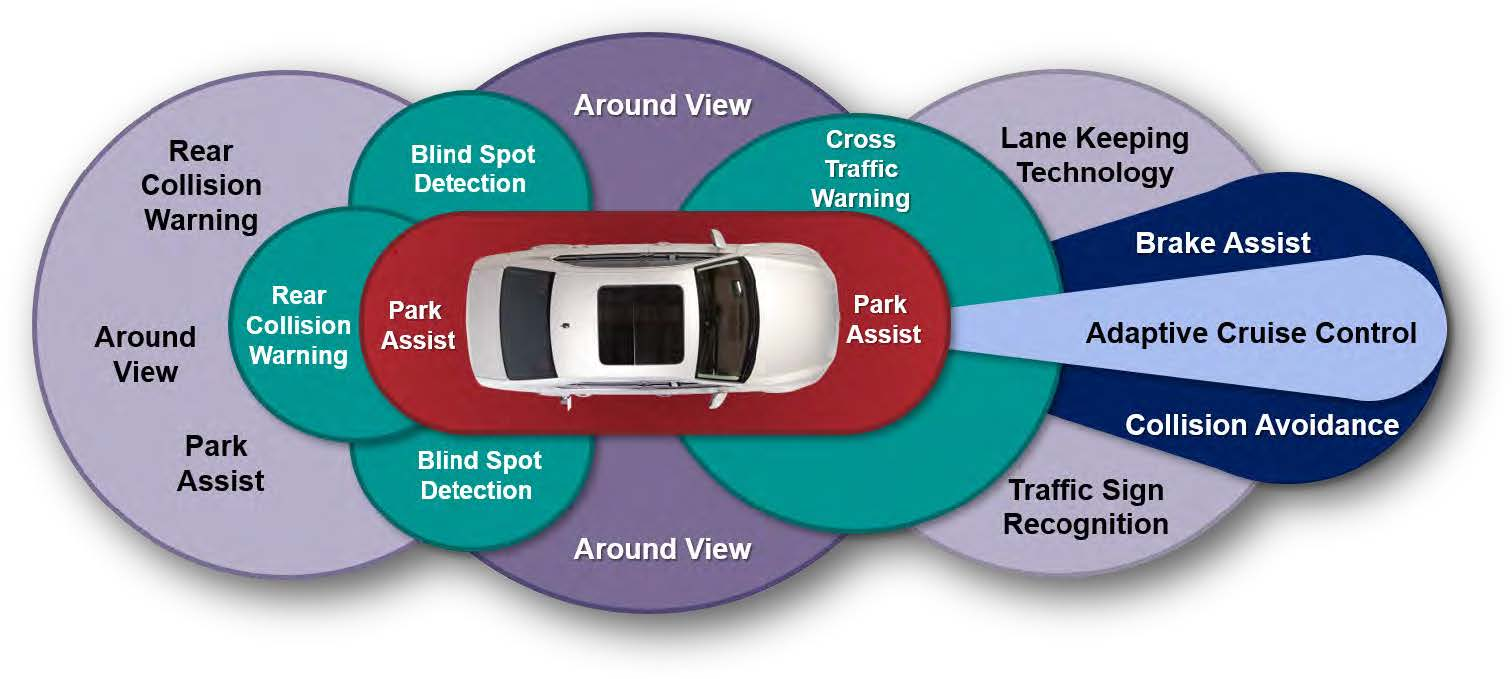
\includegraphics[width=0.6\textwidth]{Book/figures/1_introduccion/ADAS_tech.png}
    \caption{Sistema avanzado de asistencia a la conducción.}
    \label{fig:Sistema avanzado de asistencia a la conducción.}
\end{figure}

Los vehículos completamente autónomos son sistemas extremadamente complejos, por lo que actualmente no se dispone de ninguno enteramente autónomo. Por ello, mientras se avanza en el desarrollo e investigación de sistemas \ac{ADS}, son los sistemas de ayuda a la conducción o \ac{ADAS}, aquellos con los que nos podemos encontrar hoy en día. En este tipo de tecnologías es donde se centra la regulación vigente, ya que son tecnologías más probadas y que forman parte de los sistemas completamente autónomos a los que se quiere llegar. El caso de la Unión Europea muestra la evolución de la industria automovilística hacia la automatización de los sistemas de conducción, ya que a partir de julio de 2022 será obligatorio por ley el uso de tecnologías como: los sistemas de centrado en el carril, el frenado automático en caso de colisión o el uso de un sistema \ac{ISA} para regular la velocidad de los vehículos a la indicada en las vías. Todo ello para permitir obtener un mayor grado de seguridad al volante al añadir mejoras tales como las que se observan en la Figura \ref{fig:Sistema avanzado de asistencia a la conducción.}, que repercuten directamente sobre los usuarios de los vehículos \cite{adas_spain, adas_eu}.

Debido al desarrollo paulatino de estos sistemas de conducción autónoma, la \ac{SAE} ha definido 6 niveles de automatización que van del 0 (totalmente manual) al 5 (totalmente autónomo) \cite{autonomy_levels}. Estos niveles han sido adoptados por el Departamento de Transporte de los Estados Unidos, por lo que siendo un estándar actual para la clasificación de vehículos inteligentes se procede a presentar cada uno de estos niveles:

\begin{itemize}
    \item Nivel 0: La mayoría de vehículos que encontramos hoy en día en las carreteras pertenecen a este grupo, ya que con aquellos vehículos controlados manualmente.
    \item Nivel 1: Este es el nivel más bajo de automatización, ya que el vehículo cuenta únicamente con un único sistema automatizado como la dirección o la aceleración.
    \item Nivel 2: El vehículo es capaz de controlar tanto la dirección como la aceleración, pero no es un sistema autónomo ya que el conductor puede tomar el control del vehículo en cualquier momento. En esta categoría se incluyen la mayoría de los nuevos vehículos inteligentes en el mercado debido a la legislación vigente.
    \item Nivel 3: Esta clasificación se obtiene tras un gran salto tecnológico, pero para el conductor es un cambio muy sutil ya que el vehículo comienza a tener capacidades de detección del entorno lo cual permite por ejemplo, la aceleración automática del vehículo para el adelantamiento de un vehículo lento.
    \item Nivel 4: Estos vehículos son totalmente autónomos en la gran mayoría de casos, pero un conductor humano podría intervenir en una situación de emergencia. Además este tipo de vehículos suelen estar limitados en zonas urbanas a bajas velocidades.
    \item Nivel 5: Los vehículos de nivel 5 no requieren de atención humana, por lo que no será necesaria la incorporación de volante o pedales debido a su completa automatización.
\end{itemize}

\begin{figure}[H]
\centering
    \begin{subfigure}{0.45\textwidth}
    \centering
    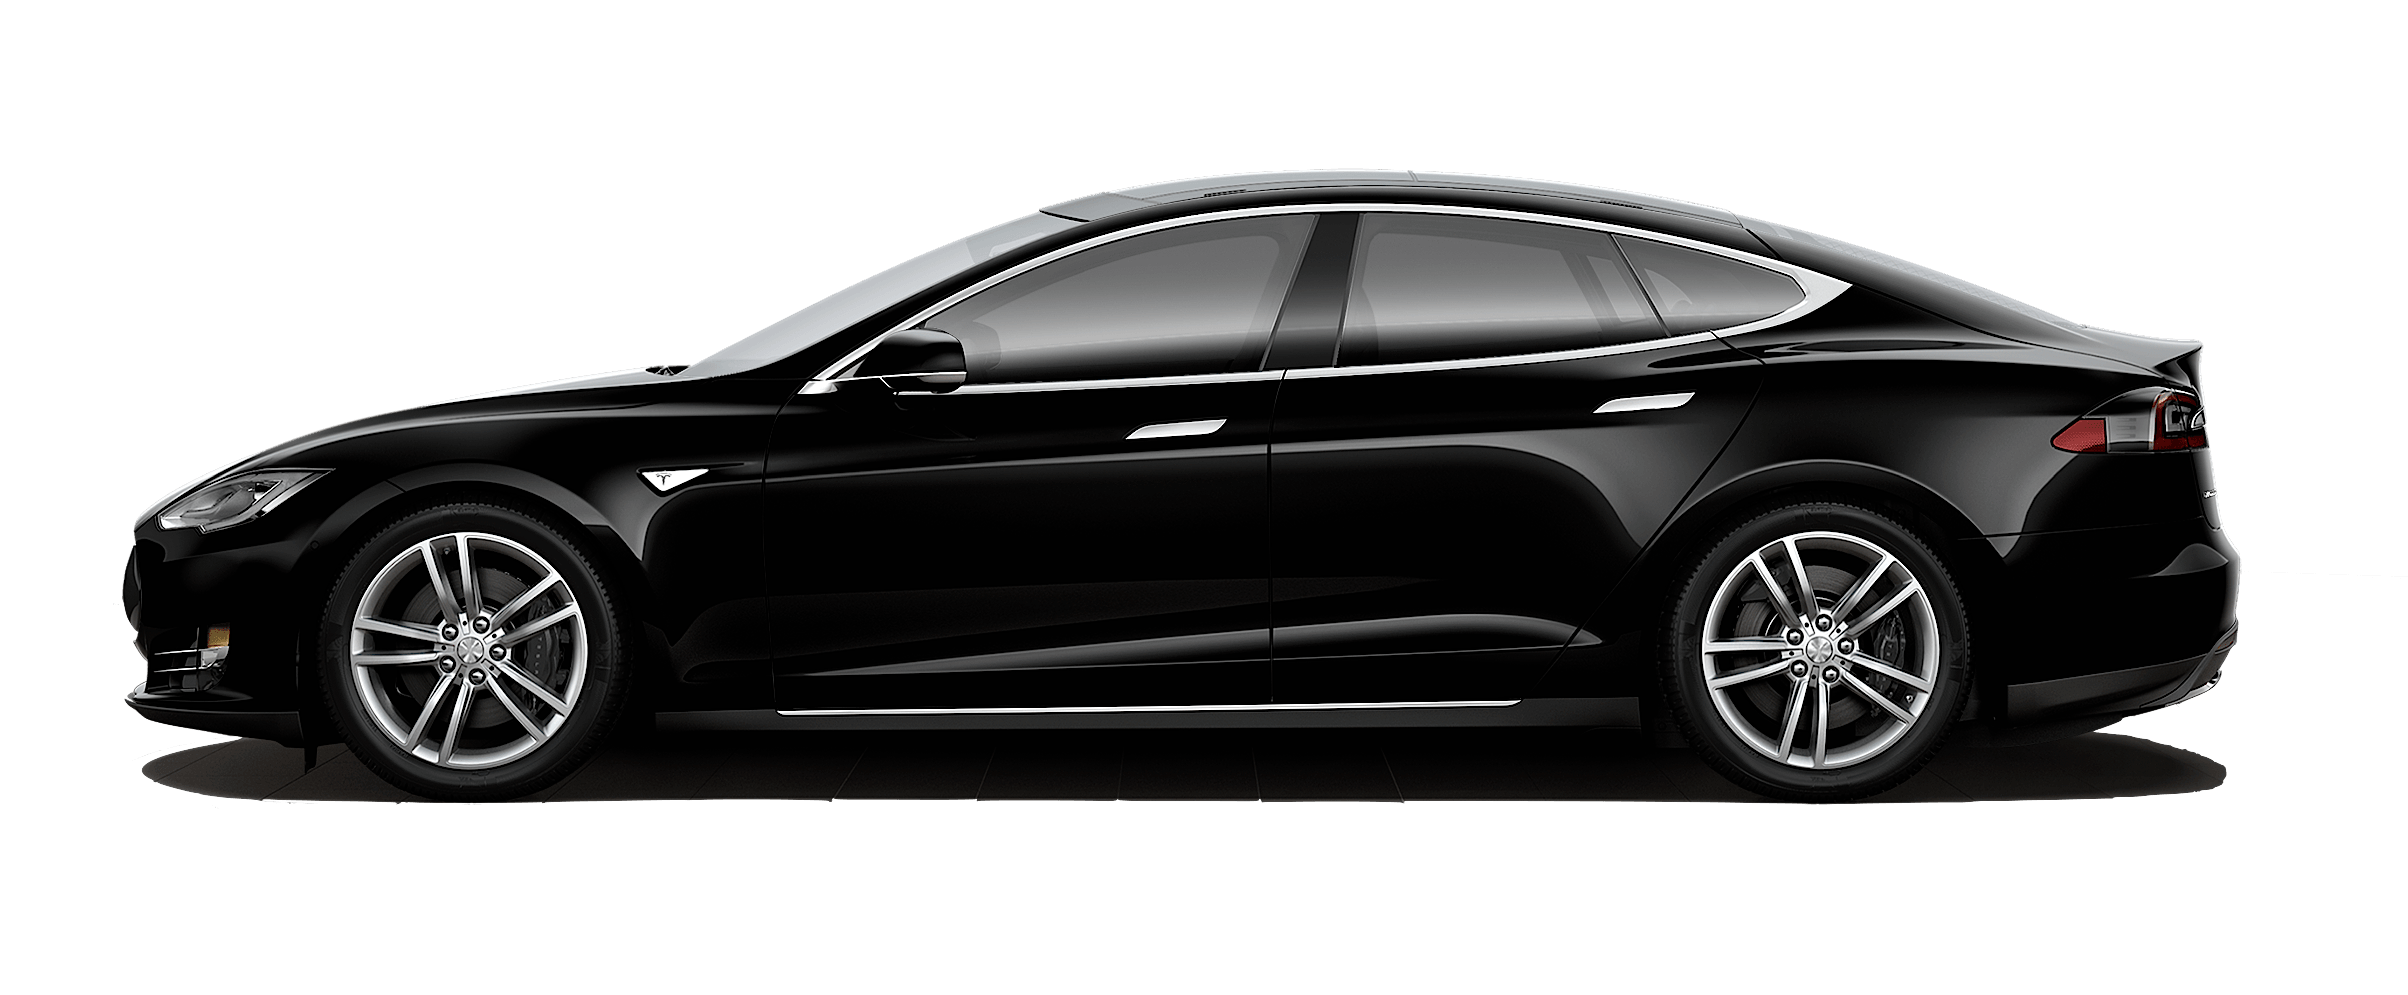
\includegraphics[width=0.95\textwidth]{Book/figures/1_introduccion/tesla.png} 
    \caption{Vehículo de Tesla.}
    \label{fig:Vehículo de Tesla.}
    \end{subfigure}
    \begin{subfigure}{0.45\textwidth}
    \centering
    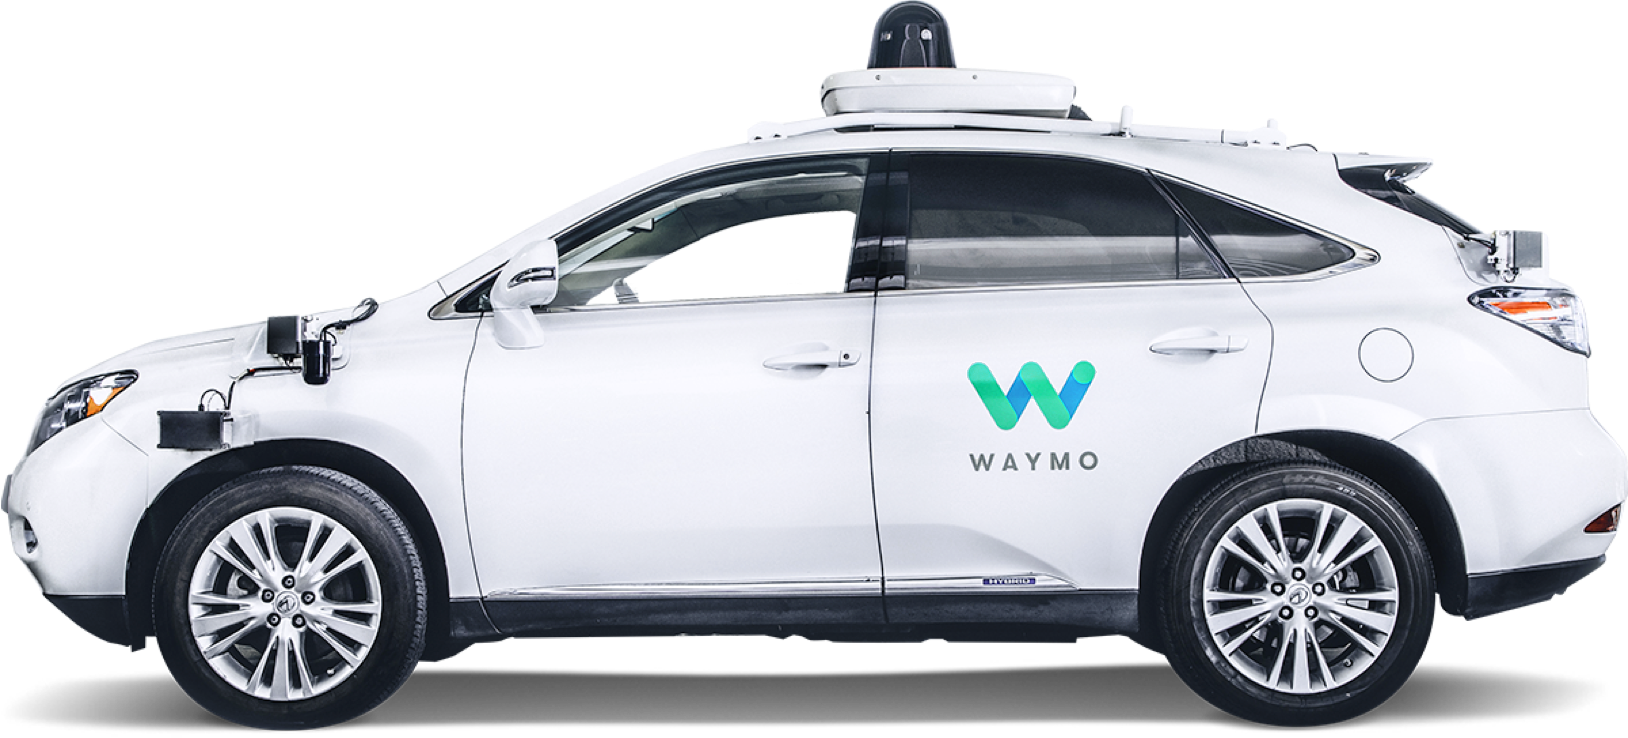
\includegraphics[width=0.85\textwidth]{Book/figures/1_introduccion/waymo.png}
    \caption{Vehículo de Waymo.}
    \label{fig:Vehículo de Waymo.}
    \end{subfigure}
\caption{Vehículos autónomos más avanzados comercializados actualmente.}
\label{fig:Vehículos autónomos más avanzados comercializados actualmente}
\end{figure}

Mientras que muchas empresas se encuentran realizando millonarias inversiones en el campo de la conducción autónoma para conseguir vehículos con la clasificación de nivel 5, entre todas ellas destaca sobre el publico general la compañía norteamericana Tesla. Pero esta no es la única empresa que está ganando mucha fama en este campo, sino que la compañía Waymo, antiguo proyecto de vehículo autónoma de Google, se encuentra entre los proyectos de creación de un vehículo de conducción autónoma completa más avanzados. Mientras que Tesla lleva años anunciando su sistema de conducción autónoma, no es hasta principios de 2022 cuando Tesla ha comenzado a mostrar la versión beta de su sistema de conducción autónoma de nivel 4. Por otra parte, Waymo se centra actualmente en la creación de una flota de taxis autónomos, este sistema se encuentra de manera funcional en Estados Unidos, en las ciudades de Phoenix y San Francisco \cite{tesla_waymo}.

Los vehículos autónomos de estas empresas no solo se diferencian en el uso actual para el cual se están comercializando, sino que como se puede observar en la Figura \ref{fig:Vehículos autónomos más avanzados comercializados actualmente}, ambos vehículos utilizan diferentes sensores para observar el entorno que les rodea. Mientras que Tesla opta por una aproximación más barata utilizando cámara y \ac{Radar}, Waymo añade al menos en la parte superior de sus vehículos un \ac{LiDAR} para la conseguir un sistema más robusto, aunque menos económico. Por lo que el desarrollo de este tipo de tecnologías puede optar por múltiples aproximaciones o configuraciones pero teniendo siempre en mente la consecución de un sistema completamente autónomo de nivel 5.

\section{Sistemas de detección de objetos}
\label{sec:Sistemas de detección de objetos}

Una de las principales tareas que realizan los vehículos autónomos es la detección de objetos, el cual se suele realizar de forma previa al seguimiento de objetos, la estimación de la trayectoria y la evitación de colisiones. Los objetos a atender en la carretera, como son: peatones, ciclistas, coches; lo cual supone un reto mayor para la creación de sistemas fiables y robustos para la detección de objetos. La mayoría de los vehículos autónomos disponibles en el mercado, así como la investigación sobre ellos, dependen del empleo de sensores costosos \cite{paper_object_detection}.

\begin{figure}[H]
    \centering
    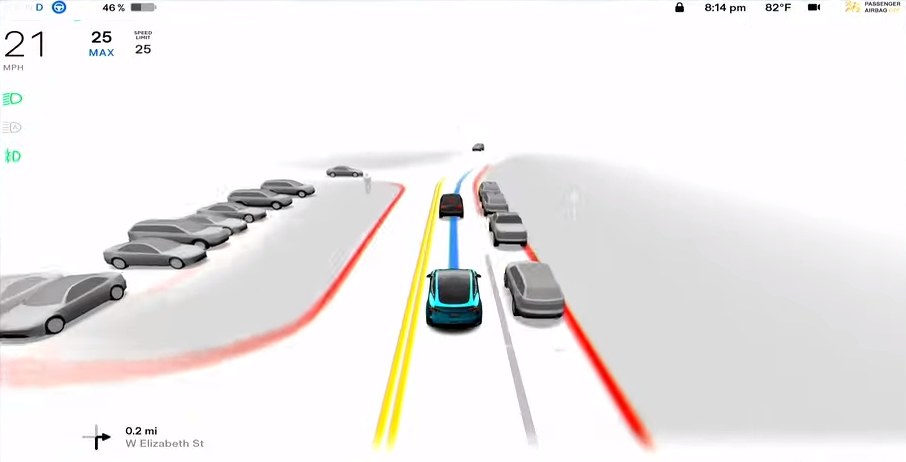
\includegraphics[width=0.65\textwidth]{Book/figures/1_introduccion/HMI_Tesla.png}
    \caption{Interfaz Humano Máquina de la beta del Tesla FDS.}
    \label{fig:Interfaz Humano Máquina de la beta del Tesla FDS.}
\end{figure}

Atendiendo a los diferentes sistemas de detección con los que se puede trabajar, encontramos los sistemas de detección 2D y detección 3D. Mientras que los sistemas de detección 2D llevan a cabo una detección de los objetos del entorno sobre el plano de las imágenes dadas por las cámaras del vehículo. Los sistemas de detección 3D pueden hacer uso de diferentes sensores para mejorar la comprensión del entorno que rodea al propio vehículo al añadir una nueva dimensión que define la profundidad, la Figura \ref{fig:Interfaz Humano Máquina de la beta del Tesla FDS.} muestra la capacidad de percepción 3D en los vehículos Tesla. Los métodos de detección 3D no solo se basan en cámaras sino que también son utilizados \ac{LiDAR} y \ac{Radar} para conseguir un sistema más preciso, ya que estos sensores se pueden utilizar tanto de forma individualizada como en conjunto para obtener un sistema de detección más robusto.

Debido a la variedad de aproximaciones que se pueden tomar en cuanto al uso de sensores para obtener un sistema de detección de objetos 3D, se procede a presentar los principales sensores utilizados tanto en la industria automovilística como en este trabajo.

\subsection{Cámara}
\label{sec:Cámara}

Los sistemas basados en cámara son los más utilizados tanto en sistemas \ac{ADAS} como sistemas \ac{ADS}, ya que permiten de forma pasiva obtener imágenes de forma continua del entorno que rodea al vehículo. Los sistemas basados en cámara tienen diferentes variaciones que se pueden utilizar, entre ellas encontramos los sistemas monoculares y los estereoscópicos. Mientras que los sistemas de cámara monoculares hacen uso de una única cámara, los sistemas de cámaras estéreo utilizan dos cámaras individuales para lograr extraer la información de profundidad de la escena a partir de técnicas como la fotogrametría, obteniendo resultados como los visibles en la Figura \ref{fig:Mapa de profundidad creado a partir de un sistema estéreo.}.

\begin{figure}[H]
    \centering
    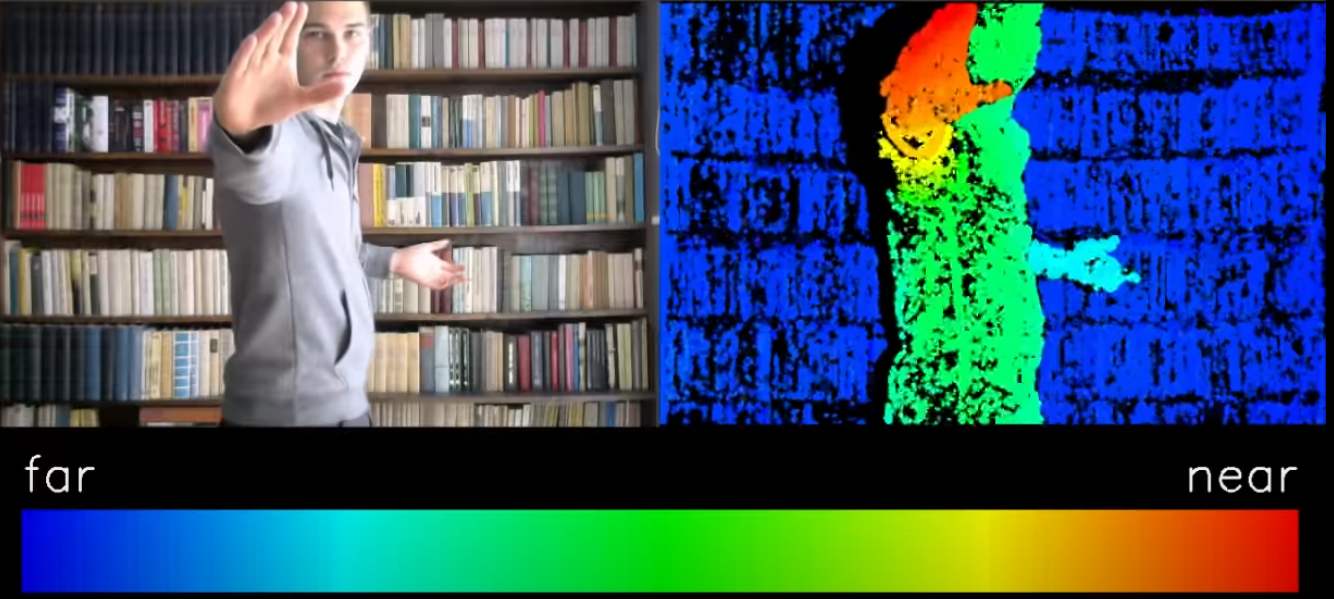
\includegraphics[width=0.65\textwidth]{Book/figures/1_introduccion/stereo_system.png}
    \caption{Mapa de profundidad creado a partir de un sistema estéreo.}
    \label{fig:Mapa de profundidad creado a partir de un sistema estéreo.}
\end{figure}

% \begin{figure}[H]
% \centering
%     \begin{subfigure}{0.45\textwidth}
%     \centering
%     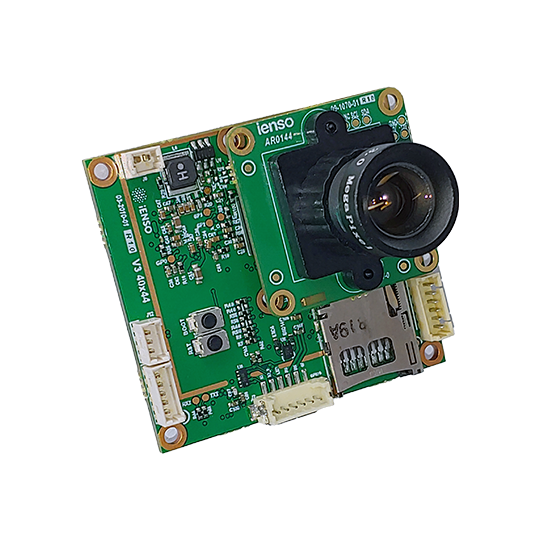
\includegraphics[width=0.5\textwidth]{Book/figures/1_introduccion/monocular_camera.png} 
%     \caption{Sistema monocular.}
%     \label{fig:Sistema monocular.}
%     \end{subfigure}
%     \begin{subfigure}{0.45\textwidth}
%     \centering
%     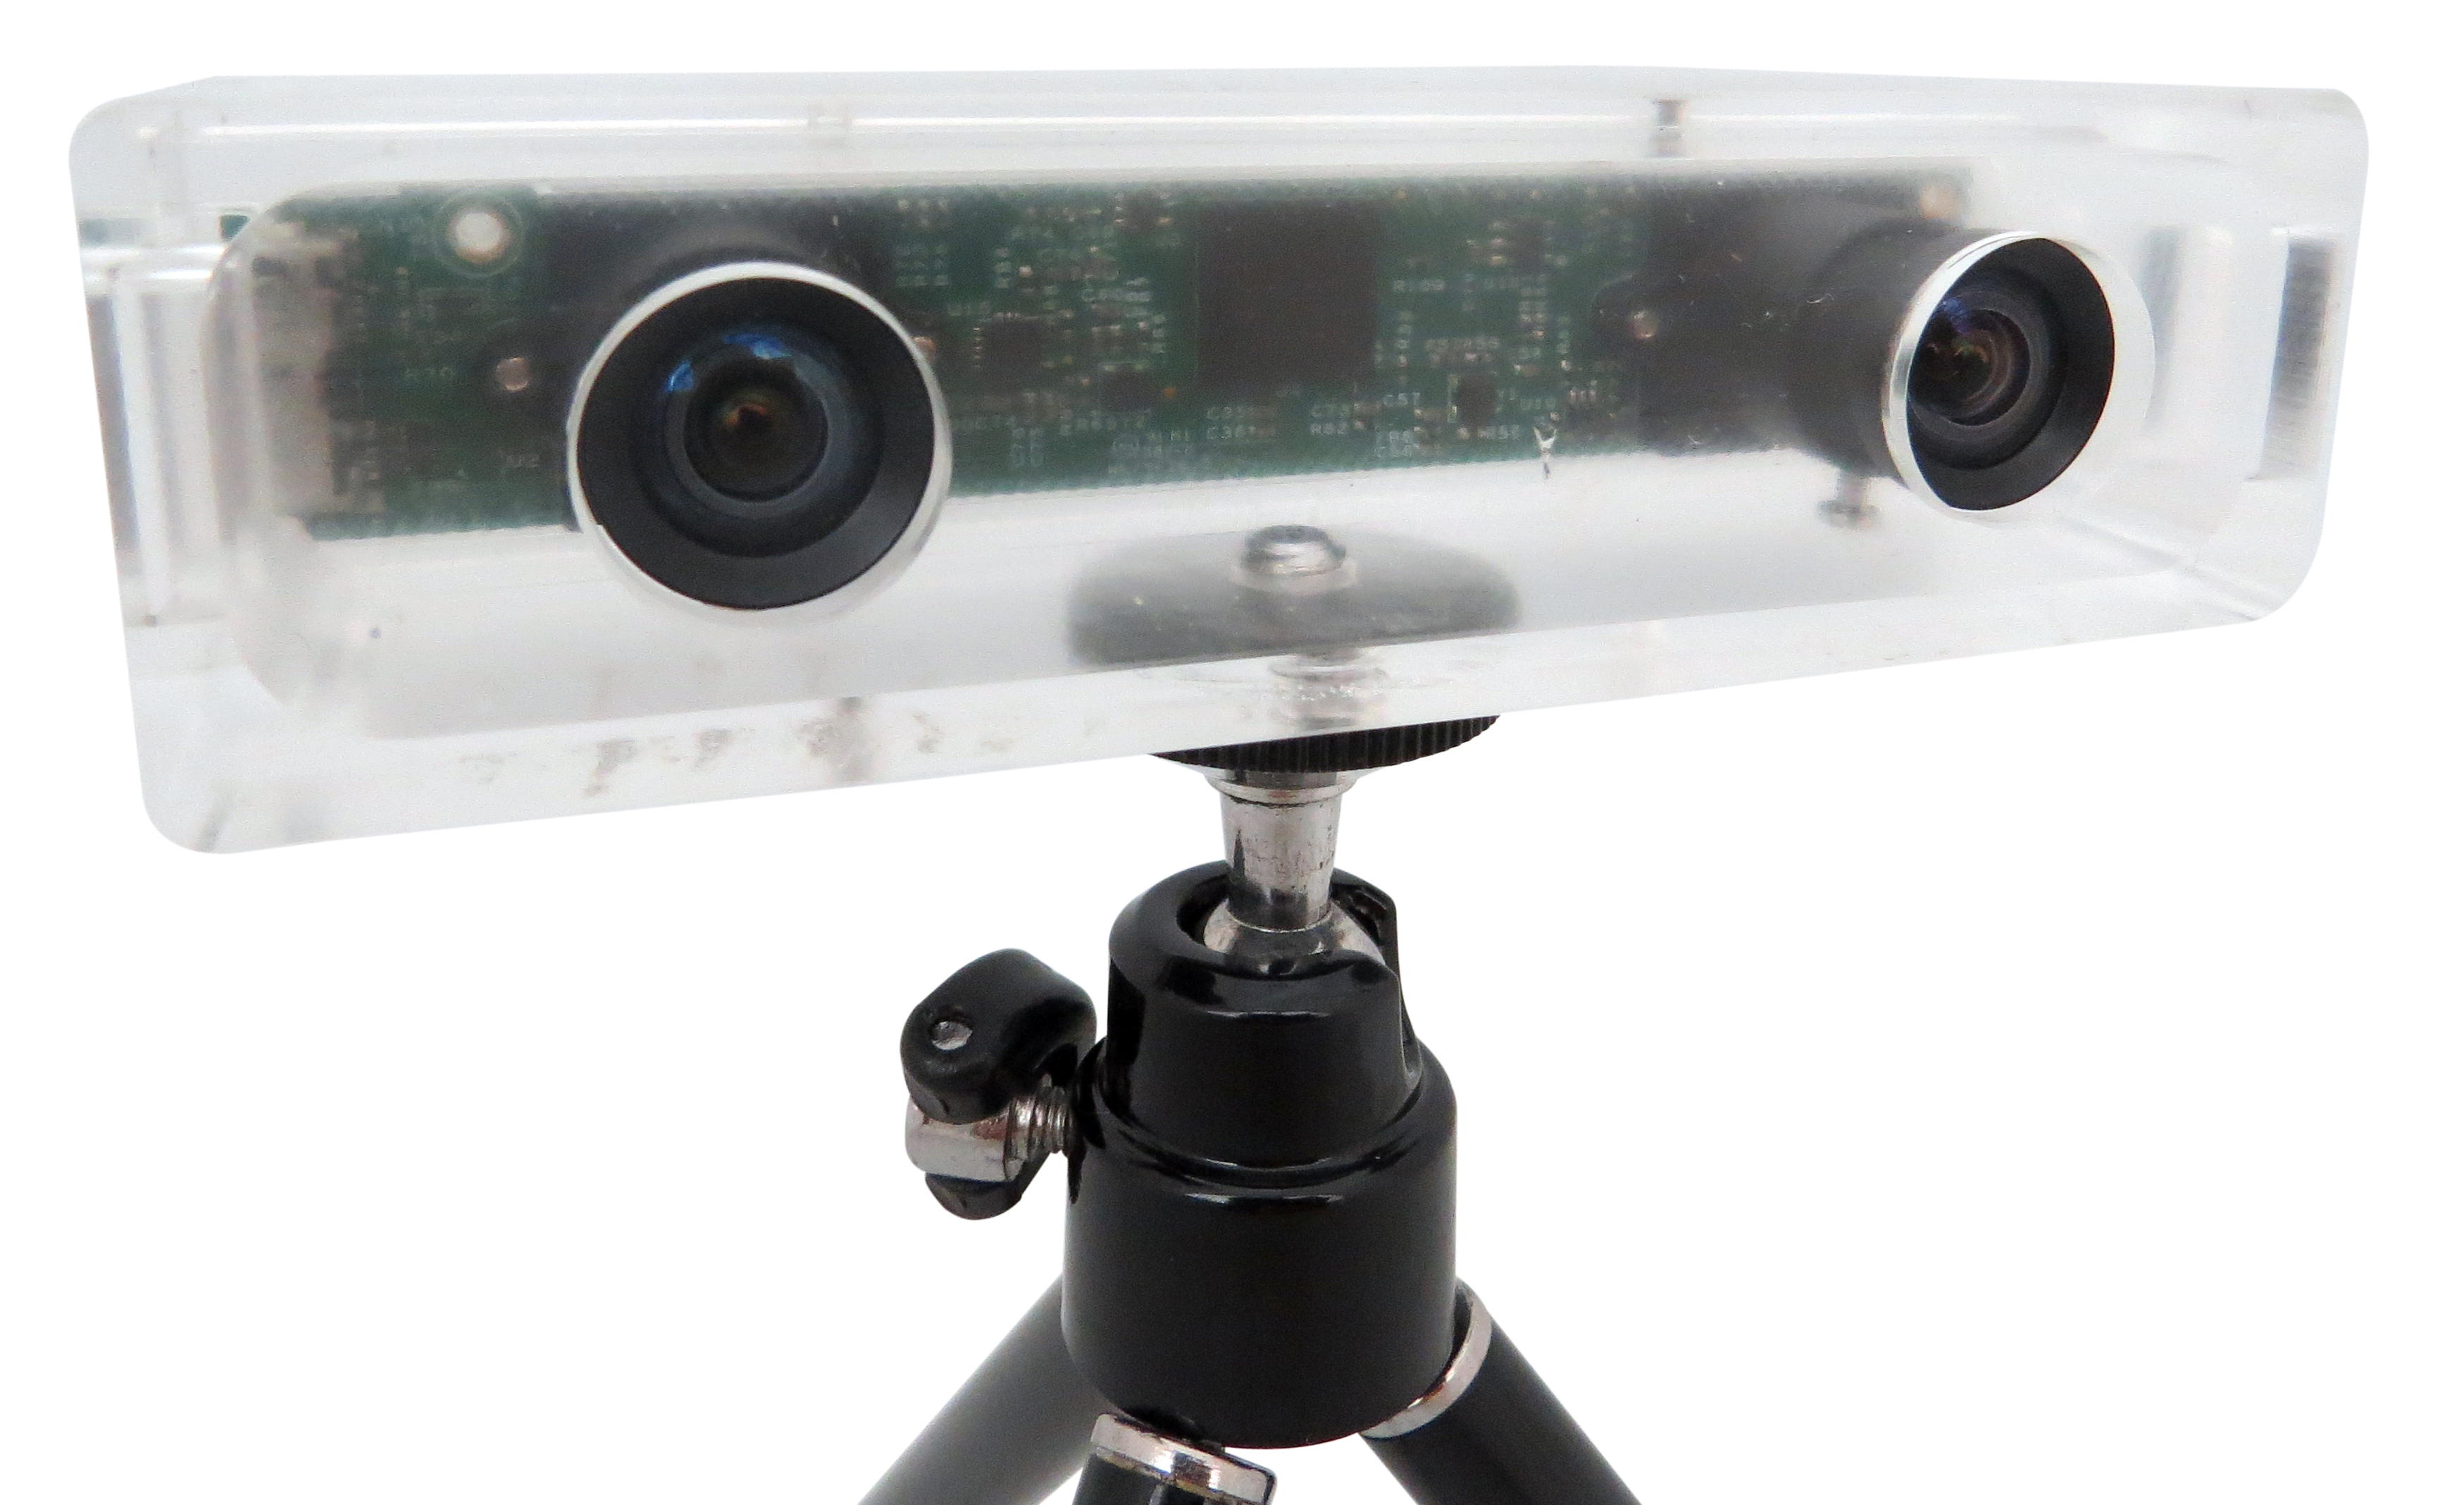
\includegraphics[width=0.85\textwidth]{Book/figures/1_introduccion/stereo_camera.png}
%     \caption{Sistema estéreo.}
%     \label{fig:Sistema estéreo.}
%     \end{subfigure}
% \caption{Diferentes sistemas de cámaras utilizados.}
% \label{fig:Diferentes sistemas de cámaras utilizados.}
% \end{figure}

Hay empresas como Tesla que basan gran parte de su sistema de conducción autónomo alrededor del uso de cámaras, debido a las ventajas que ofrece este sensor. Las cámaras son capaces de capturar la información de color, textura y contraste de forma directa, y además debido al gran estudio de técnicas basadas en Deep Learning durante los últimos años para obtener la mayor cantidad de información posible, es muy sencilla la obtención de detalles de alto nivel. Todas estas características, combinadas con gran resolución de píxeles y un bajo coste, han convertido a las cámaras en el principal candidato para los sistemas \ac{ADAS} \cite{advantages_camera}.

El uso de este sensor no se encuentra sin inconvenientes, ya que en condiciones climáticas adversas como niebla o lluvia se pierde gran parte de la información recabada por el sensor. De la misma manera que el ojo humano, las cámaras sufren con grandes cambios en la luminosidad del entorno, ya que se pueden dejar regiones sin visibilidad ninguna, como ocurre en túneles, al dirigir la cámara hacia el Sol o al conducir de noche en zonas muy oscuras. La obtención de la profundidad utilizando sistemas de cámaras requiere de un proceso muy complejo y que puede derivar en grandes errores. Por último, y como desventaja siempre presente se encuentra la necesidad de modelos basados en Deep Learning que típicamente requiere del uso de plataformas de aceleración por hardware para su uso en tiempo real \cite{paper_comparison_lidar_camera}.

\subsection{LiDAR}
\label{sec:LiDAR}

La tecnología \ac{LiDAR} se basa en la detección de los haces de luz que son emitidos por un haz de luz láser con una intensidad definida de antemano, y mide el tiempo de llegada del haz reflejado detectado por los fotodiodos que se encuentran en el sensor \cite{paper_comparison_lidar_camera, what_lidar}. Este proceso de cálculo del tiempo de llegada de cada haz láser enviado, produce una nube de puntos la cual genera un punto $(x, y, z, i)$, por cada uno de los haces de luz enviados, ya que conociendo la velocidad de la luz, el tiempo de retorno de cada haz y el ángulo de inclinación desde el que se envió, se obtiene la posición tridimensional, además del coeficiente de reflexión del objeto sobre el que el ha incidido cada rayo.

No todos los \ac{LiDAR} son iguales, ya que encontramos tanto sensores fijos que producen una nube de puntos de la parte frontal al sensor, como los encontrados en los nuevos iPhone Pro; sensores que producen una nube de puntos bidimensional al tener una plataforma giratoria con un único láser, como los utilizados en robótica móvil; y sensores con múltiples láser posicionados de forma vertical de modo que el girar mediante una plataforma giratoria producen una nube de puntos 3D, este tipo de \ac{LiDAR} es el que principalmente se utiliza para el diseño de vehículos autónomo, un ejemplo de la salida de este tipo sensores es la nube de puntos que se muestra en la Figura \ref{fig:Nube de puntos producida por un LiDAR 3D.}.

\begin{figure}[H]
    \centering
    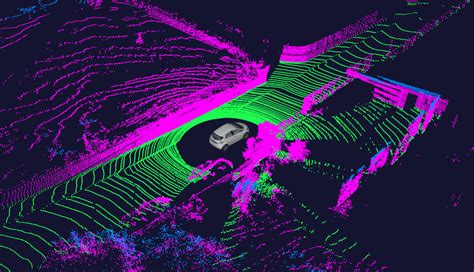
\includegraphics[width=0.6\textwidth]{Book/figures/1_introduccion/pointcloud.png}
    \caption{Nube de puntos producida por un LiDAR 3D.}
    \label{fig:Nube de puntos producida por un LiDAR 3D.}
\end{figure}

Entre las ventajas que se obtienen al utilizar un sensor \ac{LiDAR} en relación a una cámara encontramos: la precisión en las medidas tomadas, ya que el propio sensor tiene un grado de error muy reducido; el uso de los datos del \acs{LiDAR} para la obtención de la profundidad no requiere de un procesamiento previo, por lo que se puede utilizar este dato directamente recibido del sensor; las condiciones lumínicas y meteorológicas adversas no repercuten en la posibilidad de uso de dicho sensor, ya que aunque se disminuye la calidad de los datos en situaciones muy adversas, es completamente utilizable.

Al contrario, se encuentran ciertas desventajas en su uso, como la dificultad de interpretabilidad de este sensor, las condiciones climáticas en las que la obtención de datos no es perfecta y el más influyente de todos, el alto precio de este sensor que puede ascender a 100.000 dolares por un único sensor. Debido al factor monetario, este sensor no es utilizado en los vehículos de la marca Tesla ya que aumentaría considerablemente el precio de sus vehículos, aunque la gran mayoría de empresas que tratan de construir un sistema autónomo apuestan por este sensor como parte de su sistema de percepción.

\subsection{Fusión sensorial}
\label{sec:Fusión sensorial}

El uso de sensores individuales puede proporcionar información útiles del entorno que se quiere comprender. Por esto mismo, la combinación de sensores para la obtención de un sistema de percepción más preciso es un proceso que nos permite generar modelos de percepción más robustos y con menos fallos. Esto nos permite diseñar un modelo mucho mejor del mundo que nos rodea, suponiendo que el todo es mayor que la suma de sus partes. La fusión de sensores es el proceso mediante el cual podemos lograr unificar las bondades de los sensores utilizados tratando de minimizar las desventajas de cada uno de ellos \cite{what_fusion}.

Al realizar un proceso de fusión sensorial se presentan múltiples aproximaciones sobre las cuales se puede trabajar: si se realizar una unión de la información de las diferentes fuentes o en este caso sensores para construir un modelo que tome como entrada ese conjunto de datos, se trata de una 'early fusion', en cambio, si se realiza un procesamiento por cada una de las fuentes de datos y se terminan uniendo las salidas de los diferentes modelos, se obtiene un modelo basado en una 'late fusion'. Estas no son las únicas opciones disponibles, ya que entre ambas técnicas se encuentran los modelos basados en 'middle fusion' estos modelos utilizan las fuentes de datos parcialmente procesadas para unirlas y posteriormente completar el pipeline de dicho modelo, como se ve en la Figura \ref{fig:Flujo de trabajo basado en fusión sensorial.}.

\begin{figure}[H]
    \centering
    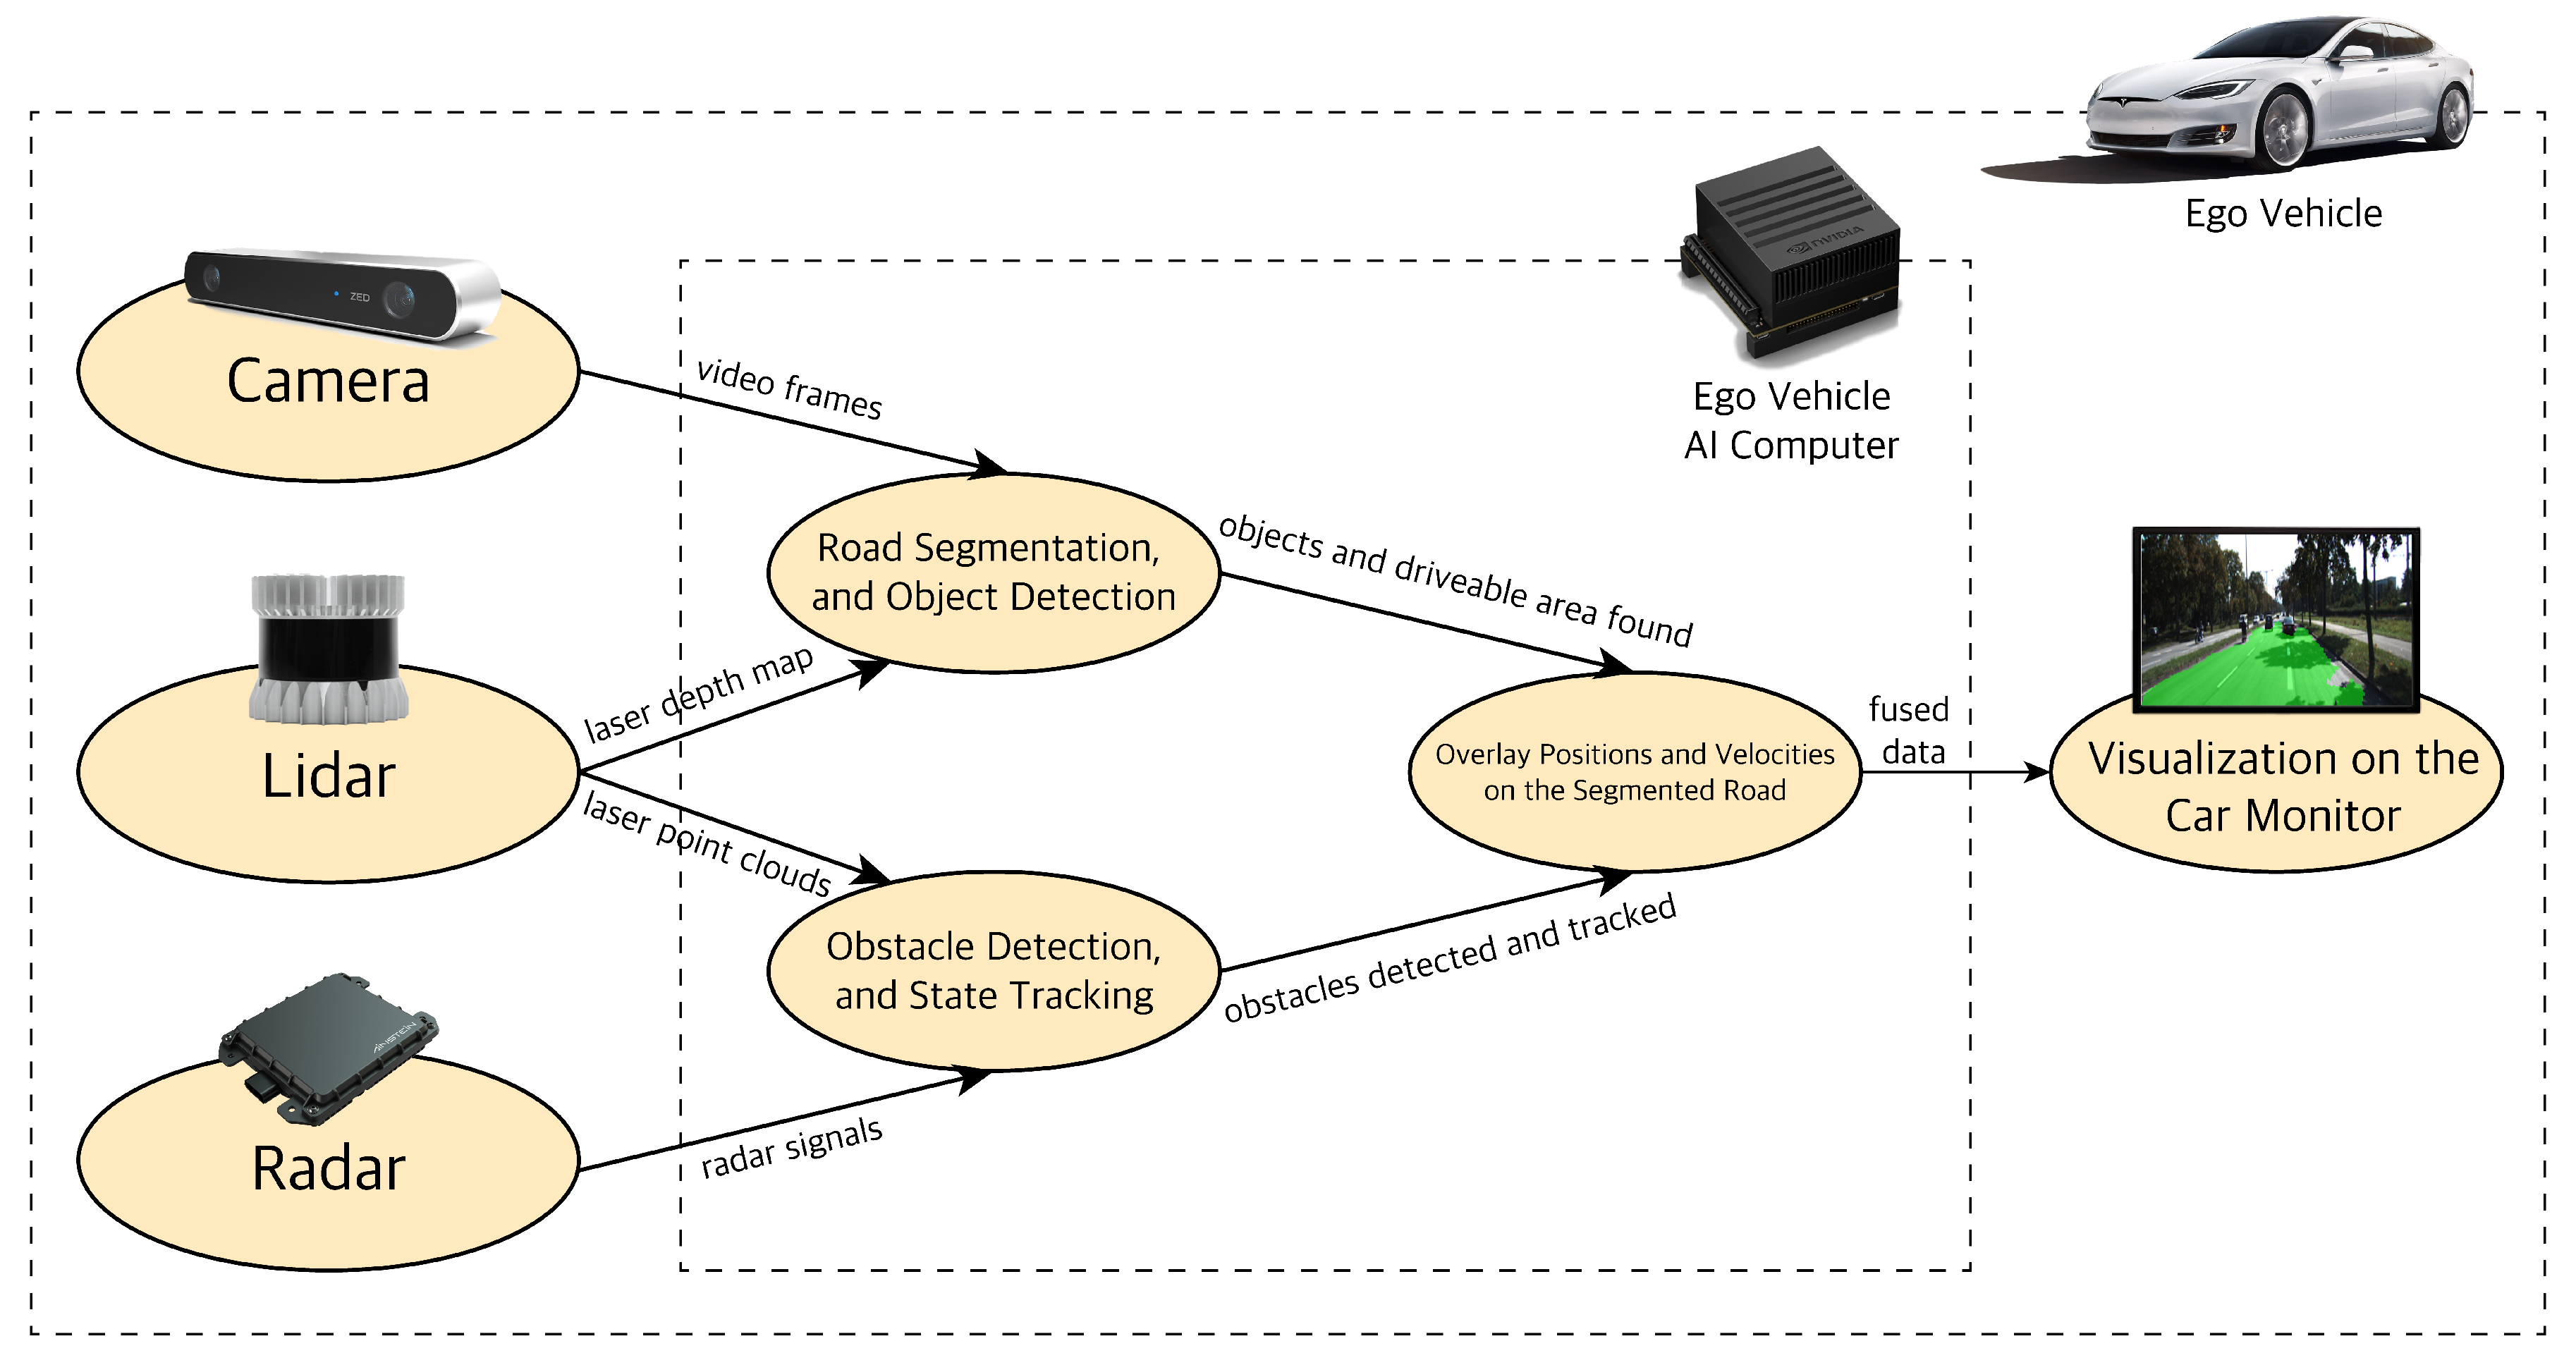
\includegraphics[width=0.7\textwidth]{Book/figures/1_introduccion/ejemplo_fusion.png}
    \caption{Flujo de trabajo basado en fusión sensorial.}
    \label{fig:Flujo de trabajo basado en fusión sensorial.}
\end{figure}

La creación de modelos de percepción basados en fusión sensorial aporta grandes ventajas sobre el uso de un único sensor, ya que permite generar sistemas más precisos y robustos al tratar de reducir las desventajas individuales de cada sensor. Entre las desventajas del uso de estos sistemas se encuentra, la complejidad en la creación del sistema completo de percepción al utilizar diferentes sensores y tecnologías, pero sobre todo el elevado coste que supone la adquisición de múltiples sensores por cada sistema de percepción. Siendo típicamente el coste, el factor vital para la producción a gran escala, la gran mayoría de las empresas basadas en la creación de sistemas de conducción autónomos abogan por el uso de esta tecnología, principalmente utilizando cámara, \ac{LiDAR} y \ac{Radar} entre otros sensores.

\section{Machine Learning}
\label{sec:Machine Learning}

El aprendizaje automático o \ac{ML} es una rama de la inteligencia artificial y la computación que se centra en el uso de datos y algoritmos para mejorar gradualmente su precisión. Mediante el uso de métodos estadísticos, los algoritmos se entrenan para hacer clasificaciones o predicciones, descubriendo ideas clave dentro de proyectos aplicando técnicas de minería de datos \cite{what_ml}.

Dentro de este amplio campo de conocimiento encontramos principalmente 4 grupos de técnicas para creación de modelos de aprendizaje automático \cite{ml_techs}:

\begin{itemize}
    \item Aprendizaje supervisado: En el caso de conocer de antemano que es lo que quiere enseñar a la máquina y se parte de una gran cantidad de datos anotados, se puede conseguir generar un modelo que se ajuste para que minimice el error al realizar la tarea que se le ha encomendado.
    \item Aprendizaje no supervisado: Este conjunto de técnicas trata de descubrir patrones ocultos que relacionen diversas variables. Además no suele requerir de grandes cantidades de datos de entrada por lo que el proceso de entrenamiento es reducido.
    \item Aprendizaje semisupervisado: Los modelos semisupervisados tratan de hacer el máximo uso de unos pocos datos etiquetados y gran cantidad de datos no etiquetados para realizar una tarea concreta.
    \item Aprendizaje por refuerzo: Mediante la interacción de una máquina con un entorno en el que poder realizar determinadas acciones que pueden ser recompensadas o castigadas, es posible generar un modelo que realice la tarea que debía realizar sin presentar explícitamente el cómo.
\end{itemize}

\begin{figure}[H]
    \centering
    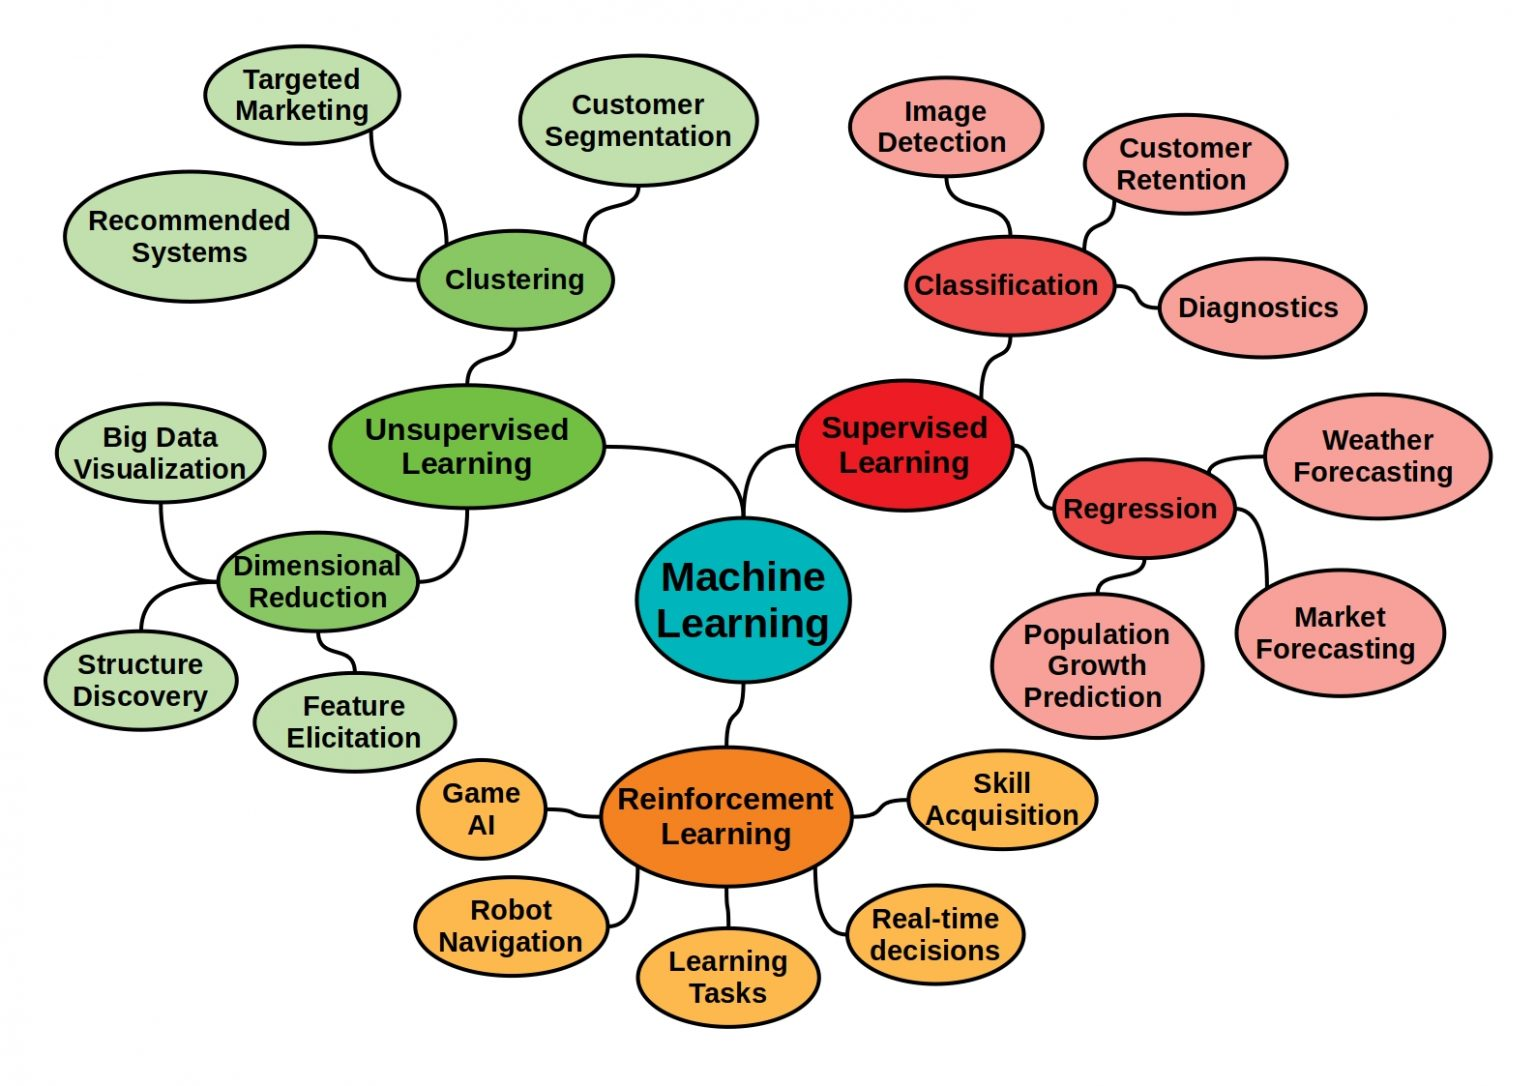
\includegraphics[width=0.6\textwidth]{Book/figures/1_introduccion/ml_techniques.png}
    \caption{Principales campos de estudio de estudio del Machine Learning.}
    \label{fig:Principales campos de estudio de estudio del Machine Learning.}
\end{figure}

A partir de estos grupos de técnicas se encuentran gran cantidad de subgrupos, como se observa en la Figura \ref{fig:Principales campos de estudio de estudio del Machine Learning.} y de técnicas concretas, pero entre todas estás técnicas, aquella que está revolucionando múltiples campos de estudio y que está propiciando grandes avances es el Deep Learning.

\subsection{Deep Learning}
\label{sec:Deep Learning}

El Deep Learning o aprendizaje profundo, es un subconjunto del campo del aprendizaje automático que consiste en el uso de redes neuronales con más una capa oculta. Dichas redes neuronales se inspiran en el cerebro humano imitando la forma en las que las neuronas biológicas se comunican entre sí. Estas se componen de una capa de nodos de entrada, una o más capas de ocultas y una capa de salida, en la que cada nodo se conecta otro y tiene un peso y umbral asociados. Si la salida de cualquier nodo individual está por encima del valor umbral especificado, ese nodo se activa, enviando datos a la siguiente capa de la red. En caso contrario, no se transmite ningún dato a la siguiente capa de la red \cite{what_nn}.

La Figura \ref{fig:Modelo básico de Deep Learning.} muestra por tanto un modelo basado en Deep Laerning ya que incorpora al menos dos capas intermedias. Mientras que una red neuronal con una sola capa puede hacer predicciones aproximadas, las capas adicionales pueden ayudar a optimizar y refinar la precisión. Los modelos basados en Deep Learning son utilizados en multitud de aplicaciones y servicios del día a día y realizan tareas analíticas y físicas sin intervención humana \cite{what_dl}. 

\begin{figure}[H]
    \centering
    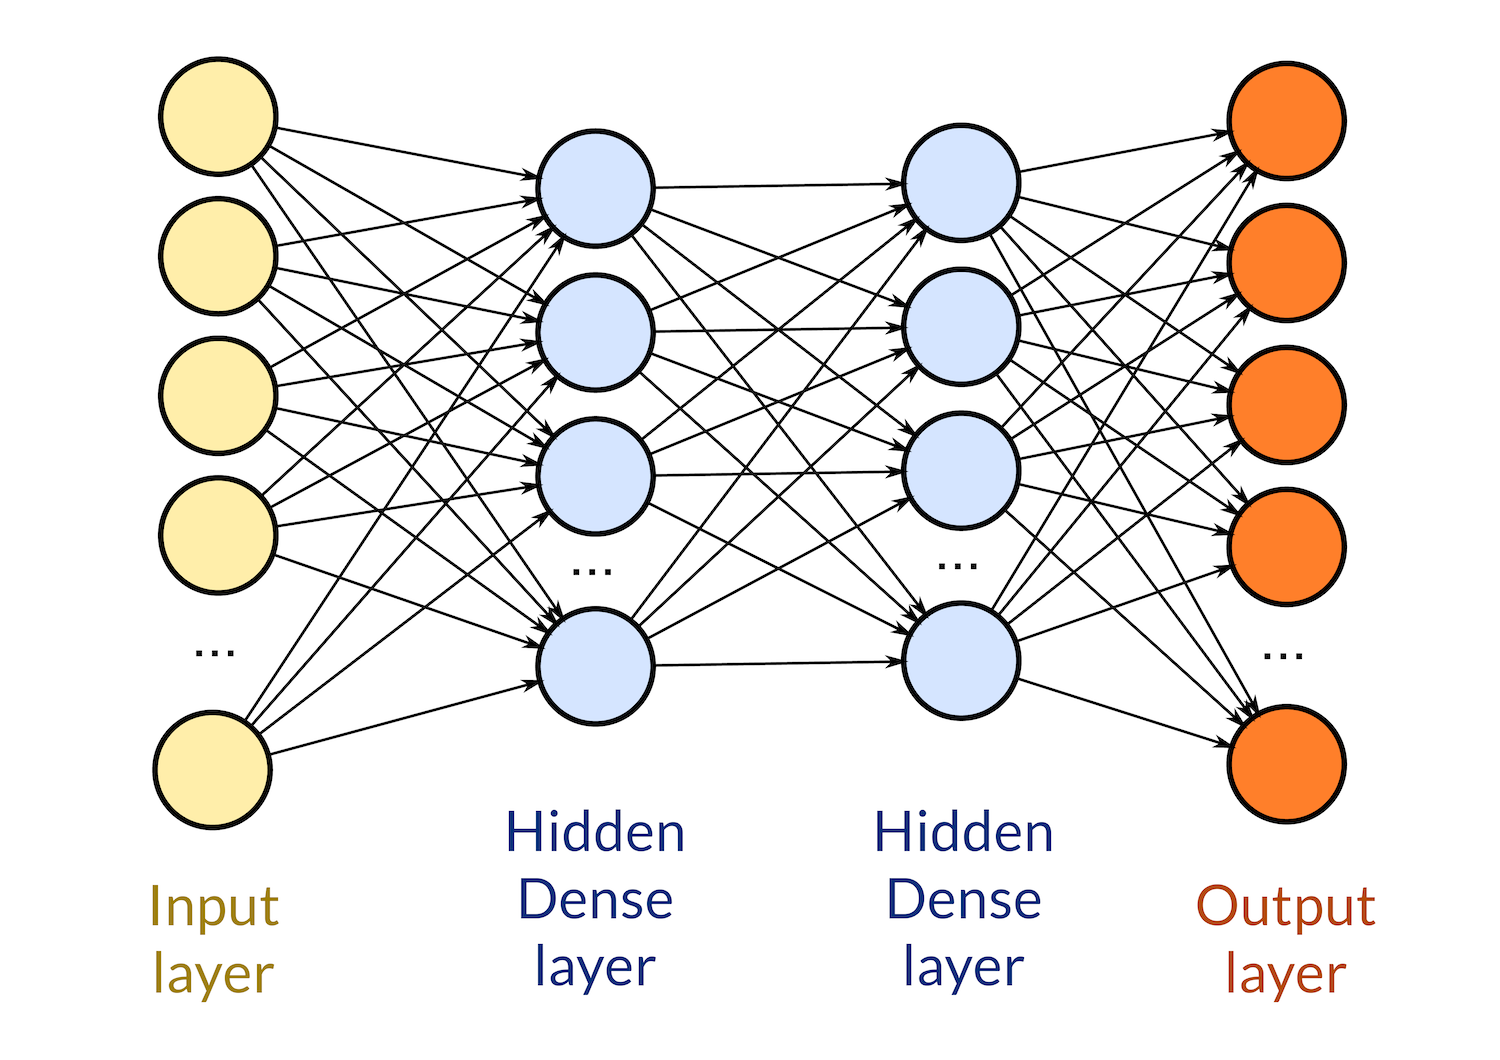
\includegraphics[width=0.6\textwidth]{Book/figures/1_introduccion/dl_model.png}
    \caption{Modelo básico de Deep Learning.}
    \label{fig:Modelo básico de Deep Learning.}
\end{figure}

Muchos campos de estudio han mejorado gracias a esta tecnología y otros están sufriendo un cambio tan radical que abren a puerta a multitud de nuevas aplicaciones que pueden ser muy beneficiosas. Entre los campos afectados por el Deep Learning encontramos:

\begin{itemize}
    \item Visión por computador: Durante los últimos años, los modelos basados en \ac{CNN} (explicados en el Capítulo \ref{sec:Convolutional Neural Networks}) han permitido el uso de sistemas de visión por computador en entornos menos controlados, ya que proporcionan una mejora espectacular en precisión en comparación con los algoritmos tradicionales de procesamiento de imágenes.
    \item Procesamiento del lenguaje natural: Tras su salida en 2020, GPT-3 \cite{GTP3} ha presentado un gran avance en el mundo del \ac{NLP} ya que ha conseguido un rendimiento inigualable hasta la fecha con grandes mejoras que vislumbran un futuro con inteligencias artificiales de carácter general.
    \item Creación de medicamentos: Dentro del campo de la medicina, hay una rama de métodos que tratan de predecir que estructura de las proteínas son las más eficaces en combatir una enfermedad. La empresa DeepMind tras la presentación del modelo basado en Deep Learning, AlphaFold \cite{AlphaFold}, y conseguir superar con amplias creces la competición \ac{CASP} que se basa en la predicción de la estructura de las proteínas, ha conseguido situarse a la cabeza de este campo democratizando a su vez el acceso a desarrollar de nuevas tecnologías a partir de esta.
\end{itemize}

Como se ha presentado, el Deep Learning engloba un conjunto de técnicas ampliamente utilizadas, esto es debido principalmente a que permite maximizar el uso de datos no estructurados, obtiene en gran cantidad de los casos unos muy buenos resultados y no requiere de una perfecta aplicación de 'feature engineering'. Como contraparte a su uso encontramos: la gran cantidad de datos que se necesitan para la creación de un modelo, la necesidad de un conocimiento especializado en las técnicas Deep Learning aplicadas al campo en el que se trabaja, y la necesidad de una gran potencia computacional para el entrenamiento de los modelos \cite{adv_disafv_dl}.

\chapter{Estado del arte en técnicas de fusión sensorial}
\label{cha:Estado del arte en técnicas de fusión sensorial}

\begin{FraseCelebre}
  \begin{Frase}
    Texto.
  \end{Frase}
  \begin{Fuente}
    Autor texto
  \end{Fuente}
\end{FraseCelebre}

\section{MV3D}
\label{sec:MV3D}

\section{Frustum PointNets}
\label{sec:Frustum PointNets}

\section{PointPainting}
\label{sec:PointPainting}

\chapter{Propuesta de trabajo}
\label{cha:Propuesta de trabajo}

\begin{FraseCelebre}
  \begin{Frase}
    Texto.
  \end{Frase}
  \begin{Fuente}
    Autor texto
  \end{Fuente}
\end{FraseCelebre}

% https://arxiv.org/abs/1812.04244 (PointRCNN 2 stages)
\chapter{KITTI Dataset}
\label{cha:KITTI Dataset}

\begin{FraseCelebre}
  \begin{Frase}
    Texto.
  \end{Frase}
  \begin{Fuente}
    Autor texto
  \end{Fuente}
\end{FraseCelebre}

\section{Contenido del dataset}
\label{sec:Contenido del dataset}

\section{Sistema de evaluación}
\label{sec:Sistema de evaluación}

\chapter{Sistema de detección 2D con cámara}
\label{cha:Sistema de detección 2D con cámara}

\begin{FraseCelebre}
  \begin{Frase}
    Texto.
  \end{Frase}
  \begin{Fuente}
    Autor texto
  \end{Fuente}
\end{FraseCelebre}

\section{Técnicas de Deep Learning aplicadas a detección 2D}
\label{sec:Técnicas de Deep Learning aplicadas a detección 2D}

\subsection{Convolutional Neural Networks}
\label{sec:Convolutional Neural Networks}

\subsection{Transfer learning}
\label{sec:Transfer learning}

\section{YOLOv5}
\label{sec:YOLOv5}

\section{Entrenamiento y evaluación de YOLOv5}
\label{sec:Entrenamiento y evaluación de YOLOv5}

\chapter{Sistema de aproximación de la distancia}
\label{cha:Sistema de aproximación de la distancia}

\begin{FraseCelebre}
  \begin{Frase}
    Texto.
  \end{Frase}
  \begin{Fuente}
    Autor texto
  \end{Fuente}
\end{FraseCelebre}

\noindent
Obteniendo las detecciones 2D de los objetos dentro del \ac{FoV} de la cámara utilizada, se procede al estudio de los posibles métodos a utilizar para la aproximación de la distancia a cada uno de los objetos del entorno. Como técnicas a evaluar, en un principio se plantea: el uso de un método basado en una regresión utilizando las características más importantes que consigan predecir la distancia y la obtención directa la distancia mediante la proyección de la nube del puntos del \ac{LiDAR} sobre la cámara del vehículo; siendo ambas técnicas basadas en modelos clásicos de \ac{ML}.

El estudio y elección de los modelos de aproximación de la distancia se han realizada sobre cuadernos de trabajo Jupyter utilizando el lenguaje Python para simplificar el tratamiento de los datos, además de la necesidad de tratar con imágenes y nubes de puntos dentro de este apartado. Este trabajo se puede encontrar en en siguiente repositorio git alojado en GitHub, dentro de la carpeta 'Distance approximation': \url{https://github.com/Javier-DlaP/3D-detection-system-lidar-camera}.

\section{Análisis del dataset KITTI}
\label{sec:Análisis del dataset KITTI}

El primer paso dentro del proceso de creación de un modelo de \ac{ML} consiste en la comprensión de los datos con los que se está trabajo, por ello, en este primer apartado, se va a observar que datos de importancia aporta KITTI para la creación del modelo requerido.

Dentro del dataset de KITTI el ground-truth se encuentra guardado como un archivo de texto por cada uno de los 7.481 frames de datos guardados. En este ground-truth se observa la aparición de: coches, peatones, ciclistas, camiones y objetos desconocidos; pero ya que dentro del evaluador de KITTI solo se analizan: coches, peatones y ciclistas; se ha decidido estudiar únicamente estas clases \cite{kitti_evaluator_3d}. Con la elección de los datos a utilizar, se genera un script que unifica en un dataframe todos los archivos de ground-truth del dataset para poder analizarlos de forma más sencilla. Tras esto se consigue un dataframe con 34.856 objetos diferentes (únicamente de las clases: coche, peatón y cilista), en el que se recoge por cada objeto la información del: frame, identificador, tipo, visibilidad, rotación, bounding box 2D, dimensiones, centro tridimensional, etc. De forma adicional, se generan varias características extra que se espera que aporten información al estudio como: la distancia a cada objeto, la altura y anchura en píxeles de las bounding boxes 2D, y la completitud de las bounding boxes 2D en la componente vertical y horizontal debido a la aparición de objetos parcialmente visibles debido al \ac{FoV} de la cámara utilizada en este dataset. En cuanto al uso del dataframe para el ajuste y evaluación de los modelos a crear, se ha dividido dicho dataframe creado en dos diferentes, uno de entrenamiento y otro de evaluación atendiendo a la división dada por el dataset de KITTI.

\begin{figure}[H]
    \centering
    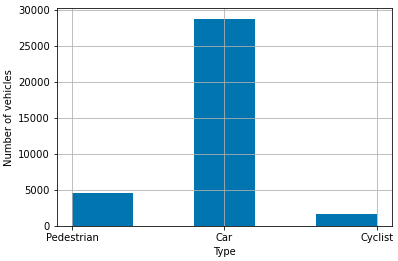
\includegraphics[width=0.4\textwidth]{Book/figures/6_approx_distancia/classes_kitti.png}
    \caption{Aparición de las clases en KITTI.}
    \label{fig:Aparición de las clases en KITTI.}
\end{figure}

Uno de los problemas más importantes a tener en cuenta dentro del dataset de KITTI es la pésima distribución de las clases con las que se trata. Como se observa en la Figura \ref{fig:Aparición de las clases en KITTI.}, en torno a un 80\% de objetos con los que se trabaja son coches por lo que es muy importante tener esto en cuenta, ya que no todas las clases tienen las misma características y puede influir negativamente en el ajuste de los modelos a diseñar. En cuanto a este hecho, la aplicación de técnicas de fine tuning presentadas en el Capítulo \ref{sec:Entrenamiento y evaluación de YOLOv5} para el entrenamiento del modelo de detección del objetos 2D consigue evitar parcialmente el sobreajuste que implica el uso de clases tan desbalanceadas.

\begin{figure}[H]
	\begin{minipage}{0.48\textwidth}
		\centering
		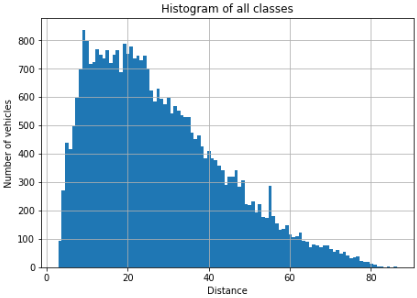
\includegraphics[width=0.97\linewidth]{Book/figures/6_approx_distancia/distance_kitti.png}
		\caption{Distribución de la distancia.}
		\label{fig:Distribución de la distancia.}
	\end{minipage}\hfill
	\begin{minipage}{0.45\textwidth}
		\centering
		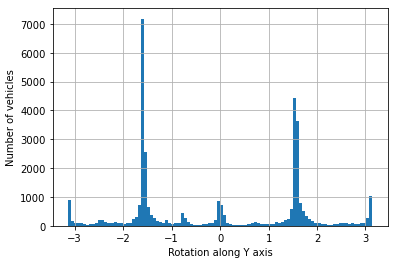
\includegraphics[width=1\linewidth]{Book/figures/6_approx_distancia/rotation_y_kitti.png}
		\caption{Distribución de la rotación.}
		\label{fig:Distribución de la rotación.}
	\end{minipage}
\end{figure}

De la misma que se ha  analizado los datos en relación al tipo de clase presente en el dataset, otras de las características más interesantes para su análisis son: la distribución de distancias a cada objeto del ground-truth y la rotación respecto del eje del propio vehículo del resto de objeto del entorno.

La Figura \ref{fig:Distribución de la distancia.} muestra la distribución de la distancia a los vehículos del ground-truth calculada como la distancia desde el origen del sistema de coordenadas de la cámara y el centro tridimensional de los objetos ($\sqrt{x^2+y^2+z^2}$). Esta distribución muestra como la mayoría de los objetos del ground-truth se encuentran entre los 10 y los 30 metros, además de encontrar objetos hasta una distancia de 80 metros, los cuales no se terminan evaluando debido a los diferentes niveles de dificultad que tiene KITTI (los cuales se presentarán más adelante) y que descartan el uso de estos objetos tan alejados. Estudiando la distancia por clases, se ha observado como los coches y ciclistas tienen su mayor presencia en torno a los 20 metros, mientras que los peatones tienen una mayor aparición a los 10 metros. En el caso de la detección 3D de los objetos se pretende conseguir unas detecciones relativamente buenas hasta los 50 metros, ya que a partir de esa distancia, se trabaja con muy pocos píxeles en la cámara y apenas puntos del \ac{LiDAR} lo que resulta en una tarea extremadamente compleja.

En cuanto a la rotación de los objetos del entorno respecto del vehículo propio, en la Figura \ref{fig:Distribución de la rotación.} se puede ver como los valores cercanos a $\pi/2$ y $-\pi/2$ son aquellos más prevalecientes en el dataset. Esto es debido a que este campo utiliza un sistema de rotación medido radianes donde el 0 apunta hacia la derecha del propio vehículo en \ac{BEV}. Por lo que se puede asumir directamente que lo más probable en cuanto a la orientación de todos los objetos de ground-truth es que se encuentren en la misma dirección pero puede ser el sentido puede ser el mismo o el opuesto, esto es muy probablemente debido a que la mayoría de los objetos del entorno a detectar se encuentran en los carriles, por lo que excepto en intersecciones esto va a ser correcto.

\begin{figure}[H]
    \centering
    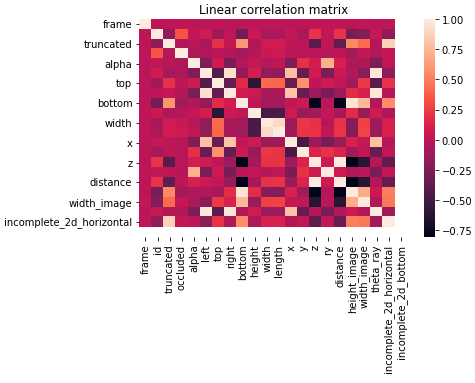
\includegraphics[width=0.6\textwidth]{Book/figures/6_approx_distancia/corr_matrix_kitti.png}
    \caption{Matriz de correlación de las características analizadas.}
    \label{fig:Matriz de correlación de las características analizadas.}
\end{figure}

Dentro de este mismo análisis se estudia de manera muy superficial las características del dataset que tienen una mayor relación con la distancia ya que es necesario obtener con que característica se puede obtener la distancia, tal y como se tratará se realizar en el siguiente capítulo. Para ello se construye una matriz de correlación mediante el uso del coeficiente de correlación de Pearson: $\rho_{X,Y} = \sigma_{X,Y}/(\sigma_X \sigma_Y)$. La Figura \ref{fig:Matriz de correlación de las características analizadas.} muestra dicha matriz de correlación en la que se observa como son: la recta horizontal inferior de la bounding box 2D, el eje Z del centro tridimensional, la altura de la bounding box 2D y la anchura de la bounding box 2D; aquellos parámetros que tienen un índice de correlación mayor con la distancia.

Habiendo obtenido las características más relevantes para la obtención de la distancia a los objetos, se visualiza en un gráfico de dispersión con la relación entre estos y la distancia, para obtener la característica a utilizar en la predicción de la distancia. La Figura \ref{fig:Gráficos de dispersión entre la distancia y las características con más correlación.} muestra todos los gráficos de dispersión, teniendo en el eje de ordenadas la distancia a los objetos y en el eje de abscisas las características estudiadas. En este gráfico se observa como a partir del eje Z del centro tridimensional se puede obtener directamente la distancia, de forma adicional, a partir de la recta horizontal inferior de la bounding box 2D y la altura de la bounding box 2D se puede obtener también la distancia pero con algo más de error, por último, con la la anchura de la bounding box 2D no se puede obtener la distancia de forma sencilla sin asumir un error muy grande.

\begin{figure}[H]
    \centering
    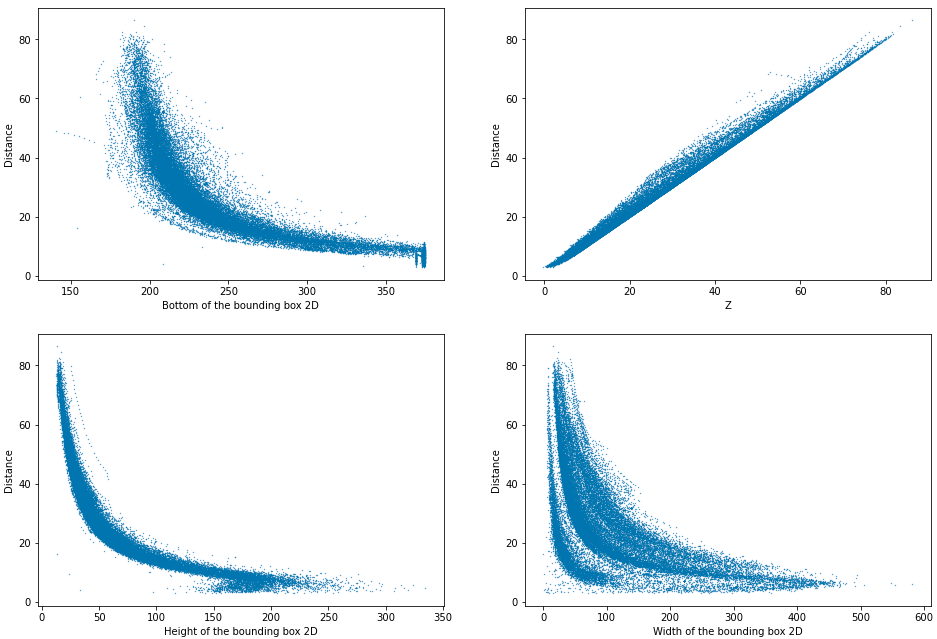
\includegraphics[width=0.9\textwidth]{Book/figures/6_approx_distancia/metrics_to_get_distance_kitti.png}
    \caption{Gráficos de dispersión entre la distancia y las características con más correlación.}
    \label{fig:Gráficos de dispersión entre la distancia y las características con más correlación.}
\end{figure}

Debido a que el eje Z del centro tridimensional de los objetos no se conoce de antemano, se decide utilizar para obtener la distancia a los objetos, la altura de la bounding box 2D. Esto es así, ya que de forma comparativa con la recta horizontal inferior de la bounding box 2D, se tiene una menor dispersión, además de estar asumiendo con este parámetro que el vehículo se encuentra siempre en una carretera sin pendientes, ya que el dataset de KITTI no contiene ninguna situación con esta característica.

\section{Modelo basado en la altura del objeto 2D}
\label{sec:Modelo basado en la altura del objeto 2D}

Habiendo elegido la característica que permite de mejor manera la obtención de la distancia, se trata de obtener una función que ajuste la distancia tras la obtención de la bounding box 2D de cada objeto. Este ajuste de la función no se realiza sobre la salida del modelo \ac{YOLO}v5, sino que parte del ground-truth de KITTI para su ajuste con los datos de entrenamiento, y se comprueba la efectividad de dicho ajuste sobre los datos de validación.

La métrica definida para la evaluación de todos los modelos de aproximación de la distancia es el \ac{MSE}, el cual se define por la siguiente función: $\textit{MSE} = \frac{1}{n} \sum_{i=1}^{n} (Y_i - \hat{Y}_i)^2$. Esta métrica es elegida ya que elimina los errores positivos y negativos, además de castigar de forma cuadrática los errores más grandes, lo cual permitirá discernir de mejor manera el modelo que más se ajusta.

En cuanto al modelo de ajuste, se decide optar por un sencillo modelo de regresión (no lineal) ya que permite su creación de forma sencilla además de permitir una ejecución de forma inmediata sin añadir carga de trabajo a todo el pipeline de detección 3D. Para realizar el ajuste de la función a utilizar que tenga de entrada la altura de la bounding box 2D y como salida la distancia al objeto, se utiliza la librería Scikit-learn. Mediante el uso de dicha librería en Python, se definen múltiples funciones polinómicas y logarítmicas para que mediante un ajuste por mínimos cuadrados se obtengan los valores que compongan las diferentes funciones.

En la Figura \ref{fig:Ajuste de diversas funciones para la obtención de la distancia.} se observan 6 de las funciones que se han probado para ajustar la obtención de la distancia. En esta imagen se observa como las funciones polinómicas no son capaces de ajustarse de forma correcta a las características de la curva definida por la relación entre las características analizadas. Por otra parte, las funciones funciones logarítmicas utilizadas son aquellas que mejor se ajustan, siendo la siguiente función aquella que mejor se ajusta: $y = a \log{x}^b + c; a = 668,12; b = -2; c = -17,39$.

\begin{figure}[H]
    \centering
    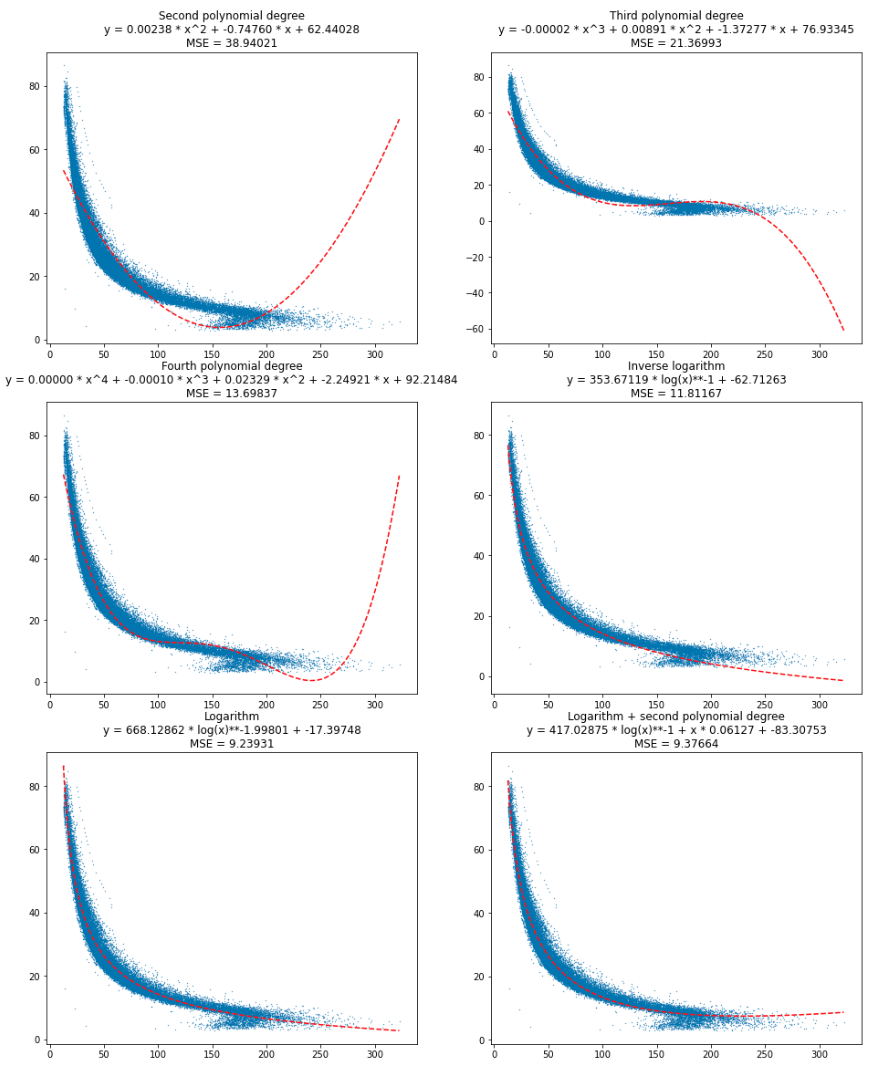
\includegraphics[width=0.7\textwidth]{Book/figures/6_approx_distancia/distance_regression_1_kitti1.png}
    \caption{Ajuste de diversas funciones para la obtención de la distancia.}
    \label{fig:Ajuste de diversas funciones para la obtención de la distancia.}
\end{figure}

Habiendo observado en el capítulo anterior que cada una de las clases de objetos utilizados tiene unas dimensiones diferentes, se plantea la creación de una función por cada una de las tres clases a detectar. Para ello se utilizará la función logarítmica previamente obtenida que se ajusta de mejor manera a los datos.

Tras la obtención de las parámetros de esta función logarítmica se obtienen las diferentes curvas que ajustan la relación entre la distancia y altura de la bounding box 2D para cada una de las clases. Esto se realiza de esta manera debido a que la altura media de cada una de las clases es diferente, por lo que el ajuste al realizarse de forma individual por cada clase de puede mejorar la precisión de las predicciones de la distancia a cada objeto. En la Figura \ref{fig:Ajuste de una función logarítmica por cada clase.} se observa como en las clases peatón y ciclista la métrica de \ac{MSE} se reduce, mientras que en la clase coche se aumenta. Esto es debido a que como se vio previamente, el 80\% de los objetos de los objetos son coches, por lo que se les puede encontrar en muchas más situaciones complejas.

\begin{figure}[H]
    \centering
    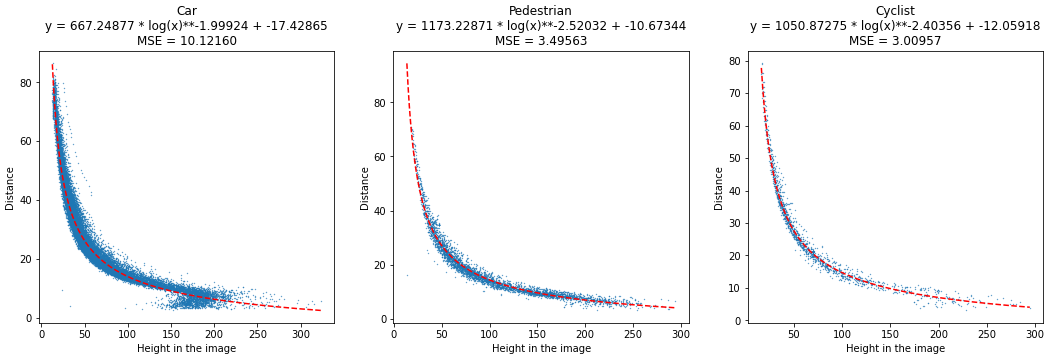
\includegraphics[width=1\textwidth]{Book/figures/6_approx_distancia/regression_classes_kitti1.png}
    \caption{Ajuste de una función logarítmica por cada clase.}
    \label{fig:Ajuste de una función logarítmica por cada clase.}
\end{figure}

Analizando el resto de características con las que se puede trabajar para obtener una aproximación de la distancia más precisa, se encuentra que la completitud horizontal de las bounding boxes 2D de los objetos, definida como aquellas bounding boxes que se encuentran en el límite izquierdo o derecho de la imagen, pueden aportar información al modelo, ya que aquellas bounding boxes que cumplen esta propiedad, no se conoce de forma correcta la altura de su bounding box 2D al no encontrarse el objeto al completo dentro del \ac{FoV} de la cámara. Se ha observado de forma adicional, como el análisis únicamente de la componente horizontal de la bounding box 2D aporta más información que el uso de la componente vertical o la combinación de ambas.

En la Figura \ref{fig:Resaltado de las bounding box 2D no completas horizontalmente.} se puede ver de forma resaltada en naranja aquellos objetos que cumplen con el filtro de bounding boxes 2D incompletas horizontalmente. En dichos puntos naranjas se observa una distribución diferente a la encontrada de forma general en el resto del dataset, por lo que se decide incorporar este parámetro al modelo a utilizar. 

\begin{figure}[H]
    \centering
    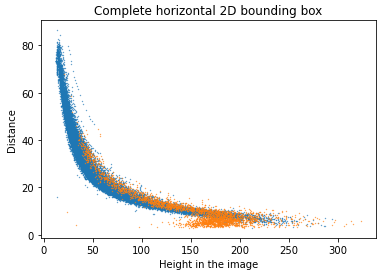
\includegraphics[width=0.5\textwidth]{Book/figures/6_approx_distancia/bb_complete_kitti1.png}
    \caption{Resaltado de las bounding box 2D no completas horizontalmente.}
    \label{fig:Resaltado de las bounding box 2D no completas horizontalmente.}
\end{figure}

Habiendo definido el uso de una nueva característica es necesario definir con que técnica tratarla, en este caso, al observarse en la figura anterior una nueva curva con los datos filtrados según la nueva característica a utilizar se decide ajustar de forma separada dos curvas logarítmicas como se ha hecho previamente. Durante el análisis de esta característica se ha observado que en las clases 'peatón' y 'ciclista' hay muy pocos casos en los que las bounding boxes 2D no se encuentren completas, debido a esto, para evitar un caso de sobreajuste se decide utilizar la clase 'coche' como la única por la que filtrar y ajustar una función en relación a la completitud de la bounding box 2D.

En la Figura \ref{fig:Ajuste de la distancia a los coches en función de la completitud de la bounding box 2D.} se muestra el ajuste de las dos curvas en función de la nueva característica a introducir en el modelo sobre la clase 'coche', de esta manera se consigue que las vehículos que cumplen esta característica tengan una distancia aproximada más precisa.

\begin{figure}[H]
	\begin{minipage}{0.45\textwidth}
		\centering
		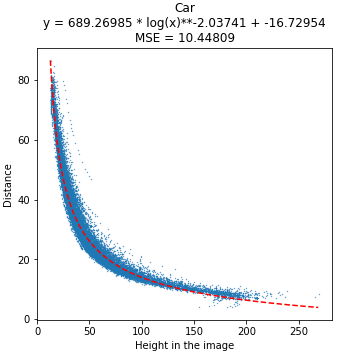
\includegraphics[width=0.87\linewidth]{Book/figures/6_approx_distancia/car_bb_complete_kitti1.png}
	\end{minipage}\hfill
	\begin{minipage}{0.45\textwidth}
		\centering
		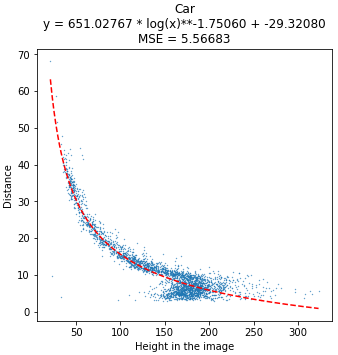
\includegraphics[width=0.9\linewidth]{Book/figures/6_approx_distancia/car_bb_incomplete_kitti1.png}
	\end{minipage}
	\caption{Ajuste de la distancia a los coches en función de la completitud de la bounding box 2D.}
	\label{fig:Ajuste de la distancia a los coches en función de la completitud de la bounding box 2D.}
\end{figure}

Como forma de estudiar los resultados obtenidos del sistema de aproximación de la distancia, se decide utilizar un método de evaluación común entre todos los modelos que sean diseñados, para ello se va a basar en el método de evaluación de KITTI y la métrica definida hasta ahora como es el \ac{MSE}.

Dentro de la evaluación de KITTI se define el concepto de dificultad entre los diferentes objetos a detectar, para los cuales se usa la altura de los objetos sobre la imagen, la oclusión (valor en función de la visibilidad del objeto que puede variar de 0 a 3) y el porcentaje de truncamiento de los objetos sobre el \ac{FoV} de la cámara. las diferentes dificultades con las que se trabaja son:
\begin{itemize}
    \item 'Fácil': son aquellos objetos con una altura en la imagen mayor de 40 píxeles, un valor de oclusión de 0 y un truncamiento máximo del 15\%.
    \item 'Moderado': son aquellos objetos con una altura en la imagen mayor de 25 píxeles, un valor de oclusión máximo de 1 y un truncamiento máximo del 30\%.
    \item Difícil: son aquellos objetos con una altura en la imagen mayor de 25 píxeles, un valor de oclusión máximo de 2 y un truncamiento máximo del 30\%.
\end{itemize}
El resto de los objetos que no se incluyen en ninguna de las diferentes categorías no se estudian, aunque más adelante se verá un caso en el que aquellos objetos sin dificultad han sido de relevancia.

Tras la definición del método de evaluación que se compone de las dificultades, la métrica (\ac{MSE}) y el estudio a nivel de clase, se calculan las métricas obtenidas en este primer método de aproximación de la distancia basado en la altura de las bounding boxes 2D.

\begin{table}[H]
\centering
\begin{tabular}{|c|c|c|c|}
\hline
\textbf{Benchmark (MSE)} & \textbf{Fácil} & \textbf{Moderado} & \textbf{Difícil} \\ \hline \hline
Coche (distancia)        & 8,724          & 9,115             & 9,127            \\ \hline
Peatón (distancia)       & 4,643          & 5,902             & 5,645            \\ \hline
Ciclista (distancia)     & 3,822          & 4,444             & 4,469            \\ \hline
\end{tabular}
\caption{Evaluación sobre KITTI del modelo de aproximación de distancia basado en regresión.}
\label{tab:Evaluación sobre KITTI del modelo de aproximación de distancia basado en regresión.}
\end{table}

La Tabla \ref{tab:Evaluación sobre KITTI del modelo de aproximación de distancia basado en regresión.} muestra unos resultados bastante buenos de este modelo de aproximación de distancia, el cual solo requiere de una imagen de las bounding boxes 2D que pueden ser obtenidas por un modelo como YOLOv5. Tras este primer modelo se estudiaran otros que traten de mejorar estos primeros resultados que son claramente bastante buenos pero mejorables.

\section{Modelo basado en la proyección de la nube de puntos}
\label{sec:Modelo basado en la proyección de la nube de puntos}

Habiendo obtenido un modelo de aproximación de la distancia basado únicamente en la cámara del vehículo, se ha decido utilizar también en un modelo diferente la nube de puntos proporcionada por el \ac{LiDAR}. Mientras que la cámara no tiene ningún método directo con el que calcular la distancia a los objetos, con el \ac{LiDAR} se puede calcular la distancia a cualquier punto de la nube de puntos obtenida por dicho sensor de forma precisa.

Partiendo del uso de bounding boxes 2D que pueden ser obtenidas por el modelo YOLOv5 presentado en la Sección \ref{sec:Entrenamiento y evaluación de YOLOv5}, se decide trabajar de forma conjunta con dichas detecciones 2D junto con el \ac{LiDAR} para analizar los puntos que se encuentran dentro de las bounding boxes. Mientras que esto parece una tarea sencilla es necesario estudiar las transformaciones de mundo a cámara de una lente como se observa en la Figura \ref{fig:Transformaciones mundo a cámara.} para poder pasar del sistema de coordenadas del LiDAR a la cámara.

\begin{figure}[H]
    \centering
    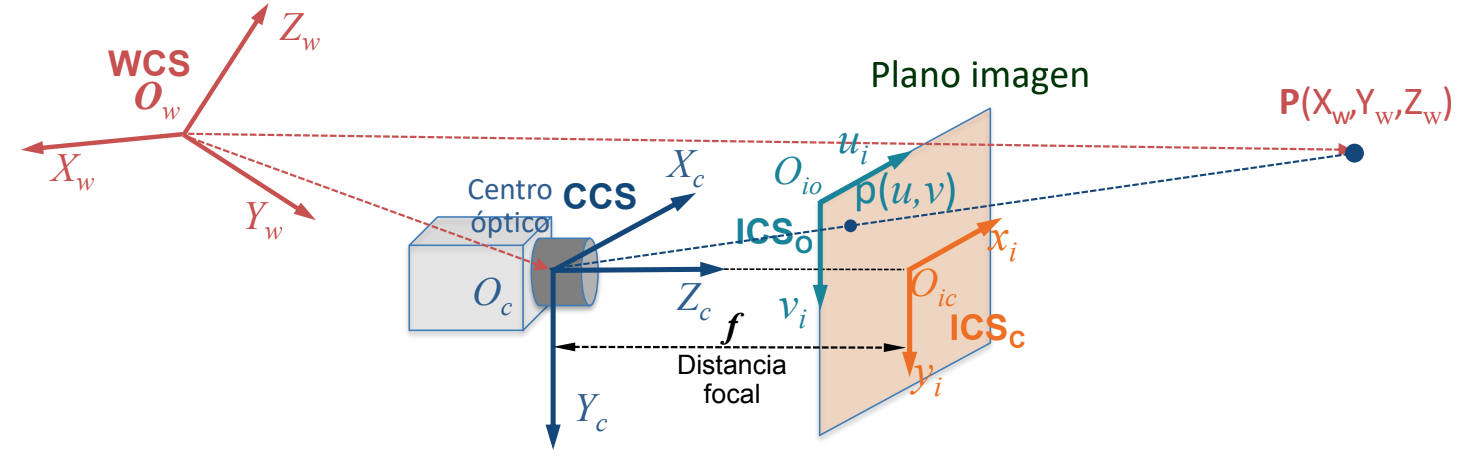
\includegraphics[width=0.7\textwidth]{Book/figures/6_approx_distancia/funcionamiento_camara.png}
    \caption{Transformaciones mundo a cámara.}
    \label{fig:Transformaciones mundo a cámara.}
\end{figure}

Tras el estudio de las transformaciones necesarias para obtener la nube de puntos sobre las imágenes obtenidas por la cámara se estudiaran los puntos para tratar de obtener un modelo que mejore al modelo anterior basado únicamente en la cámara. Para ello se plantea utilizar la mediana de la distancia de los puntos dentro de cada objeto y posteriormente se aplicará un pequeño modelo que obtenga la distancia al centro de cada objeto.

\subsection{Sistema de proyección de la nube de puntos a la cámara}
\label{sec:Sistema de proyección de la nube de puntos a la cámara}

Las nubes de puntos dadas en el dataset de KITTI siguen un formato típico en el cual a partir de un archivo binario se guarda la información de cada punto definida por los parámetros: 'x', 'y', 'z' y 'intensidad'; los cuales tienen un formato de números decimales de 32 bits. Dentro de las transformaciones geométricas a realizar solo es necesario utilizar las coordenadas tridimensionales de cada punto para realizar la traslación, rotación y cambio en el sistema de coordenadas de la nube de puntos. Para la comprensión de las operaciones realizadas en esta transformación es necesario comprender primero el funcionamiento de las proyecciones mundo a cámara las cuales son utilizadas en dicha proyección.

Como primer paso dentro de este proceso de la proyección de la nube de puntos a la cámara, es necesario el sistema de coordenadas a utilizar. En este caso se ha definido un sistema de coordenadas homogéneas para simplificar ciertos pasos más adelante, por lo que es necesario transformar el sistema de coordenadas cartesiano a este sistema de la manera definida por las siguientes fórmulas.

\begin{center}
$(x, y, z) \rightarrow (x', y', z', w)$\\[10pt]
$(x, y, z) = (x'/w, y'/w, z'/w)$
\end{center}

Tras la transformación al sistema de coordenadas homogéneo, se trata de cambiar el sistema de coordenadas actual al dado por la cámara con la que se trabaja, para ello es necesario realizar una traslación al sistema de coordenadas de la cámara y tras esto una rotación de los ejes para que concuerden con el sistema de coordenadas de la cámara. Al trabajar con las coordenadas homogéneas, la traslación del eje de coordenadas no es más que una multiplicación de matrices como se puede observa en la siguiente fórmula.

\begin{center}
$
\begin{bmatrix} wX_c \\ wY_c \\ wZ_c \\ w \end{bmatrix}
=
\begin{bmatrix}
1 & 0 & 0 & T_X \\
0 & 1 & 0 & T_Y \\
0 & 0 & 1 & T_Z \\
0 & 0 & 0 & 1 \\
\end{bmatrix}
\begin{bmatrix} X_w \\ Y_w \\ Z_w \\ 1 \end{bmatrix}
$
\end{center}

En cuanto a la rotación del sistema de coordenadas, es necesario entender que la rotación se realiza en los tres diferentes ejes, por lo que hay que utilizar una matriz de rotación por cada uno de los ejes, lo cual es una multiplicación de cuatro matrices.

\begin{center}
$R = R_X(\alpha) R_Y(\beta) R_Z(\gamma)$
\end{center}

\begin{center}
$
\begin{bmatrix} wX_c \\ wY_c \\ wZ_c \\ w \end{bmatrix}
=
\begin{bmatrix}
1 & 0 & 0 & 0 \\
0 & \cos \alpha & -\sin \alpha & 0 \\
0 & \sin \alpha & \cos \alpha & 0 \\
0 & 0 & 0 & 1 \\
\end{bmatrix}
\begin{bmatrix}
\cos \beta & 0 & \sin \beta & 0 \\
0 & 1 & 0 & 0 \\
- \sin \beta & 0 & \cos \beta & 0 \\
0 & 0 & 0 & 1 \\
\end{bmatrix}
\begin{bmatrix}
\cos \gamma & - \sin \gamma & 0 & 0 \\
\sin \gamma & \cos \gamma & 0 & 0 \\
0 & 0 & 1 & 0 \\
0 & 0 & 0 & 1 \\
\end{bmatrix}
\begin{bmatrix} X_w \\ Y_w \\ Z_w \\ 1 \end{bmatrix}
$
\end{center}

Otra opción es multiplicar desde un principio la matriz de traslación y las tres matrices de rotación que son fijas si no se mueve ninguno de los dos sistemas de coordenadas con los que se trabaja, y trabajar con una única matriz para reducir la complejidad de la fórmula además de reducir el numero de operación a realizar por un ordenador. Esta matriz es denominada la matriz de parámetros extrínsecos.

\begin{center}
$
\begin{bmatrix} wX_c \\ wY_c \\ wZ_c \\ w \end{bmatrix}
=
\begin{bmatrix}
\cos \gamma \cos \beta & - \sin \gamma \cos \beta & \sin \beta & T_X \\
\cos \gamma \sin \alpha \sin \beta + \sin \gamma \cos \alpha & \cos \gamma \cos \alpha - \sin \gamma \sin \alpha \sin \beta & - \sin \alpha \cos \beta & T_Y \\
\sin \gamma \sin \alpha - \cos \gamma \cos \alpha \sin \beta & \sin \gamma \cos \alpha \sin \beta + \cos \gamma \sin \alpha & \cos \alpha \cos \beta & T_Z \\
0 & 0 & 0 & 1 \\
\end{bmatrix}
\begin{bmatrix} X_w \\ Y_w \\ Z_w \\ 1 \end{bmatrix}
$
$
M_{ext}
=
\begin{bmatrix}
r_{11} & r_{12} & r_{13} & t_X \\
r_{21} & r_{22} & r_{23} & t_Y \\
r_{31} & r_{32} & r_{33} & t_Z \\
\end{bmatrix}
$
\end{center}

Tras este cambio del sistema de coordenadas al mismo con el que trabaja la cámara, es necesario pasar a nivel de píxel para comprender como cada punto del entorno tridimensional pasa a encontrarse dentro de las imágenes producidas por una cámara. Dentro de este proceso, es necesario comprender los parámetros intrínsecos que afectan en el paso del mundo real tridimensional al mundo bidimensional de las imágenes.

El primer parámetro a tener en cuenta es la distancia focal ($f$), la cual es la distancia entre el centro óptico de la lente y el foco de la cámara. Este parámetro es utilizado para pasar al sistema de coordenadas bidimensionales de la cámara pero en el sistema métrico.

\begin{center}
$
\begin{bmatrix} wx \\ wy \\ w \end{bmatrix}
=
\begin{bmatrix}
f & 0 & 0 & 0 \\
0 & f & 0 & 0 \\
0 & 0 & 1 & 0 \\
\end{bmatrix}
\begin{bmatrix} X_c \\ Y_c \\ Z_c \\ 1 \end{bmatrix}
$
\end{center}

Para obtener los puntos proyectados en los píxeles de las imágenes, se pasa al sistema de coordenadas pixélicas, definido por el tamaño en píxeles ($dx$, $dy$) y el desplazamiento al origen de las imágenes ($u_0$, $v_0$).

\begin{center}
$
\begin{bmatrix} wu \\ wv \\ w \end{bmatrix}
=
\begin{bmatrix}
1/dx & 0 & u_0 \\
0 & 1/dy & v_0 \\
0 & 0 & 1 \\
\end{bmatrix}
\begin{bmatrix} wx \\ wy \\ w \end{bmatrix}
$
\end{center}

De la misma manera que se construye la matriz de parámetros extrínsecos, se multiplican las dos últimas matrices relacionadas con los parámetros internos de la cámara, para construir una matriz de parámetros intrínsecos y simplificar el tratamiento de una cámara dada, ya que estos parámetros son fijos a una cámara concreta y no se modifican.

\begin{center}
$
M_{int}
=
\begin{bmatrix}
1/dx & 0 & u_0 \\
0 & 1/dy & v_0 \\
0 & 0 & 1 \\
\end{bmatrix}
\begin{bmatrix}
f & 0 & 0 \\
0 & f & 0 \\
0 & 0 & 1 \\
\end{bmatrix}
=
\begin{bmatrix}
f/dx & 0 & u_0 \\
0 & f/dy & v_0 \\
0 & 0 & 1 \\
\end{bmatrix}
$
\end{center}

De forma sencilla, se puede obtener la transformación de puntos tridimensionales del entorno a la cámara a partir de las matrices de parámetros extrínsecos e intrínsecos con unas simples multiplicaciones.

\begin{center}
$
\begin{bmatrix} wu \\ wv \\ w \end{bmatrix}
=
M_{int} M_{ext}
\begin{bmatrix} X_w \\ Y_w \\ Z_w \\ 1 \end{bmatrix}
$
\end{center}

Hasta ahora se ha explicado de forma teórica como funcionan las transformaciones necesarias para trabajar con cámara y comprender su tratamiento, pero en este apartado se explicará su uso práctico a partir de las matrices de calibración dadas en el dataset de KITTI y que han tenido que ser utilizadas para realizar todas las transformaciones geométricas necesarias en este apartado para la proyección de la nube de puntos además de su uso en la creación de 'troncos geométricos' como se verá en el Capítulo \ref{cha:Obtención de la región de interés}.

En este caso de uso concreto que se quiere obtener, es necesario trabajar con tres matrices diferentes con las que se logrará pasar del sistema de coordenadas de las nubes de puntos del \ac{LiDAR} a los píxeles de las imágenes dadas por el dataset de KITTI. Estas tres matrices son (según los nombres de dados por KITTI) las siguientes:

\begin{itemize}
    \item $P2$: Esta matriz se compone de la matriz intrínseca de la cámara 2, la cual es la cámara de la cual se van a utilizar las imágenes al ser aquella según se dan las detección 2D además de estar en color y no en escala de grises, además de la traslación respecto de la cámara 0 del vehículo utilizado para la creación de dataset.
    \item $R0\_rect$: Las lentes de la una cámara es muy difícil que sean perfectas, por lo que se suele aplicar una matriz de rectificación que tiene como función eliminar las imperfecciones en las imágenes como pueden ser las distorsiones de barril y de cojín. Esta matriz trata de solucionar estos problemas de las imágenes obtenidas por el sensor de la misma manera que se realiza con cual otro tipo de cámara (a menos que se trabaja con una lente con un error mínimo).
    \begin{center}
    $
    \textit{R0\_rect} = R_{Xr}(\alpha_r) R_{Yr}(\beta_r) R_{Zr}(\gamma_r) 
    \begin{bmatrix} 1&0&0&T_{Xr} \\ 0&1&0&T_{Yr} \\ 0&0&1&T_{Zr} \\ 0&0&0&1 \end{bmatrix}
    $
    \end{center}
    \item $Tr\_velo\_to\_cam$: Esta matriz se compone de la matriz de traslación del sistema de coordenadas del \ac{LiDAR} al sistema de coordenadas de la cámara 0 y de su correspondiente matriz de rotación.
    \begin{center}
    $
    \textit{Tr\_velo\_to\_cam} = R_{X\textit{v2c}}(\alpha_\textit{v2c}) R_{Yr}(\beta_\textit{v2c}) R_{Z\textit{v2c}}(\gamma_\textit{v2c}) 
    \begin{bmatrix} 1&0&0&T_{X\textit{v2c}} \\ 0&1&0&T_{Y\textit{v2c}} \\ 0&0&1&T_{Z\textit{v2c}} \\ 0&0&0&1 \end{bmatrix}
    $
    \end{center}
\end{itemize}

La conversión de la nube de puntos a las imágenes del dataset es muy sencilla si se conoce el funcionamiento de todas estas matriz, ya que simplemente es necesario multiplicar la nube de puntos completa por otras tres matrices diferentes como son: $P2$, $R0\_rect$ y $Tr\_velo\_to\_cam$.

\begin{center}
$
\textit{cam} = \textit{P2} * \textit{R0\_rect} * \textit{Tr\_velo\_to\_cam} * \textit{pcl}
$
\end{center}

\subsection{Aproximación de la distancia a partir de la nube de puntos}
\label{sec:Aproximación de la distancia a partir de la nube de puntos}

Partiendo del hecho que se conoce la manera de proyectar las nubes de puntos sobre las imágenes dadas, se abre una oportunidad para estudiar la distancia a los objetos a partir de dicha nube de puntos y las detecciones 2D que se pueden obtener de los objetos del entorno. La Figura \ref{fig:Proyección de la nube de puntos sobre la cámara.} muestra la manera en la que se proyecta la nube de puntos sobre la imagen que se da de entrada visualizando con colores la distancia del objeto con el colisiona cada láser del \ac{LiDAR} representado por un punto en la imagen.

\begin{figure}[H]
    \centering
    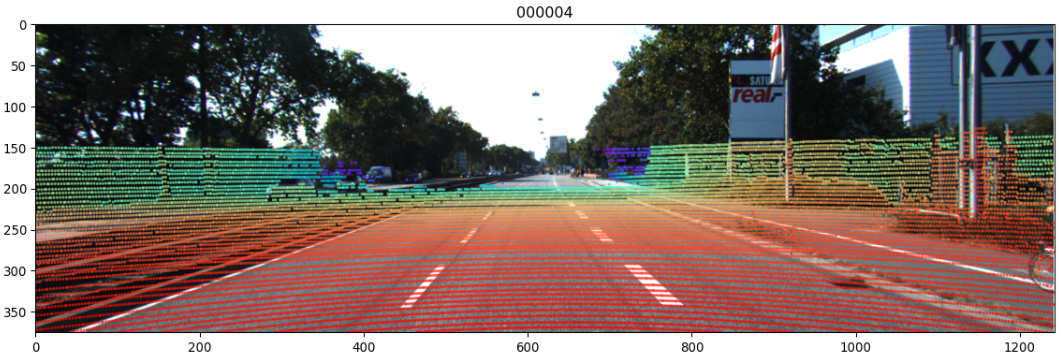
\includegraphics[width=0.8\textwidth]{Book/figures/6_approx_distancia/pcl_projection_kitti2.png}
    \caption{Proyección de la nube de puntos sobre la cámara.}
    \label{fig:Proyección de la nube de puntos sobre la cámara.}
\end{figure}

Mientras que el proceso de segmentación semántica puede ser muy útil y preciso para aproximar la distancia a los objetos del entorno, ya que permite utilizar solo los puntos que se encuentran en los vehículos y no aquellos puntos que no incidan en el objeto de interés, pero se deciden utilizar detecciones 2D ya que con modelos con esta tarea se pueden obtener de manera más rápida dichas detecciones además de diferenciar objetos diferentes si se encuentran muy cerca (cosa que no se puede con un modelo de segmentación semántica). En este análisis por tanto se usará el ground-truth 2D de las imágenes para la realización de las aproximaciones de la distancia a los objetos del entorno.

...

\begin{figure}[H]
    \centering
    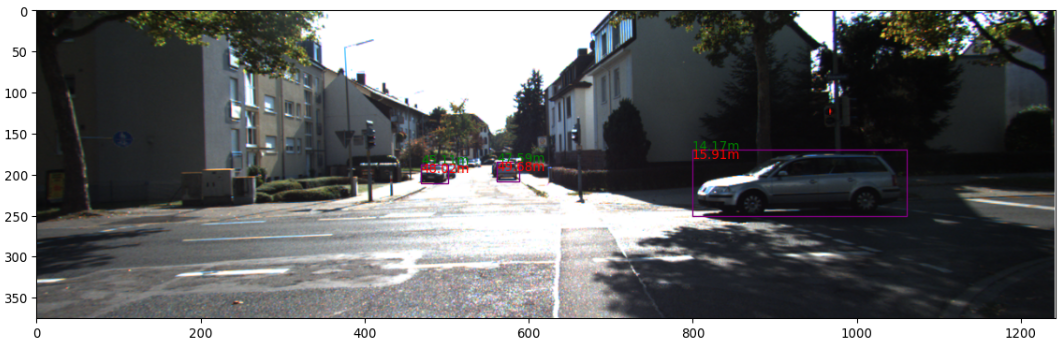
\includegraphics[width=0.8\textwidth]{Book/figures/6_approx_distancia/pcl_projection_distance_kitti2.png}
    \caption{Aproximación de la distancia mediante la nube de puntos.}
    \label{fig:Aproximación de la distancia mediante la nube de puntos.}
\end{figure}

\begin{table}[H]
\centering
\begin{tabular}{|c|c|c|c|c|}
\hline
\textbf{Benchmark (MSE)} & \textbf{Fácil} & \textbf{Moderado} & \textbf{Difícil} & \textbf{Todo}\\ \hline \hline
Coche (distancia)        & 4,084          & 15,759             & 29,198   &42,346         \\ \hline
Peatón (distancia)       & 3,355          & 6,223             & 13,516    &13,500         \\ \hline
Ciclista (distancia)     & 7,134          & 11,968             & 12,902   &12,857        \\ \hline
\end{tabular}
\caption{Evaluación del modelo de aproximación de distancia basado en nube de puntos.}
\label{fig:Evaluación sobre KITTI del primer modelo de aproximación de distancia basado en nube de puntos.}
\end{table}

\begin{figure}[H]
    \centering
    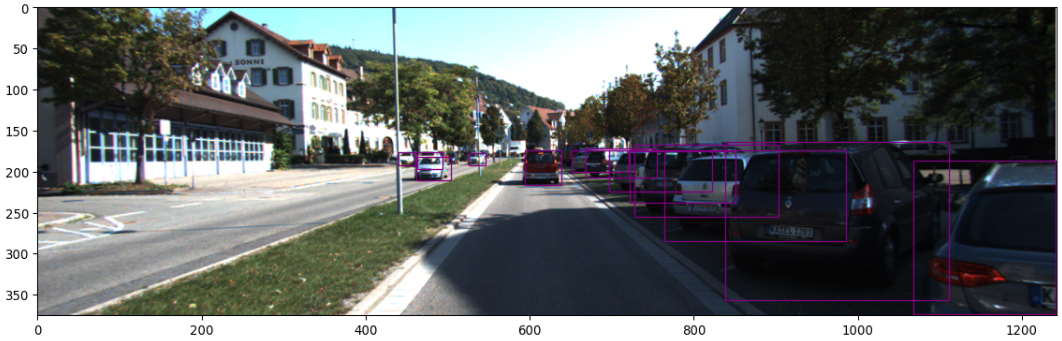
\includegraphics[width=0.8\textwidth]{Book/figures/6_approx_distancia/bb2d_kitti2.png}
    \caption{Caso de dificultad para obtener la distancia a partir de la nube de puntos.}
    \label{fig:Caso de dificultad para obtener la distancia a partir de la nube de puntos.}
\end{figure}

\begin{table}[H]
\centering
\begin{tabular}{|c|c|c|c|c|}
\hline
\textbf{Benchmark (MSE)} & \textbf{Fácil} & \textbf{Moderado} & \textbf{Difícil} & \textbf{Todo}\\ \hline \hline
Coche (distancia)        & 5,143          & 14,861             & 22,961       &29,971     \\ \hline
Peatón (distancia)       & 5,557          & 13,780             & 18,319       &18,032     \\ \hline
Ciclista (distancia)     & 7,107          & 19,733             & 30,106       &25,937  \\ \hline
\end{tabular}
\caption{Evaluación del modelo de aproximación de distancia sin intersecciones en las bounding boxes.}
\label{fig:Evaluación sobre KITTI del primer modelo de aproximación de distancia basado en nube de puntos.}
\end{table}

\subsection{Modelo de rectificación de la distancia}
\label{sec:Modelo de rectificación de la distancia}

\begin{figure}[H]
	\begin{minipage}{0.32\textwidth}
		\centering
		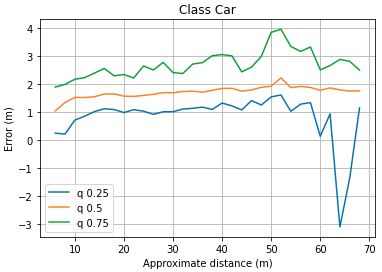
\includegraphics[width=1\linewidth]{Book/figures/6_approx_distancia/error_projection_car_kitti3.png}
	\end{minipage}\hfill
	\begin{minipage}{0.32\textwidth}
		\centering
		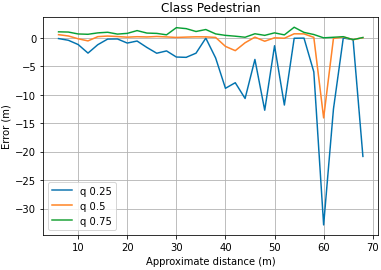
\includegraphics[width=1\linewidth]{Book/figures/6_approx_distancia/error_projection_pedestrian_kitti3.png}
	\end{minipage}\hfill
	\begin{minipage}{0.32\textwidth}
		\centering
		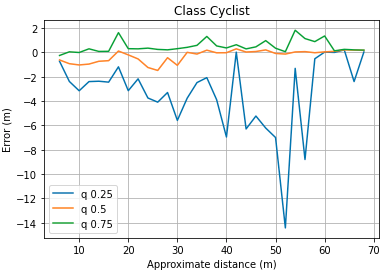
\includegraphics[width=1\linewidth]{Book/figures/6_approx_distancia/error_projection_cyclist_kitti3.png}
	\end{minipage}
	\caption{Error del modelo de de proyección con LiDAR por clase.}
	\label{fig:Error del modelo de de proyección con LiDAR por clase.}
\end{figure}

\begin{figure}[H]
    \centering
    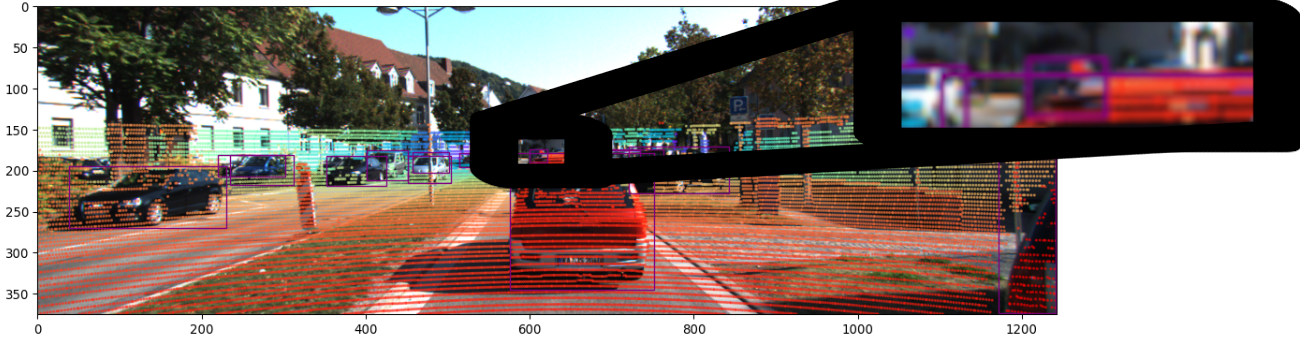
\includegraphics[width=0.8\textwidth]{Book/figures/6_approx_distancia/detail_lidar.png}
    \caption{Caso con gran error en la aproximación de la distancia.}
    \label{fig:Caso con gran error en la aproximación de la distancia.}
\end{figure}

\begin{figure}[H]
	\begin{minipage}{0.32\textwidth}
		\centering
		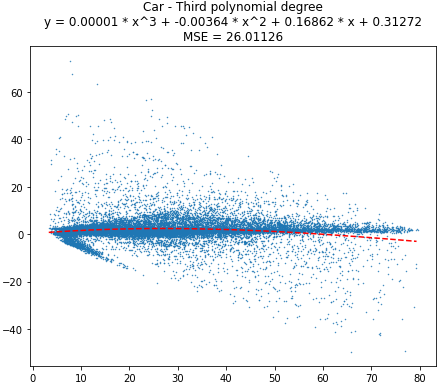
\includegraphics[width=1\linewidth]{Book/figures/6_approx_distancia/rectification_lidar_car.png}
	\end{minipage}\hfill
	\begin{minipage}{0.32\textwidth}
		\centering
		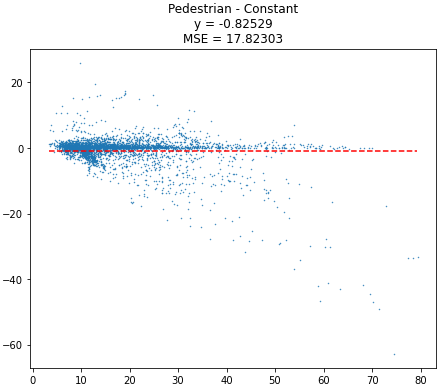
\includegraphics[width=1\linewidth]{Book/figures/6_approx_distancia/rectification_lidar_pedestrian.png}
	\end{minipage}\hfill
	\begin{minipage}{0.32\textwidth}
		\centering
		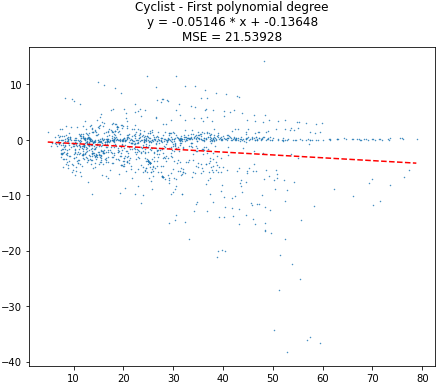
\includegraphics[width=1\linewidth]{Book/figures/6_approx_distancia/rectification_lidar_cyclist.png}
	\end{minipage}
	\caption{Modelo de rectificación de la distancia al centro de los objetos.}
	\label{fig:Modelo de rectificación de la distancia al centro de los objetos.}
\end{figure}

\begin{table}[H]
\centering
\begin{tabular}{|c|c|c|c|c|}
\hline
\textbf{Benchmark (MSE)} & \textbf{Fácil} & \textbf{Moderado} & \textbf{Difícil} & \textbf{Todo}\\ \hline \hline
Coche (distancia)        & 2,201          & 10,309             & 19,310       & 26,011     \\ \hline
Peatón (distancia)       & 5,557          & 13,780             & 18,319       & 18,032     \\ \hline
Ciclista (distancia)     & 4,911          & 15,778             & 24,367       & 21,540  \\ \hline
\end{tabular}
\caption{Evaluación del modelo de aproximación de distancia rectificado.}
\label{fig:Evaluación del modelo de aproximación de distancia rectificado.}
\end{table}

\begin{figure}[H]
	\begin{minipage}{0.32\textwidth}
		\centering
		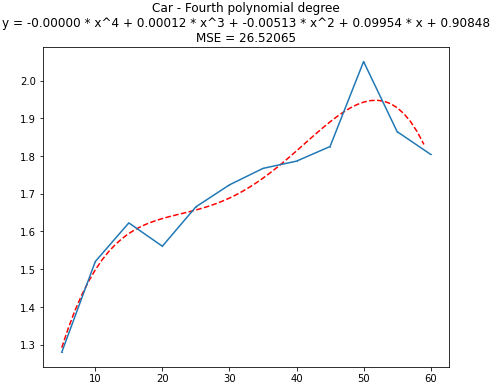
\includegraphics[width=1\linewidth]{Book/figures/6_approx_distancia/rectification2_lidar_car.png}
	\end{minipage}\hfill
	\begin{minipage}{0.32\textwidth}
		\centering
		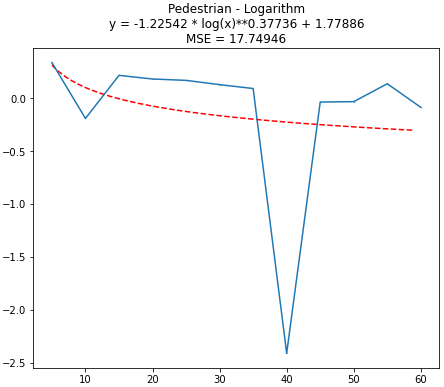
\includegraphics[width=1\linewidth]{Book/figures/6_approx_distancia/rectification2_lidar_pedestrian.png}
	\end{minipage}\hfill
	\begin{minipage}{0.32\textwidth}
		\centering
		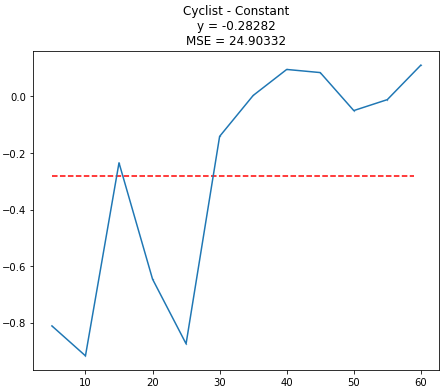
\includegraphics[width=1\linewidth]{Book/figures/6_approx_distancia/rectification2_lidar_cylist.png}
	\end{minipage}
	\caption{Modelo de rectificación de la distancia al centro de los objetos sin outliers.}
	\label{fig:Modelo de rectificación de la distancia al centro de los objetos sin outliers.}
\end{figure}

\begin{table}[H]
\centering
\begin{tabular}{|c|c|c|c|c|}
\hline
\textbf{Benchmark (MSE)} & \textbf{Fácil} & \textbf{Moderado} & \textbf{Difícil} & \textbf{Todo}\\ \hline \hline
Coche (distancia)        & 2,222          & 10,909             & 20,160       & 26,521     \\ \hline
Peatón (distancia)       & 5,467          & 13,691             & 18,198       & 17,912     \\ \hline
Ciclista (distancia)     & 6,404          & 18,799             & 29,000       & 24,903  \\ \hline
\end{tabular}
\caption{Evaluación del modelo de aproximación de distancia rectificado sin outliers.}
\label{fig:Evaluación del modelo de aproximación de distancia rectificado sin outliers.}
\end{table}

\section{Modelo de ensamble}
\label{sec:Modelo de ensamble}

\begin{figure}[H]
    \centering
    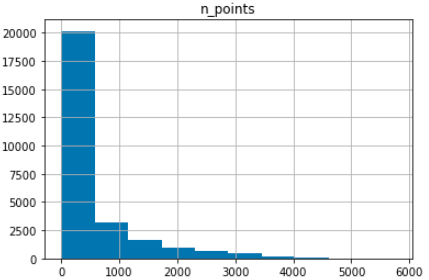
\includegraphics[width=0.4\textwidth]{Book/figures/6_approx_distancia/n_points_hist.png}
    \caption{Histograma con la cantidad de puntos sobre las bounding boxes 2D.}
    \label{fig:Histograma con la cantidad de puntos sobre las bounding boxes 2D.}
\end{figure}

\begin{figure}[H]
	\begin{minipage}{0.32\textwidth}
		\centering
		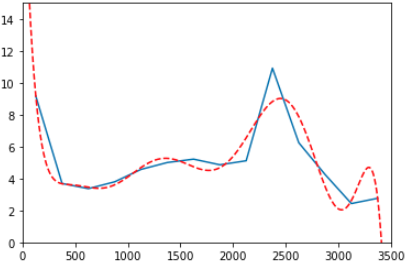
\includegraphics[width=1\linewidth]{Book/figures/6_approx_distancia/ensemble_overfitting_0.png}
	\end{minipage}\hfill
	\begin{minipage}{0.32\textwidth}
		\centering
		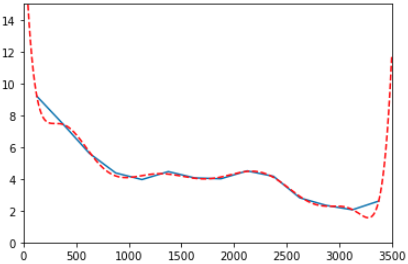
\includegraphics[width=1\linewidth]{Book/figures/6_approx_distancia/ensemble_overfitting_1.png}
	\end{minipage}\hfill
	\begin{minipage}{0.32\textwidth}
		\centering
		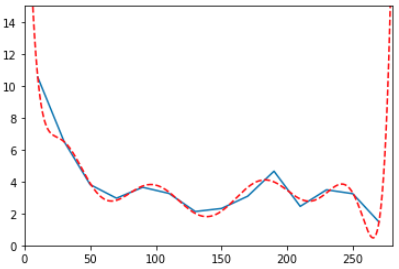
\includegraphics[width=1\linewidth]{Book/figures/6_approx_distancia/ensemble_overfitting_2.png}
	\end{minipage}
	\caption{Ajuste de las funciones de error de los modelos.}
	\label{fig:Ajuste de las funciones de error de los modelos.}
\end{figure}

\begin{figure}[H]
	\begin{minipage}{0.32\textwidth}
		\centering
		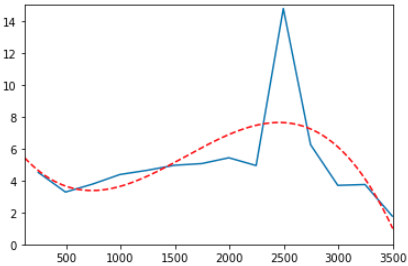
\includegraphics[width=1\linewidth]{Book/figures/6_approx_distancia/ensemble_not_overfitting_0.png}
	\end{minipage}\hfill
	\begin{minipage}{0.32\textwidth}
		\centering
		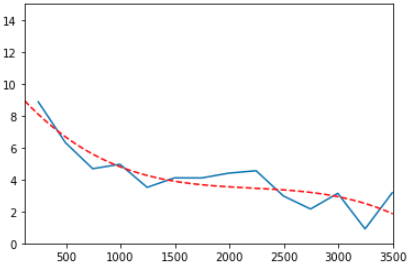
\includegraphics[width=1\linewidth]{Book/figures/6_approx_distancia/ensemble_not_overfitting_1.png}
	\end{minipage}\hfill
	\begin{minipage}{0.32\textwidth}
		\centering
		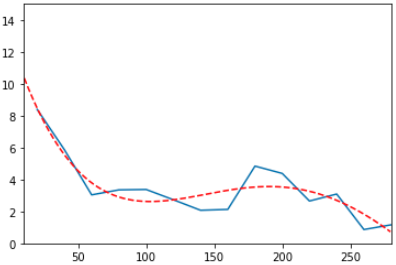
\includegraphics[width=1\linewidth]{Book/figures/6_approx_distancia/ensemble_not_overfitting_2.png}
	\end{minipage}
	\caption{Ajuste de las funciones de error de los modelos sin overfitting.}
	\label{fig:Ajuste de las funciones de error de los modelos sin overfitting.}
\end{figure}

\begin{table}[H]
\centering
\begin{tabular}{|c|c|c|c|}
\hline
\textbf{Benchmark (MSE)} & \textbf{Fácil} & \textbf{Moderado} & \textbf{Difícil}\\ \hline \hline
Coche (distancia)        & 2,137          & 6,499             & 8,618\\ \hline
Peatón (distancia)       & 1,916          & 2,802             & 3,430\\ \hline
Ciclista (distancia)     & 2,214          & 5,038             & 6,335\\ \hline
\end{tabular}
\caption{Evaluación del modelo ensemble utilizando los deciles de los errores.}
\label{fig:Evaluación del modelo ensemble utilizando los deciles de los errores.}
\end{table}

\begin{table}[H]
\centering
\begin{tabular}{|c|c|c|c|}
\hline
\textbf{Benchmark (MSE)} & \textbf{Fácil} & \textbf{Moderado} & \textbf{Difícil}\\ \hline \hline
Coche (distancia)        & 2,061          & 6,824             & 8,863\\ \hline
Peatón (distancia)       & 1,836          & 2,339             & 2,691\\ \hline
Ciclista (distancia)     & 2,007          & 4,26             & 4,834\\ \hline
\end{tabular}
\caption{Evaluación del modelo ensemble utilizando los deciles de los errores cuadráticos.}
\label{fig:Evaluación del modelo ensemble utilizando los deciles de los errores cuadráticos.}
\end{table}

\begin{table}[H]
\centering
\begin{tabular}{|c|c|c|c|}
\hline
\textbf{Benchmark (MSE)} & \textbf{Fácil} & \textbf{Moderado} & \textbf{Difícil}\\ \hline \hline
Coche (distancia)        & 3,011          & 6,608             & 6,972\\ \hline
Peatón (distancia)       & 1,786          & 2,327             & 2,757\\ \hline
Ciclista (distancia)     & 1,542          & 3,030             & 3,379\\ \hline
\end{tabular}
\caption{Evaluación del modelo ensemble utilizando los centiles de los errores.}
\label{fig:Evaluación del modelo ensemble utilizando los centiles de los errores.}
\end{table}

\begin{table}[H]
\centering
\begin{tabular}{|c|c|c|c|}
\hline
\textbf{Benchmark (MSE)} & \textbf{Fácil} & \textbf{Moderado} & \textbf{Difícil}\\ \hline \hline
Coche (distancia)        & 3,721          & 7,459             & 7,286\\ \hline
Peatón (distancia)       & 1,927          & 2,383             & 2,690\\ \hline
Ciclista (distancia)     & 1,540          & 2,611             & 2,631\\ \hline
\end{tabular}
\caption{Evaluación del modelo ensemble utilizando los centiles de los errores cuadráticos.}
\label{fig:Evaluación del modelo ensemble utilizando los centiles de los errores cuadráticos.}
\end{table}

\begin{table}[H]
\centering
\begin{tabular}{|ll|}
\hline
\multicolumn{2}{|c|}{\textbf{Errores}}       \\ \hline
\multicolumn{1}{|l|}{\textbf{1\%}}  & -4.809 \\ \hline
\multicolumn{1}{|l|}{\textbf{5\%}}  & -3.460 \\ \hline
\multicolumn{1}{|l|}{\textbf{50\%}} & -0.372 \\ \hline
\multicolumn{1}{|l|}{\textbf{95\%}} & 4.005  \\ \hline
\multicolumn{1}{|l|}{\textbf{99\%}} & 7.044  \\ \hline
\end{tabular}
\caption{Centiles del error del modelo final de la aproximación de la distancia.}
\label{fig:Centiles del modelo final de la aproximación de la distancia.}
\end{table}

\section{Análisis del error con YOLOv5}
\label{sec:Análisis del error con YOLOv5}

\begin{table}[H]
\centering
\begin{tabular}{|c|c|c|c|}
\hline
\textbf{Benchmark (MSE)} & \textbf{Fácil} & \textbf{Moderado} & \textbf{Difícil}\\ \hline \hline
Coche (distancia)        & 3.296          & 7.349             & 7.072\\ \hline
Peatón (distancia)       & 2.030          & 2.417             & 2.807\\ \hline
Ciclista (distancia)     & 2.207          & 3.787             & 3.803\\ \hline
\end{tabular}
\caption{Evaluación del modelo ensemble sobre las detecciones obtenidas del modelo YOLOv5m.}
\label{fig:Evaluación del modelo ensemble sobre las detecciones obtenidas del modelo YOLOv5m.}
\end{table}
\chapter{Obtención de la región de interés}
\label{cha:Obtención de la región de interés}

\begin{FraseCelebre}
  \begin{Frase}
    Texto.
  \end{Frase}
  \begin{Fuente}
    Autor texto
  \end{Fuente}
\end{FraseCelebre}

\section{Proyección de píxeles en la cámara a coordenadas 3D}
\label{sec:Proyección de píxeles en la cámara a coordenadas 3D}

\section{Obtención del tronco geométrico}
\label{sec:Obtención del tronco geométrico}

Rotación de eje frontal como en Frustum PointNets
\chapter{Sistema de detección 3D con LiDAR}
\label{cha:Sistema de detección 3D con LiDAR}

\begin{FraseCelebre}
  \begin{Frase}
    Texto.
  \end{Frase}
  \begin{Fuente}
    Autor texto
  \end{Fuente}
\end{FraseCelebre}

\section{Técnicas de detección 3D con LiDAR}
\label{sec:Técnicas de detección 3D con LiDAR}

\subsection{Voxelización}
\label{sec:Voxelización}

\subsection{Técnicas de Deep Learning aplicadas a detección 3D}
\label{sec:Técnicas de Deep Learning aplicadas a detección 3D}

\subsubsection{3D Convolutional Neural Networks}
\label{sec:3D Convolutional Neural Networks}

\subsubsection{Sparse Convolutions}
\label{sec:Sparse Convolutions}

\subsubsection{Single Shot Detectors}
\label{sec:Single Shot Detectors}

\subsubsection{Region Proposal Networks}
\label{sec:Region Proposal Networks}

\section{Modelos de detección 3D con LiDAR}
\label{sec:Modelos de detección 3D con LiDAR}

\subsection{PointNet}
\label{sec:PointNet}

\subsection{VoxelNet}
\label{sec:VoxelNet}

\subsection{SECOND}
\label{sec:SECOND}

\subsection{PointPillars}
\label{sec:PointPillars}

%Relación con MV3D (fase BEV)
%Selección basada en métricas de PointPainting

\section{Creación de un dataset de entrada para el modelo}
\label{sec:Creación de un dataset de entrada para el modelo}

\section{Entrenamiento y evaluación de Frustum PointPillars}
\label{sec:Entrenamiento y evaluación de Frustum PointPillars}

\chapter{Sistema completo de fusión sensorial}
\label{cha:Sistema completo de fusión sensorial}

\begin{FraseCelebre}
  \begin{Frase}
    Texto.
  \end{Frase}
  \begin{Fuente}
    Autor texto
  \end{Fuente}
\end{FraseCelebre}

\section{Resumen de todo el modelo de detección 3D}
\label{sec:Resumen de todo el modelo de detección 3D}

Pasos eliminados respecto de  Frustum PointNets

Tiempos: Comparación con PointPainting (para mostrar hasta donde se puede mejorar el tiempo de las transformaciones geométricas)

\section{Evaluación sobre KITTI}
\label{sec:Evaluación sobre KITTI}

\chapter{Conclusiones y trabajos futuros}
\label{cha:Conclusiones y trabajos futuros}

\begin{FraseCelebre}
  \begin{Frase}
    Texto.
  \end{Frase}
  \begin{Fuente}
    Autor texto
  \end{Fuente}
\end{FraseCelebre}

\section{Conclusiones}
\label{sec:Conclusiones}

\section{Trabajos futuros}
\label{sec:Trabajos futuros}

%%%%%%%%%%%%%%%%%%%%%%%%%%%%%%%%%%%%%%%%%%%%%%%%%%%%%%%%%%%%%%%%%%%%%%%%%%%%%%%%%%%%%%%%%%%%%%%%%%%%%%%%

%
% END Normal chapters. Edit/modify all within this section
%%%%%%%%%%%%%%%%%%%%%%%%%%%%%%%%%%%%%%%%%%%%%%%%%%%%%%%%%%%%%%%%%%%%%%%%%%%
%%%%%%%%%%%%%%%%%%%%%%%%%%%%%%%%%%%%%%%%%%%%%%%%%%%%%%%%%%%%%%%%%%%%%%%%%%%
%%%%%%%%%%%%%%%%%%%%%%%%%%%%%%%%%%%%%%%%%%%%%%%%%%%%%%%%%%%%%%%%%%%%%%%%%%%
%%%%%%%%%%%%%%%%%%%%%%%%%%%%%%%%%%%%%%%%%%%%%%%%%%%%%%%%%%%%%%%%%%%%%%%%%%%
%%%%%%%%%%%%%%%%%%%%%%%%%%%%%%%%%%%%%%%%%%%%%%%%%%%%%%%%%%%%%%%%%%%%%%%%%%%
%%%%%%%%%%%%%%%%%%%%%%%%%%%%%%%%%%%%%%%%%%%%%%%%%%%%%%%%%%%%%%%%%%%%%%%%%%%
%%%%%%%%%%%%%%%%%%%%%%%%%%%%%%%%%%%%%%%%%%%%%%%%%%%%%%%%%%%%%%%%%%%%%%%%%%%


%%%%%%%%%%%%%%%%%%%%%%%%%%%%%%%%%%%%%%%%%%%%%%%%%%%%%%%%%%%%%%%%%%%%%%%%%%%
% Bibliography
%%%%%%%%%%%%%%%%%%%%%%%%%%%%%%%%%%%%%%%%%%%%%%%%%%%%%%%%%%%%%%%%%%%%%%%%%%%
%%%%%%%%%%%%%%%%%%%%%%%%%%%%%%%%%%%%%%%%%%%%%%%%%%%%%%%%%%%%%%%%%%%%%%%%%%%
%
% Generic template for TFC/TFM/TFG/Tesis
%
% $Id: bibliography.tex,v 1.9 2015/06/05 00:10:32 macias Exp $
%
% By:
%  + Javier Macías-Guarasa. 
%    Departamento de Electrónica
%    Universidad de Alcalá
%  + Roberto Barra-Chicote. 
%    Departamento de Ingeniería Electrónica
%    Universidad Politécnica de Madrid   
% 
% Based on original sources by Roberto Barra, Manuel Ocaña, Jesús Nuevo,
% Pedro Revenga, Fernando Herranz and Noelia Hernández. Thanks a lot to
% all of them, and to the many anonymous contributors found (thanks to
% google) that provided help in setting all this up.
%
% See also the additionalContributors.txt file to check the name of
% additional contributors to this work.
%
% If you think you can add pieces of relevant/useful examples,
% improvements, please contact us at (macias@depeca.uah.es)
%
% You can freely use this template and please contribute with
% comments or suggestions!!!
%
%%%%%%%%%%%%%%%%%%%%%%%%%%%%%%%%%%%%%%%%%%%%%%%%%%%%%%%%%%%%%%%%%%%%%%%%%%%

%\bibliographystyle{plainnat}
%\bibliographystyle{dinat}
%\bibliographystyle{unsrt}
\bibliographystyle{IEEEtran}

% The following is overly complicated because I was not able to do so in
% another way. The problem is the bibliography command being "called"
% from both the root and anteproyecto directories...
%
% Here define as many bibfiles as needed
\newcommand{\mybibfileOne}{biblio/biblio.bib}
%\newcommand{\mybibfileTwo}{biblio/biblio2.bib}
%...
%\newcommand{\mybibfileN}{biblio/biblioN}

% This is for a single bib file
\newcommand{\mybibfiles}{\myreferencespath\mybibfileOne}
% but do this for multiple files
%\newcommand{\mybibfiles}{\myreferencespath\mybibfile1,\myreferencespath\mybibfile2,...,\myreferencespath\mybibfileN}

% Do not touch this
%\inputencoding{latin1}
\bibliography{\mybibfiles}
%\inputencoding{utf8}

%%% Local Variables:
%%% TeX-master: "../book"
%%% coding: utf-8
%%% End:


               % EDIT this file if required


%%%%%%%%%%%%%%%%%%%%%%%%%%%%%%%%%%%%%%%%%%%%%%%%%%%%%%%%%%%%%%%%%%%%%%%%%%%
% BEGIN Appendices. Edit/modify all within this section
%
% I don't recommend it, but if you want to define "parts", use this...
% BEWARE: I didn't write the english dependent code
%\part*{Apéndices}
%\label{part:apendices}

%\appendix                                         % DO NOT TOUCH THIS LINE!

%%%%%%%%%%%%%%%%%%%%%%%%%%%%%%%%%%%%%%%%%%%%%%%%%%%%%%%%%%%%%%%%%%%%%%%%%%%%%%%%%%%%%%%%%%%%%%%%%%%%%%%%
\begin{appendices}
  %\chapter{Manual de usuario}
\label{cha:Manual de usuario}
  %\chapter{Pliego de Condiciones}
\label{cha:Pliego de Condiciones}
  %\chapter{Presupuesto}
\label{cha:Presupuesto}
\end{appendices}
%%%%%%%%%%%%%%%%%%%%%%%%%%%%%%%%%%%%%%%%%%%%%%%%%%%%%%%%%%%%%%%%%%%%%%%%%%%%%%%%%%%%%%%%%%%%%%%%%%%%%%%%
%
% END Appendices. Edit/modify all within this section
%%%%%%%%%%%%%%%%%%%%%%%%%%%%%%%%%%%%%%%%%%%%%%%%%%%%%%%%%%%%%%%%%%%%%%%%%%%

%%%%%%%%%%%%%%%%%%%%%%%%%%%%%%%%%%%%%%%%%%%%%%%%%%%%%%%%%%%%%%%%%%%%%%%%%%%
% Now start text and numbering for backmatter (just backpage in our
% case)
%%%%%%%%%%%%%%%%%%%%%%%%%%%%%%%%%%%%%%%%%%%%%%%%%%%%%%%%%%%%%%%%%%%%%%%%%%%
\backmatter                                       % DO NOT TOUCH THIS LINE!

%%%%%%%%%%%%%%%%%%%%%%%%%%%%%%%%%%%%%%%%%%%%%%%%%%%%%%%%%%%%%%%%%%%%%%%%%%%
% Just for TFGs at UAH right now, but kept here JIC anybody else wants
% to use it
%%%%%%%%%%%%%%%%%%%%%%%%%%%%%%%%%%%%%%%%%%%%%%%%%%%%%%%%%%%%%%%%%%%%%%%%%%%
\input{cover/backpage.tex}                    % EDIT this file if
                                              % required, or comment it out

\end{document}

